\Chapter{Adatfeldolgozás és gépi tanulás}
\label{Chap:dokumen}

\iffalse
Ebben a fejezetben kell a hallgatónak leírnia a saját eredményeit. Például ilyennek tekinthető a hallgató által elkészített program leírása, algoritmus leírása alkalmazási lehetőségek, eredmények. Lehet benne több alfejezet vagy al-alfejezet is. Ezek számozása és a tartalomjegyzékben  való megjelenítése rögzített. A fejezet címe megváltoztatható az eredmények szerint. Ez a fejezet és a \aref{Chap:tema} együtt összesen 25-60 oldal terjedelmű kell hogy legyen
\fi

Az Elméleti kifejtés során meghatározott célokat különböző gépi tanulási módszerekkel lehet megoldani amik eltérő eredménnyel, pontossággal fognak működni. A nehézségi osztályok meghatározására elsősorban a  \myaref{ssec:klaszterezes} pontban részletezett klaszterezési módszerek használhatóak

\Section{Adathalmaz előkészítés}
A fejlesztés legelső lépése a megfelelő adatstruktúrára kialakítása és az adathalmaz tisztítása, ezzel megkönnyítve a későbbi feldolgozást valamint növelve a gépi tanulási algoritmusok pontosságát.

A struktúrát meghatározza az adattárolásra használt csv fájl szerkezete, ahol minden sor egy-egy megtett útvonalat jelöl az oszlopnevekben meghatározott jellemzők alapján. Ennek a fájlnak a betöltésre a Pandas \cite{python-pandas} nevű Python csomag szolgál, az adatok futás közbeni tárolására a csomagnak a DataFrame nevű adatstruktúrája kerül felhasználásra. A DataFrame kényelmes, ember közeli adatkezelést tesz lehetővé, az adatok oszlopnév és index alapján is könnyen elérhetőek, szűrhetőek.


%\SubSection{Adatstruktúra kialakítása}
%Az adatgyűjtés elsődleges eszközeként a szakdolgozat keretein belül készített weboldal szolgált, amely minden információt egy JSON alapú adatbázisban tárolt le. Az adathalmaz előkészítésének a legelső lépése a JSON struktúráról való áttérés egy, a Python programozási nyelv által kezelt, könnyen használható adatstruktúrára. Erre a szakdolgozat során a Pandas \cite{python-pandas} nevű Python csomag által megvalósított DataFrame nevű struktúra fog szolgálni , amely segítségével az adatokat táblázathoz hasonló formában lehet tárolni. Egy DataFrame oszlopai egyedi, a fejlesztő által definiált oszlopnevekkel érhetőek el, soraira index használatával lehet hivatkozni. Az oszlopok egyenként különböző típusúak lehetnek és tartalmazhatnak NULL értékeket. A DataFrame egyik legnagyobb előnye az oszlopok nevesítése, amivel könnyen nyomon követhető hogy az aktuális értékek melyik jellemzőnek felelnek meg, mit reprezentálnak a valóságban



%A fenti parancs segítéségével nem csak átalakításra kerül az adatstruktúra hanem megtörténik egy kezdetleges jellemző (feature) kiválasztás is. Törlésre kerül a külső azonosító (\textit{external\_id}) valamint a térképhez tartozó összes jellemző (\textit{map\_id}, \textit{map\_resource}, \textit{map\_summary}).

\SubSection{Adattisztítás}
A megfelelő adatstruktúra kialakítása után a következő lépés az adatok megtisztítása. Ez a lépés azért szükséges mert a legfigyelmesebben gyűjtött adathalmaz is tartalmazhat rossz értékeket, illetve előfordulhat hogy több helyen hiányzik a valódi érték. Ezeknek a hibáknak a megtalálása és kijavítása több fázisból áll.

%\csvautotabular{adat/rawDataDescription.csv}
A megtaláláshoz első lépés az adatok áttekintése: NULL értékek vizsgálata, egyes jellemzők eloszlásának megtekintése, minimum, maximum és a kvantilisek összehasonlítása. Ehhez nyújt segítséget a \myref{tab:rawDataDescription} táblázat amely a numerikus oszlopokról készült általános jellemzést összegzi. A táblázat oszlopainak a jelentése:
\begin{table}[!h]
	\resizebox{\textwidth}{!}{%
		\begin{tabular}{l|l|l|l|l|l|l|l|l|}
			\cline{2-9}
			& \multicolumn{1}{c|}{\textbf{Count}} & \multicolumn{1}{c|}{\textbf{Mean}} & \multicolumn{1}{c|}{\textbf{STD}} & \multicolumn{1}{c|}{\textbf{Min}} & \multicolumn{1}{c|}{\textbf{0.25}} & \multicolumn{1}{c|}{\textbf{0.50}} & \multicolumn{1}{c|}{\textbf{0.75}} & \multicolumn{1}{c|}{\textbf{Max}} \\ \hline
			\multicolumn{1}{|l|}{
				\textbf{age\_group}}  & 10014  & 1.01   & 0.48   & 0.0   & 1.0   & 1.0   & 1.0   & 2.0   \\ \hline
			\multicolumn{1}{|l|}{
				\textbf{average\_speed}}  & 10014   & 24.25   & 653.31  & 0.0  & 4.96   & 5.73  & 6.47  & 36100.0  \\ \hline
			\multicolumn{1}{|l|}{
				\textbf{average\_watts}}  & 1848  & 163.0  & 49.51  & 0.0  & 139.10  & 161.85  & 180.85 & 482.6 \\ \hline
			\multicolumn{1}{|l|}{
				\textbf{distance}} & 10014  & 26153.09 & 29465.23 & 0.0   & 7444.83 & 13751.25 & 34587.2  & 436806.0  \\ \hline
			\multicolumn{1}{|l|}{
				\textbf{elapsed\_time}} & 10014 & 5845.88 & 19296.2  & 0.0  & 1648.00  & 3020.0  & 7343.0  & 1806211.0  \\ \hline
			\multicolumn{1}{|l|}{
				\textbf{elev\_high}} & 9845 & 282.1 & 272.66 & -71.2  & 162.2  & 229.4  & 296.4 & 12103.0  \\ \hline
			\multicolumn{1}{|l|}{
				\textbf{elev\_low}}  & 9844  & 131.99 & 68.68  & -500.0  & 103.1 & 130.0 & 148.3  & 1484.0 \\ \hline
			\multicolumn{1}{|l|}{
				\textbf{kilojoules}} & 1765 & 1295.76 & 756.06 & 0.0 & 728.7 & 1236.7 & 1745.4  & 5928.8   \\ \hline
			\multicolumn{1}{|l|}{
				\textbf{max\_speed}} & 10014  & 12.14 & 3.99  & 0.0  & 9.6 & 11.6  & 14.48  & 122.7        \\ \hline
			\multicolumn{1}{|l|}{
				\textbf{max\_watts}} & 546 & 630.95  & 244.34  & 115.0 & 502.0 & 603.0  & 708.0 & 2428.0   \\ \hline
			\multicolumn{1}{|l|}{
				\textbf{moving\_time}}  & 10014  & 4543.18  & 5016.52  & 0.0 & 1442.0  & 2451.0  & 6109.0  & 90983.0  \\ \hline
			\multicolumn{1}{|l|}{
				\textbf{\begin{tabular}[c]{@{}l@{}}total\_elevation\\ \_gain\end{tabular}}}  & 10014  & 278.7  & 428.88  & 0.0  & 27.5   & 85.2 & 361.8   & 4416.8   \\ \hline
			\multicolumn{1}{|l|}{
				\textbf{\begin{tabular}[c]{@{}l@{}}weighted\_average\\ \_watts\end{tabular}}} & 546  & 188.86  & 30.35  & 5.0   & 176.25  & 195.0  & 208.75  & 246.0  \\ \hline
			\multicolumn{1}{|l|}{
				\textbf{workout\_type}}  & 4039    & 9.74   & 1.85   & 0.0  & 10.0  & 10.0  & 10.0    & 12.0 \\ \hline
		\end{tabular}%
	}
\caption{Nyers adathalmaz numerikus oszlopainak leírása}
\label{tab:rawDataDescription}
\end{table}

\begin{itemize}
	\item Count: jellemző nem NULL értékeinek darabszáma
	\item Mean: jellemző átlaga
	\item STD (Standard Deviation): jellemző szórása
\end{itemize}

Néhány alapvető gond már a táblázat alapján is felfedezhető: sok jellemző tartalmaz NULL értékeket  (\textit{average\_watts}, \textit{kilojoules} stb.), máshol pedig olyan értékek szerepelnek amelyek érvénytelenek, értelmezhetetlenek az adott jellemzőre nézve (pl.: \textit{distance} legkisebb értéke 0 méter; \textit{average\_speed} legnagyobb értéke 36100 m/s (129960 km/h)). Az ehhez hasonló hibás adatok megtalálása és valamilyen jellegű javítása kritikus feladat, részletezésük a továbbiakban található.


\subsubsection{NULL értékek}
Egy általános adatbázis esetén gyakran előfordul hogy egyes oszlopok NULL értékeket tartalmaznak - ebben az esetben például NULL jelöli ha egy útvonal nincs elérhető adat egy adott jellemzőről. Azonban a gépi tanulási algoritmusok számokat képesek feldolgozni így elengedhetetlen a NULL értékek kiküszöbölése valamilyen formában.

A NULL értékek kiküszöbölésére két elterjedt eljárás létezik:
\begin{itemize}
	\item \textbf{NULL értékek törlése:} az egyszerűbb megoldás a NULL értékeket tartalmazó sorok törlése, azonban ennek a módszernek nagy hátránya hogy sok NULL-t tartalmazó adathalmaz esetén jelentős mértékben megcsappan az adathalmaz mérete.
	\item \textbf{NULL értékek feltöltése:} összetettebb, azonban sok esetben célravezetőbb megoldást jelent a NULL értékek helyettesítése valamilyen számított értékkel. Az új értékek számítása különböző módokon történhet, ez nagyban függ az adott jellemző jellegétől.
\end{itemize}
Amennyiben egy oszlop nagy mértékben tartalmaz NULL értékeket érdemes megfontolni az elvetését vagy külön esetként kezelni mikor tényleges értéket tartalmaz.

Az adat vizsgálata után az első szembetűnő gond a hiányzó értékek. Az alábbi jellemzők akkora mértékben hiányosak hogy a javításuk reménytelen feladat, így az adattisztítás elején törlésre kerültek.
\begin{itemize}
	\item average\_watts: 18.45\% hasznos értéket tartalmaz
	\item commute: 98.83\% hasznos értéket tartalmaz azonban ezekből csupán 23 Igaz érték tehát valójában kevesebb mint 1.0\% használható 
	\item device\_watts : 19.56\% hasznos értéket tartalmaz
	\item flagged : 19.56\% hasznos értéket tartalmaz
	\item has\_heartrate : 19.56\% hasznos értéket tartalmaz
	\item kilojoules : 17.63\% hasznos értéket tartalmaz
	\item max\_watts 5.54\% hasznos értéket tartalmaz
	\item weighted\_average\_watts : 5.45\% hasznos értéket tartalmaz
	\item sex : 100\% hasznos azonban elenyészően kevés női adatot tartalmaz az adathalmaz, ezért a torzítatlanság érdekében a szakdolgozat során csak a férfi útvonalak kerülnek felhasználásra - így ez a jellemző funkcióját veszti, konstans érték
	\item start\_latlng : 18.34\% hasznos értéket tartalmaz
	\item end\_latlng : 18.34\% hasznos értéket tartalmaz
\end{itemize}


\subsubsection{Kiugró értékek}
Gyakori jelenség hogy egy jellemző tartalmaz néhány magasan kiugró értéket, amelyek sokszor érvényesek azonban fakadhatnak mérési / rögzítési hibából is. Akár érvényes értékek, akár valamilyen hibából erednek érdemes kiküszöbölni őket mivel könnyen eltorzíthatják az eredményeket. 

A kiugró értékek megtalálása egy alapvető módszer került felhasználásra a szakdolgozat készítése során. A kiugró értékeket jellemzőként külön vizsgálva egy $F$ jellemzőre $x \in F$ érték kiugrónak tekinthető amennyiben

\[  \frac{x - \overline{F}}{\sigma} > 2.5\]
teljesül, ahol $\overline{F}$ az $F$ jellemző átlaga, $\sigma$ pedig $F$ szórása.

Az alábbiakban a különböző jellemzők kiugró érték vizsgálatának részletes leírása található.\\[6pt]

\textbf{Átlagsebesség (average\_speed):}
ez a jellemző m/s-al adja meg az útvonal átlagsebességét. A fenti módszer 10 kiugró értéket talált amik 2182 m/s (7855.2 km/h) és 28290 ms/s (101844.0 km/h) közé esnek. Ekkora sebesség elérése nyilvánvalóan lehetetlen kerékpárral, eredetük az adatsorok megvizsgálása után leszűkíthető a mozgási idő (\textit{moving\_time}) jellemző mérésének a hiányára / hibájára. Az átlagsebesség ugyanis a távolság és a mozgási idő hányadosaként kerül kiszámításra és a vizsgált kiugró értékeknél a mozgási idő mindenhol 1 másodperc míg a távolság 10 km fölött van. Ezen adatok javítása nem tűnik megvalósíthatónak. Eldobásuk után az adathalmaz 10004 utat tartalmaz.\\[6pt]

\textbf{Távolság (distance):}
a distance jellemző méterben megadva tárolja az egy-egy útvonal során megtett távolságot. Kiugró érték vizsgálat során 313 értéket talált a módszer, amik között a legkisebb érték 99915.1 méter azaz közel 100 km. Ezek az adatsorok azonban minden más szempontból helyes értékeket tartalmaznak és valójában a 100 km-s utak sem lehetetlenek. Ezek az értékek nem kerültek törlésre az adathalmazból azonban a későbbiek során érdemes lehet a hasonlóan hosszú utakat külön kezelni.\\[6pt]

\textbf{Legmagasabb tengerszint feletti pont (elev\_high):}
az elev\_high jellemző vizsgálata során 61 kiugró érték jelzett a módszer amelyek 976.6 méter és 12103.0 méter közé esnek. A 12103 méter egyértelműen lehetetlen, a többi érték pedig vele együtt elvetésre kerül. Ezen adatsorok eldobása után az adathalmaz 9943 útvonalat tartalmaz.\\[6pt]

\textbf{Legnagyobb sebesség (max\_speed)}
a max\_speed az útvonal során mért maximális sebességet jelzi m/s mértékegységben. Vizsgálata során a használt módszer 218 kiugró értéket talált. Ezek az értékek két intervallumra oszthatóak fel. 0.0 m/s - 2.1 m/s és 22.1 m/s - 122.7 ms azaz 0.0 km/h - 7.56 km/h és 79.56 km/h - 441.72 km/h. Ezek olyan adatok amelyek az adathalmazra nézve kiugró értékűek, sok közülük lehetetlen / értelmezhetetlen. Ezen adatsorok eldobása után az adathalmaz 9725 útvonalat tartalmaz.\\[6pt]

\textbf{Mozgási idő (moving\_time)}
a \textit{moving\_time} jellemző a tényleges mozgással töltött időt tárolja másodpercben megadva. A jellemző vizsgálata során 276 érték bizonyult kiugrónak amelyek közül a legkisebb értéke 16814 másodperc azaz nagyjából 4 óra és 40 perc. Ezek az értékek összefüggnek a távolság (\textit{distance}) jellemző vizsgálata során talált kiugró értékekkel, így egyenlőre nem kerülnek törlésre.

A kiugró értékek megtalálására használt módszeren felül definiálásra került néhány szabály amik segítségével ki lehet szűrni az egyéb helytelen adatokat. Ezek alapján elvetésre kerülnek azok az adatsorok ahol:
\begin{itemize}
	\item az átlagsebesség kisebb mint 2 m/s (7.2 km/h)
	\item a távolság kisebb mint 100 méter (néhány száz méter esetén előfordulhat hogy rövid sprinteket tettek meg a sportolók)
	\item a mozgás típus (\textit{workout\_type}) jellemző értéke 0 vagy 4
	\item a legmagasabb vagy legalacsonyabb tengerszint feletti magasság hiányzó adat
\end{itemize} 
Továbbá 2 helyen javításra került az összes eltelt idő (\textit{elapsed\_time}) mivel kevesebb volt mint a mozgással töltött idő (\textit{moving\_time}).


A fent definiált szabályok alkalmazása után  az adathalmaz összesen 9474 útvonalat tartalmaz.


\SubSection{Adatok áttekintése}
A további feldolgozás illetve a tényleges gépi tanulási algoritmusok felhasználása előtt érdemes kicsit mélyrehatóbban tanulmányozni az adathalmazt, felfedezni a mintákat és összefüggéseket. 



\begin{figure}
	\centering
	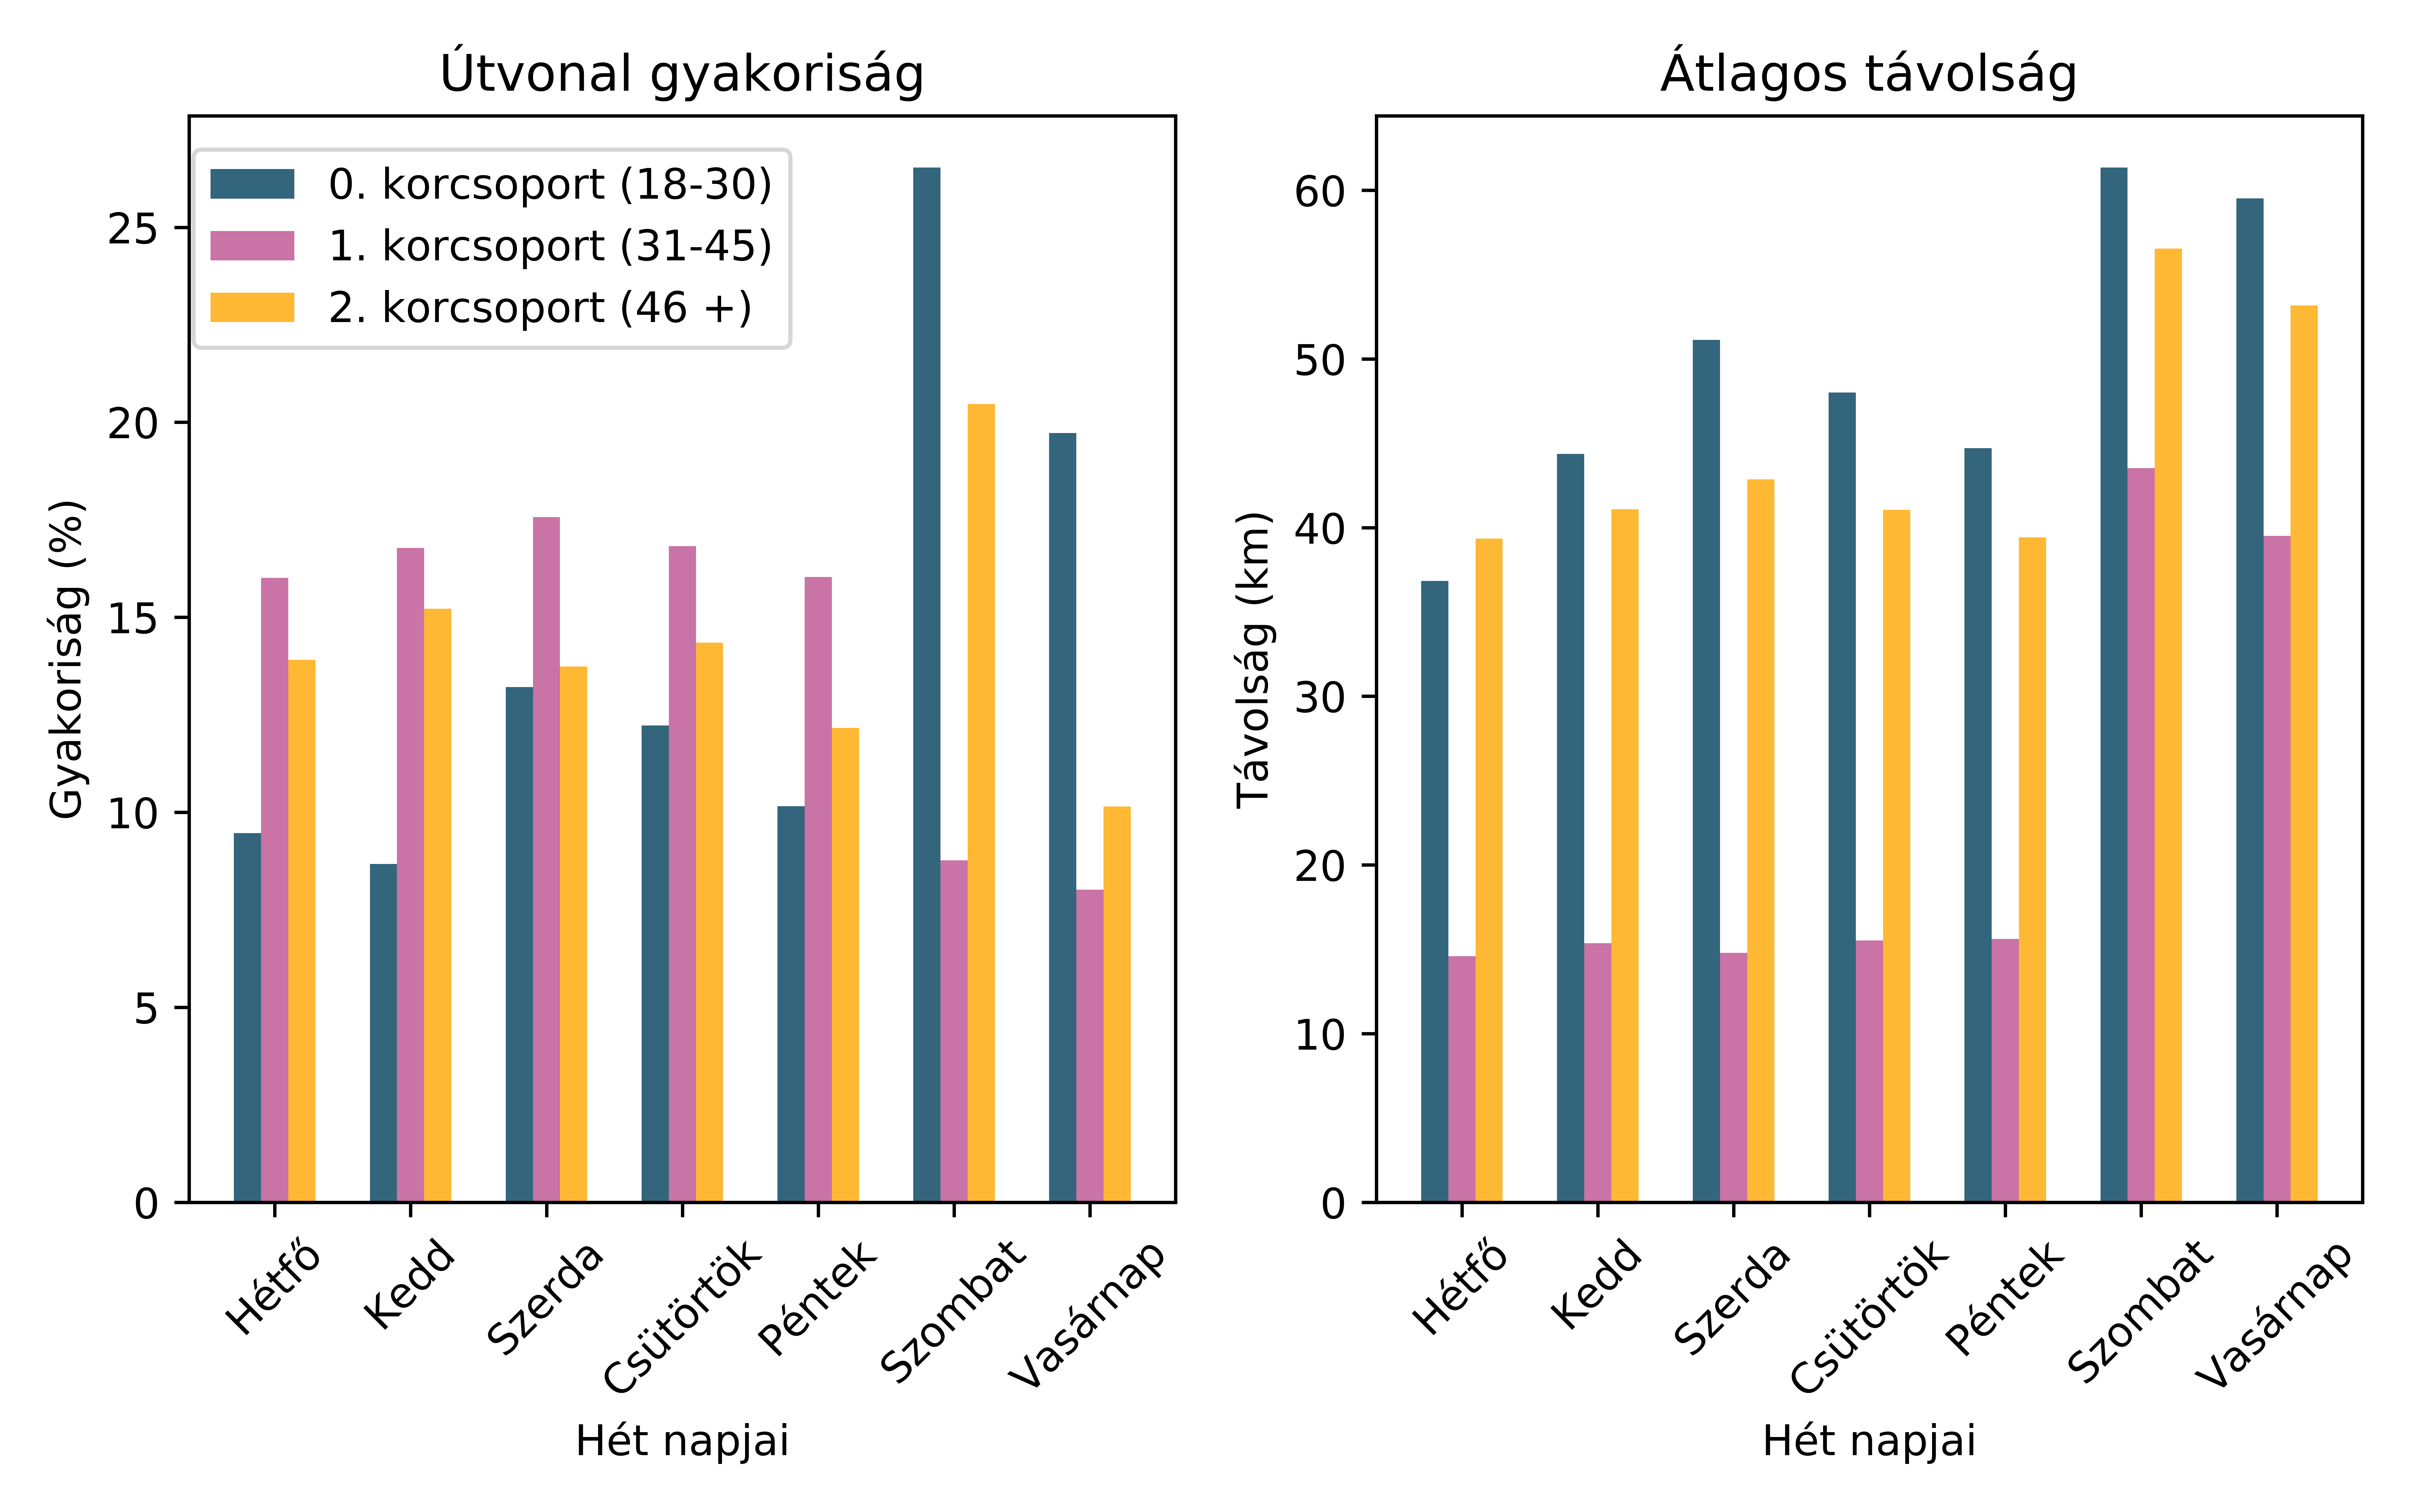
\includegraphics[width=\linewidth,keepaspectratio]{kepek/data_insights/FrequencyAndDistanceOnWeekDays.png}
	\caption{Átlagos távolság és útvonal gyakoriság a hét napjain}
	\label{fig:distanceAndFrequencyByWeekdays}
\end{figure}



\begin{figure}
	\centering
	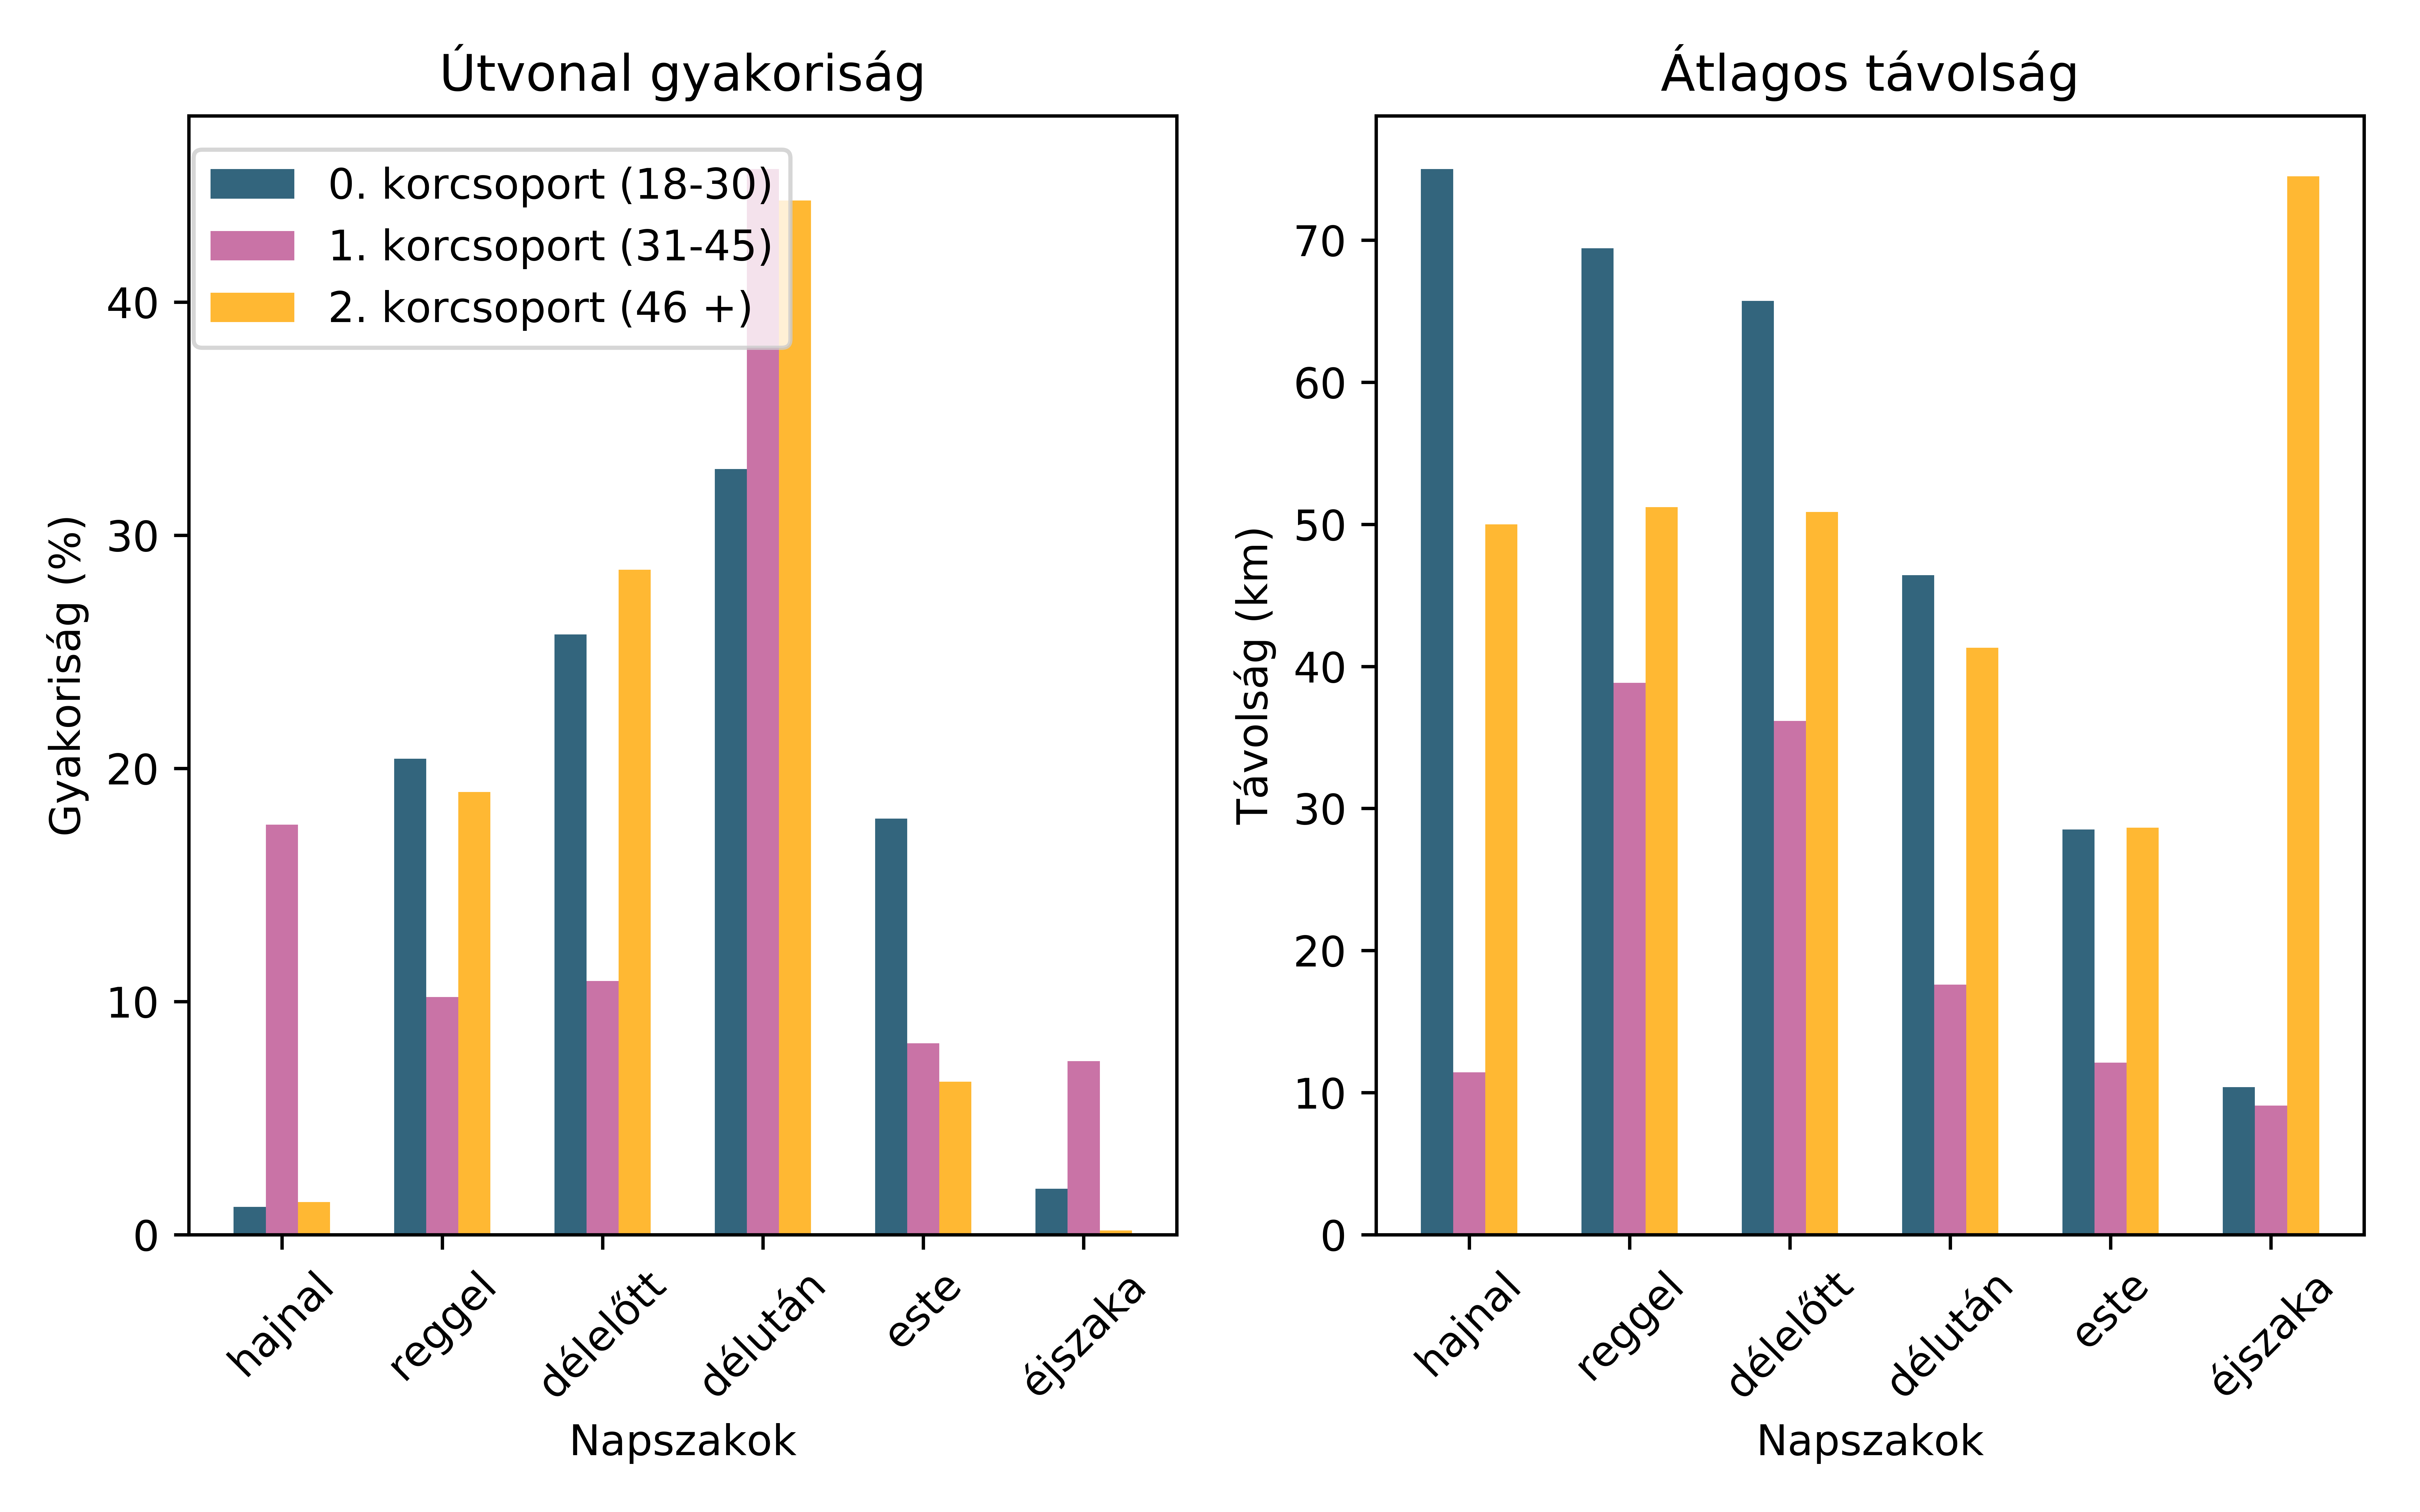
\includegraphics[width=\linewidth,keepaspectratio]{kepek/data_insights/FrequencyAndDistanceOnDayparts.png}
	\caption{Átlagos távolság és útvonal gyakoriság napszakok szerint}
	\label{fig:distanceAndFrequencyByDayparts}
\end{figure}


A \myref{fig:distanceAndFrequencyByWeekdays} ábrán két grafikon jellemzi az útvonalakat a hét napjai szerint. A bal oldali gráf az útvonalak darabszámának eloszlását jelzi, a jobb oldali pedig az átlagosan megtett távolságot, mindkét esetben korcsoportok szerint lebontva. Érdekesség hogy az 1. korcsoportba tartozó sportolók által megtett útvonalak nagyjából 80\%-a hétköznapra esik, azonban ezen útvonalak átlag távolsága mindössze 15 km körül mozog szemben a hétvégi kerékpározások átlagos 40 kilométerével. Természetesen minden korosztály esetén a hétvégén megemelkedik az átlagosan megtett távolság hiszen ilyenkor mindenkinek több ideje van nagyobb túrák teljesítésére. Hét közben nagy eltérés figyelhető meg az átlagos távolság esetében: az 1. korcsoportba tartozó kerékpározók messze elmaradnak a másik két korcsoportba tartozók mögött. Ennek egy lehetséges kiváltó oka hogy az 1. korcsoportban valószínűleg mindenki dolgozik, esetleg építkezik, családra koncentrál így érthetően kevesebb idejük van hosszú túrákra, valószínűleg munkába járás, közlekedés céljából kerékpároznak inkább hétköznapokon.


A \myref{fig:distanceAndFrequencyByDayparts} ábrán látható két grafikon az útvonalak gyakoriságát és az átlagosan megtett távolságot napszakokra lebontva jeleníti meg. A napszakok kialakítása szubjektív módon, a \myref{fig:daypartsClock} ábrán található 24 órás lebontás alapján történt. 


\begin{figure}[!h]
	\centering
	\begin{tikzpicture}[line cap=rect,line width=3pt]
	\filldraw[fill=chart5, draw=chart5, line width=1pt] (0,0)-- +(45:2) arc (45:0:2); %hajnal
	\filldraw[fill=chart0, draw=chart0, line width=1pt] (0,0)-- +(120:2) arc (120:45:2); %éjszaka
	\filldraw[fill=chart1, draw=chart1, line width=1pt] (0,0)-- +(180:2) arc (180:120:2); %este
	\filldraw[fill=chart2, draw=chart2, line width=1pt] (0,0)-- +(270:2) arc (270:180:2); %délután
	\filldraw[fill=chart3, draw=chart3, line width=1pt] (0,0)-- +(315:2) arc (315:270:2); %délelőtt
	\filldraw[fill=chart4, draw=chart4, line width=1pt] (0,0)-- +(360:2) arc (360:315:2); %reggel
	
	\node[font=\small] at (90:2.36cm) {\textsf{Éjszaka}};
	\node[font=\small] at (20:2.7cm) {\textsf{Hajnal}};
	\node[font=\small] at (340:2.7cm) {\textsf{Reggel}};
	\node[font=\small] at (305:2.6cm) {\textsf{Délelőtt}};
	\node[font=\small] at (215:2.7cm) {\textsf{Délután}};
	\node[font=\small] at (155:2.6cm) {\textsf{Este}};
	
	\draw (0,0) circle [radius=2cm];
	
	\foreach \angle [count=\xi] in {75,60,...,-270}
	{
		\draw[line width=1pt] (\angle:1.8cm) -- (\angle:2cm);
		%\node[font=\small] at (\angle:1.36cm) {\textsf{\xi}};
	}
	\foreach \angle [count=\xi] in {0,45,90,135,180,225,270,315}
	{
		\draw[line width=2pt] (\angle:1.6cm) -- (\angle:2cm);
	}
	\draw (0,0) -- (120:0.8cm);
	\draw (0,0) -- (90:1cm);
	\node[font=\small] at (0:1.36cm) {\textsf{6}};
	\node[font=\small] at (45:1.36cm) {\textsf{3}};
	\node[font=\small] at (90:1.36cm) {\textsf{0}};
	\node[font=\small] at (135:1.30cm) {\textsf{21}};
	\node[font=\small] at (180:1.36cm) {\textsf{18}};
	\node[font=\small] at (225:1.36cm) {\textsf{15}};
	\node[font=\small] at (270:1.36cm) {\textsf{12}};
	\node[font=\small] at (315:1.36cm) {\textsf{9}};
	
	
	%\filldraw[line color=gray!40 ] -- +(45:2) arc (45:-45:2);
	\end{tikzpicture}
	\caption{Napszakok kialakítása}
	\label{fig:daypartsClock}
\end{figure}



\SubSection{További adat feldolgozás}

\subsubsection{One-hot encoding}
A kiugró értékek kezelése és a adathalmaz összefüggéseinek vizsgálata után a következő lépés a one-hot encoding. Az eljárás lényege hogy egy kategória alapú jellemzőt több (a kategóriák számának megfelelő) oszlopra bont szét, ahol az egyes oszlopokban, jellemzőkben 1-es szerepel amennyiben az adatsor abba az adott kategóriába sorolható, 0 egyébként. Ennek az előnye hogy kiküszöböli a kategóriák sorszámmal történő jelzésének távolságát. Például egy korcsoportot tároló jellemző esetén nem biztos hogy helyes feltételezni hogy a 0. és a 2. kategória (csoport) között 2 távolság van. A one hot encoding természetesen folytonos változók esetén nem értelmezhető és kategoriális jellemzőkre sem mindig érdemes alkalmazni.

A szakdolgozathoz használt adathalmaz esetén 3+1 jellemző kerül one-hot encode-olásra: age\_group (korcsoport), workout\_tpye, start\_date\_local és a training.\\[6pt]

\textbf{age\_group:} a sportoló korcsoportját jelzi, értékei egy három elemű halmazból kerülhetnek ki: \{0, 1, 2\} ahol 0 a [18, 30], 1 a [31, 45], 2 pedig a [46, $+\infty$) korcsoportokba való tartozást jelenti. One-hot encoding során az eredeti jellemzőből 3 oszlop készül, végül az eredeti törlésre kerül az adathalmazból.
\begin{programreszlet}
Python parancsok részletezése
\begin{python}
ageOneHot = pandas.get_dummies(rawData['age_group'], prefix='age')
rawData.drop(columns=['age_group'], inplace=True)
rawData = rawData.join(ageOneHot)
\end{python}
\end{programreszlet}
A kódban megadott prefix paraméter segítségével az új jellemzők nevei: age\_0.0, age\_1.0, age\_2.0\\[6pt]


\textbf{workout\_tpye:} az aktivitás típusát jellemzi, értékei egy 3 elemű halmazból kerülhetnek ki: \{10, 11, 12\}, ahol 10: általános kerékpározás / jelöletlen; 11: verseny, 12: edzés. 

\begin{programreszlet} A \textit{workout\_type} kategorikus jellemző, így a számítások előtt One-hot encoding alkalmazásával lebontásra került az alábbi kód segítségével. 
\begin{python}
workoutTypeOneHot = pandas.get_dummies(rawData['workout_type'],
				       prefix='workout_type')
rawData.drop(columns='workout_type', inplace=True)
rawData = rawData.join(workoutTypeOneHot)
\end{python}
\end{programreszlet}


\textbf{start\_date\_local:} a jellemző az aktivitás kezdeti idejét tárolja, a sportoló saját időzónája szerint, ÉÉÉÉ-MM-DD HH:MM:SS formátumban. Dátum mezők azonban nem értelmezhetőek gépi tanulási algoritmusokkal így a jellemző átalakítása szükségszerű volt. A dátumból alapvetően 2 féle új jellemző kerül kinyerésre, majd ezek külön kerülnek one-hot encode-olásra

\begin{programreszlet}
Az aktivitás kezdetének dátumából kinyerhető hogy a hét melyik napján történt az aktivitás. Ezen információ kinyerését és one-hot encode-olását az alábbi kód végzi
\begin{python}
rawData['day_of_week'] = rawData['start_date_local'].dt.day_name()
weekDayOneHot = pandas.get_dummies(rawData['day_of_week'], 
				   prefix='weekday')
rawData.drop(columns=['day_of_week'], inplace=True)
rawData = rawData.join(weekDayOneHot)
\end{python}		
\end{programreszlet}

\begin{programreszlet}
Az aktivitás kezdetének időpontjából kinyerhető hogy melyik napszakban kezdődött az aktivitás. Ezen információ kinyerését és one-hot encode-olását az alábbi kód végzi
\begin{python}
rawData['daypart'] = rawData['start_date_local'].apply(lambda row: 
						 timeToPartOfDay(row))
dayPartOneHot = pandas.get_dummies(rawData['daypart'], prefix='daypart')
rawData.drop(columns=['daypart'], inplace=True)
rawData = rawData.join(dayPartOneHot)
\end{python}	

Ahol a \textit{timeToPartOfDay} függvény a \textit{start\_date\_local} jellemző minden adattagjára külön hívódik meg. Ez a függvény szubjektíven oszt fel egy napot hat napszakra \myaref{fig:daypartsClock} ábra szerint

\end{programreszlet}



\textbf{trainer: } a trainer jellemző Igaz / Hamis értékekkel jelzi hogy egy adott aktivitás traineren, azaz gépen történt e, nem pedig tényleges kerékpáron. Ennek a jellemzőnek az átalakítása nem igazi one-hot encoding, inkább csak az Igaz / Hamis értékek átalakítása 1 / 0 értékekre.  


Az adattisztítás összes lépése után az adathalmaz szerkezete lényegesen megváltozik, új jellemzőket tartalmaz (one-hot encoding) valamint az eddigi jellemzők sok esetben más intervallumokba esnek (kiugró értékek kezelése).

Jellemzők:
\begin{itemize}
	\item average\_speed: átlagsebesség az útvonal során (méter / másodperc)
	\item distance: összesen megtett távolság (méter)
	\item elapsed\_time: összesen eltelt idő (másodperc)
	\item elev\_high: útvonal legmagasabb pontja (méter)
	\item elev\_low: útvonal legalacsonyabb pontja (méter)
	\item hashed\_id: sportoló hashelt azonosítója
	\item max\_speed: legnagyobb elért sebesség (méter / másodperc)
	\item moving\_time: mozgással töltött idő (másodperc)
	\item total\_elevation\_gain: összesen megtett emelkedés (méter)
	\item age\_0.0: 0. korcsoportba való tartozást jelöli (bináris)
	\item age\_1.0: 1. korcsoportba való tartozást jelöli (bináris)
	\item age\_2.0: 2. korcsoportba való tartozást jelöli (bináris)
	\item trainer\_onehot: útvonal megtétele gépen történt e (bináris)
	\item workout\_type\_10.0: 10 típusú útvonal (bináris)
	\item workout\_type\_11.0: 11 típusú útvonal (bináris)
	\item workout\_type\_12.0: 12 típusú útvonal (bináris)
	\item weekday\_Monday: hétfői aktivitás (bináris)
	\item weekday\_Tuesday: keddi aktivitás (bináris)
	\item weekday\_Wednesday: szerdai aktivitás (bináris)
	\item weekday\_Thursday: csütörtöki aktivitás (bináris)
	\item weekday\_Friday: pénteki aktivitás (bináris)
	\item weekday\_Saturday: szombati aktivitás (bináris)
	\item weekday\_Sunday: vasárnapi aktivitás (bináris)
	\item daypart\_dawn: hajnali indulás (bináris)
	\item daypart\_morning: reggeli indulás (bináris)
	\item daypart\_forenoon: délelőtti indulás (bináris)
	\item daypart\_afternoon: délutáni indulás (bináris)
	\item daypart\_evening: esti indulás (bináris)
	\item daypart\_night: éjszakai indulás (bináris)
\end{itemize}


Az adathalmaz ezen a ponton mentésre kerül a későbbi felhasználás megkönnyítésének céljából. A tisztított adatot a \textit{cleaned\_data\_\{date\}.csv} fájl tartalmazza.


A tisztított adathalmaz numerikus oszlopainak összefoglalása a \myref{tab:cleanDataDescription} táblázatban található.

% Please add the following required packages to your document preamble:
% \usepackage{graphicx}
% Please add the following required packages to your document preamble:
% \usepackage{graphicx}
\begin{table}[!h]
	\resizebox{\textwidth}{!}{%
		\begin{tabular}{l|l|l|l|l|l|l|l|l|}
			\cline{2-9}
			& \textbf{count} & \textbf{mean} & \textbf{std} & \textbf{min} & \textbf{0.25} & \textbf{0.50} & \textbf{0.75} & \textbf{max} \\ \hline
			\multicolumn{1}{|l|}{\textbf{average\_speed}}                                                    & 9603           & 5.76          & 1.22         & 2.03         & 4.99          & 5.74          & 6.46          & 12.48        \\ \hline
			\multicolumn{1}{|l|}{\textbf{distance}}                                                          & 9603           & 26140.85      & 29199.25     & 161.0        & 7451.3        & 13702.2       & 34599.1       & 436806.0     \\ \hline
			\multicolumn{1}{|l|}{\textbf{elapsed\_time}}                                                     & 9603           & 5817.39       & 19632.69     & 61.0         & 1645.0        & 2998.0        & 7338.5        & 1806211.0    \\ \hline
			\multicolumn{1}{|l|}{\textbf{elev\_high}}                                                        & 9603           & 270.73        & 166.61       & -71.2        & 162.3         & 229.4         & 290.5         & 956.0        \\ \hline
			\multicolumn{1}{|l|}{\textbf{elev\_low}}                                                         & 9603           & 129.92        & 47.88        & -134.4       & 103.2         & 130.2         & 148.3         & 809.6        \\ \hline
			\multicolumn{1}{|l|}{\textbf{max\_speed}}                                                        & 9603           & 12.22         & 3.24         & 2.3          & 9.7           & 11.6          & 14.4          & 22.0         \\ \hline
			\multicolumn{1}{|l|}{\textbf{moving\_time}}                                                      & 9603           & 4509.68       & 4948.21      & 61.0         & 1440.0        & 2415.0        & 6099.0        & 90983.0      \\ \hline
			\multicolumn{1}{|l|}{\textbf{\begin{tabular}[c]{@{}l@{}}total\_elevation\\ \_gain\end{tabular}}} & 9603           & 274.47        & 410.03       & 0.0          & 29.8          & 87.0          & 359.45        & 3896.8       \\ \hline
		\end{tabular}%
	}
\caption{Tisztított adathalmaz numerikus oszlopai}
\label{tab:cleanDataDescription}
\end{table}


% ADATTISZTITAS VEGE


% ML KEZDETE

\Section{Regresszió}
Az adathalmaz egy aktivitásra tekintve két különböző időtartamot különböztet meg: a mozgással töltött (\textit{moving\_time}) és az összesen eltelt (\textit{elapsed\_time}) időt, mindkettőt másodpercben mérve. 
Ennek a két időtartamnak a becslése a \myref{subsec:regression} alfejezetben kifejtett regressziók felhasználásával történik.

A kétféle időtartam alapvetően külön kezelve, egyenként kerül becslésre.

\SubSection{Paraméter hangolás}
A gépi tanulási algoritmusok tanításának eredményessége kis mértékben javítható az adott eljárás paramétereinek a használt adathalmazhoz való igazításával. Az algoritmusok a scikit-learn megvalósításában rendelkeznek alapparaméterekkel, tehát egy alapvető eredmény ezek explicit beállítása nélkül is számítható, azonban a megfelelő paraméterek kiválasztása akár néhány százalékos javulást is eredményezhet.

%A szakdolgozat során ennek a két időtartamnak a várható értékének a meghatározása az egyik cél gépi tanulási algoritmusokkal valamint ezen algoritmusoknak az összehasonlítása. Ennek a feladatnak a megoldásához a  \myref{subsec:regression} alfejezetben kifejtett regressziók adnak alapot.


\subsubsection{Ridge regresszió:} ez az algoritmus 2 fő paraméterrel finomhangolható: $\alpha \geq 0 $ és \textit{solver} $\in$ \{auto, svd, cholesky, lsqr, sparce\_cg, sag, saga\}. Az $\alpha$ paraméter a regularizáció mértékét befolyásolja a különböző \textit{solver}-ek pedig a számítási rutint befolyásolják (lsd.: dokumentáció). Az algoritmus optimalizálása során $\alpha \in$ \{0.0001, 0.0003, 0.001, 0.003, 0.01, 0.1, 0.3, 0.35, 0.6\} értékek kerültek figyelembe vételre.\\[6pt]

\subsubsection{Lasso regresszió:} a modell finomhangolása elsősorban az $\alpha \geq 0$ paraméter változtatásával történik. A scikit-learn implementáció lehetőséget ad egyéb opciók beállítására azonban ezek nem befolyásolják nagyban a modell működését így használatuk mellőzésre kerül a szakdolgozat során. Az optimalizálás során $\alpha \in$ \{0.0001, 0.0003, 0.001, 0.003, 0.01, 0.1, 0.3, 0.35, 0.6\} értékek kerültek figyelembe vételre.\\[6pt]

\subsubsection{Random Forest regresszió:} ez a döntési fákon alapuló eljárás lényegesen mélyebben személyre szabható a paraméterei révén mint a Ridge és a Lasso regresszió. Optimalizálása \cite{random-forest-tuning} során a következő paraméterek kerültek felhasználásra:
\begin{itemize}
	\item n\_estimators$\in$ \{200, 500, 1000\}: fák száma
	\item max\_features $\in$ \{auto, sqrt\}: a legjobb felosztás megtalálásához felhasználandó jellemzők darabszáma
	\item min\_samples\_leaf $\in$ \{10, 30, 60\}: egy levél legalább hány mintát tartalmazzon
\end{itemize}
A Random Forest egyéb paraméterei is befolyásolhatják a tanulás eredményességét, a becslések pontosságát. 

A tanítás előtt elő kell készíteni az adattisztítást eredményeként kapott ömlesztett adathalmazt. Ennek első lépése a magyarázó $X$ és a függő $y$ halmazok kialakítása. Ezeknek változniuk kell annak függvényében hogy a mozgással töltött időt vagy az összesen eltelt idő becslése e a cél aktuálisan. Azonban miután kialakításra kerül a két adathalmaz fontos hogy a regressziós modellek tanítása előtt standardizálásra kerüljenek. Ennek fontossága akkor mutatkozik meg igazán mikor a különböző jellemzők nagyon eltérő intervallumokba esnek, például a \textit{average\_speed} 2.03 és 12.478 értékek között mozog, míg a \textit{distance} jellemző 161 és 436806 között. A standardizálás elvégzésére a szakdolgozat során a scikit-learn csomag által biztosított StandardScaler függvény szolgál.
\begin{programreszlet} 	Adathalmaz általános standardizálása
\begin{python}
from sklearn.preprocessing import StandardScaler
def getStandardized(X):
    X = dataset.copy()
	
    names = X.columns
    scaler = StandardScaler()
		
    scaledData = scaler.fit_transform(X)
    scaledData = pandas.DataFrame(scaledData, columns=names)
    return scaledData
\end{python}
\label{prog:movingStandard}
\end{programreszlet}

\begin{programreszlet} A túltanulás elkerülése érdekében a tanító és cél adathalmazokat szét kell osztani tanító és tesztelő részekre. A regressziós modellek csak a tanító (\textit{train}) adatokon fognak tanulni, ellenőrzésre, pontosság meghatározására pedig a teszt (\textit{test}) adatok szolgálnak. A tanító és teszt adathalmazok kialakítására a scikit-learn csomag által biztosított \textit{train\_test\_split} függvény szolgál.
\begin{python}
from sklearn.model_selection import train_test_split
		
scaledY = scaledData['{target_feature}']
scaledData.drop(columns=['{target_feature}'], inplace=True)
		
trainX, testX, trainy, testy = train_test_split(scaledData, scaledY, 
						random_state=42)
\end{python}
\label{prog:movingTrainTestSplit}
\end{programreszlet}


\SubSection{Mozgási idő}
A mozgási idő becsléséhez három különböző adathalmaz kerül kialakításra:
\begin{itemize}
	\item \textit{all}: az $X$ halmaz a \textit{moving\_time} az \textit{elapsed\_time} és az \textit{average\_speed} oszlopok kivételével minden jellemzőt tartalmaz
	\item \textit{reduced}:  az $X$ halmazban csupán a következő jellemzők találhatóak meg:  \textit{age\_0.0}, \textit{age\_1.0}, \textit{age\_2.0}, \textit{distance}, \textit{elev\_high}, \textit{elev\_low}, \textit{hashed\_id}, \textit{total\_elevation\_ gain}, \textit{trainer\_onehot}
	\item \textit{base}: az $X$ halmaz kizárólag az útvonal fizikai jellemzőit tartalmazza: \textit{distance}, \textit{elev\_high},\textit{elev\_low}, \textit{total\_elevation\_gain}, \textit{trainer\_onehot}, \textit{text}.
\end{itemize}
Mindkét adathalmaz esetén $y$ csak a \textit{moving\_time} jellemzőt tartalmazza és természetesen megtörténik az adatok standardizálása valamint tanító és tesztelő részhalmazokra való bontása a \myref{prog:movingStandard} és a \myref{prog:movingTrainTestSplit} programrészletek segítségével.


\subsubsection{Eredmények}

A Ridge és Lasso regresszió eredményei a \myref{table:movingTimeRidgeAndLasso} táblázatban kerülnek összefoglalásra. Mint látható a két különböző modell szinte identikus pontosságot ad a teszt adathalmazokra, minimális csökkenéssel a \textit{reduced} X esetén. 
\begin{table}[!h]
	\centering
	\begin{tabular}{|l|r|r|r|r|c|}
		\hline
		\textbf{Modell} & \textbf{X} & \textbf{y}   & \multicolumn{1}{l|}{\textbf{Pontosság}} & \textbf{$\boldsymbol\alpha$} & \multicolumn{1}{l|}{\textbf{Solver}} \\ \hline
		\textbf{Ridge}  & all        & moving\_time & 0.935588                                & 0.3              & saga                                 \\ \hline
		\textbf{Ridge}  & reduced    & moving\_time & 0.933802                                & 0.1              & sag                                 \\ \hline
		\textbf{Ridge}  & base    & moving\_time & 0.920782                                  & 0.001              & sag                                  \\ \hline
		\textbf{Lasso}  & all        & moving\_time & 0.935583                                & 0.0001            & --                                   \\ \hline
		\textbf{Lasso}  & reduced    & moving\_time & 0.933784                                & 0.0001            & --                                   \\ \hline
		\textbf{Lasso}  & base    & moving\_time & 0.920763                                  & 0.0001            & --                                   \\ \hline
	\end{tabular}
	\caption{Ridge és Lasso eredmények moving\_time jellemző becslésére}
	\label{table:movingTimeRidgeAndLasso}
\end{table}

A Ridge és Lasso regressziók működése nagyon közel áll egymáshoz, csupán regularizáció tekintetében különböznek, így nem meglepő hogy a két módszer hasonló pontossággal ad becsléseket.\\[6pt]

\noindent A Random Forest regresszió eredményei a \myref{table:movingTimeRandomForest} táblázatban kerülnek összefoglalásra. Ez a döntési fákon alapuló eljárás alapjaiban különbözik a Ridge és Lasso regresszióktól azonban a szakdolgozatban használt adathalmazon közel azonos pontossággal teljesít. Általában 2-3\%-al ad rosszabb eredményeket mint a Ridge és Lasso regressziók.

% Please add the following required packages to your document preamble:
% \usepackage{graphicx}
\begin{table}[!h]
	\centering
	\resizebox{\textwidth}{!}{%
		\begin{tabular}{|r|r|c|r|r|}
			\hline
			\textbf{X}       & \textbf{Pontosság} & \textbf{max\_features} & \textbf{min\_samples\_leaf} & \textbf{n\_estimators} \\ \hline
			all     & 0.910675           & auto                   & 10                          & 500                    \\ \hline
			reduced & 0.908003           & auto                   & 10                          & 500                    \\ \hline
			base    & 0.894923           & auto                   & 10                          & 200                    \\ \hline
		\end{tabular}%
	}
	\caption{Random Forest regresszió eredmények \textit{moving\_time} jellemző becslésére}
	\label{table:movingTimeRandomForest}
\end{table}




\subsubsection{Összefoglalás}
A mozgási idő (\textit{moving\_time}) jellemző szorosan összefügg az útvonalak fizikai tulajdonságaival ezért egyszerű regressziókkal is nagy pontossággal becsülhető. Azonban a \myref{table:movingTimeRidgeAndLasso} és a \myref{table:movingTimeRandomForest} táblázatokban látható hogy csak az útvonal fizikai adatai alapján (\textit{base} adathalmaz) elért pontosság javítható egyéb, a sportolóhoz és időponthoz kapcsolható adatok segítségével. Ez alapján 
egyéb adatok segítségével (sportolóhoz, időponthoz kapcsolódó) a modellek finomhangolhatóak, nagyobb pontosság érhető el. 



\SubSection{Összesen eltelt idő}
A \myref{prog:movingStandard} és a \myref{prog:movingTrainTestSplit} program részletek segítségével 7 különböző adathalmaz kerül kialakításra. A cél mindig az \textit{elapsed\_time} jellemző becslése amelyet egyik $X$ sem tartalmaz
\begin{itemize}
	\item \textbf{all:} X minden jellemzőt tartalmaz 
	\item \textbf{reduced:} X csökkentett számú jellemzőt tartalmaz, név szerint a következőket: \textit{age\_0.0}, \textit{age\_1.0}, \textit{age\_2.0}, \textit{distance}, \textit{elev\_high}, \textit{elev\_low}, \textit{hashed\_id}, \textit{total\_elevation\_gain}, \textit{moving\_time}, \textit{trainer\_onehot}
	\item \textbf{ageNull:} X és y is csak a 0 korcsoportba (18-30) tartozó sportolók adatait tartalmazza 
	\item \textbf{ageOne:} X és y is csak az 1 korcsoportba (31-45) tartozó sportolók adatait tartalmazza
	\item \textbf{ageTwo:} X és y is csak a 2 korcsoportba (46+) tartozó sportolók adatait tartalmazza
	\item \textbf{distanceSmall:} X csak olyan útvonalakat tartalmaz ahol a távolság kisebb mint 50 km
	\item \textbf{distanceBig:} X csak olyan útvonalakat tartalmaz ahol a távolság nagyobb mint 50 km
	\item \textbf{user:} a legtöbb útvonallal rendelkező felhasználó adatait foglalja magába
	
\end{itemize}


\subsubsection{Eredmények}
A Ridge és Lasso regressziók eredményeit a \myref{table:elapsedTimeRidgeAndLasso} táblázat tartalmazza. Látható hogy az adat különböző részhalmazaira nagyon eltérő eredmények születtek, néhány esetben kiemelkedően rossz és meglepően jó pontosság is megfigyelhető. A mozgási idő kiegyensúlyozottságával szemben az eltelt időre a Lasso regresszió mindig jobban teljesít mint a Ridge. Általában csak 1\% körüli a teljesítmény különbség, de például a nagy távolságot tartalmazó adatok esetén (\textit{distanceBig}) 8\%-os különbség is megfigyelhető.
% Please add the following required packages to your document preamble:
% \usepackage{booktabs}
\begin{table}[h!]
	\centering
	\begin{tabular}{|r|c|r|r|c|}
		\hline
		\textbf{X}    & \textbf{Modell} & \multicolumn{1}{l|}{\textbf{Pontosság}} & \multicolumn{1}{l|}{\textbf{$\alpha$}} & \textbf{Solver} \\ \hline
		all           & Ridge           & 0.722601                                & 0.35                                   & lsqr            \\ \hline
		all           & Lasso           & 0.733696                                & 0.01                                   & --              \\ \hline
		reduced       & Ridge           & 0.741402                                & 0.6                                    & saga            \\ \hline
		reduced       & Lasso           & 0.742481                                & 0.001                                  & --              \\ \hline
		ageNull       & Ridge           & 0.922961                                & 0.003                                  & saga            \\ \hline
		ageNull       & Lasso           & 0.923146                                & 0.003                                  & --              \\ \hline
		ageOne        & Ridge           & 0.756610                                & 0.0                                    & auto            \\ \hline
		ageOne        & Lasso           & 0.774819                                & 0.01                                   & --              \\ \hline
		ageTwo        & Ridge           & 0.914806                                & 0.6                                    & saga            \\ \hline
		ageTwo        & Lasso           & 0.917202                                & 0.003                                  & --              \\ \hline
		distanceSmall & Ridge           & 0.325245                                & 0.6                                    & sag             \\ \hline
		distanceSmall & Lasso           & 0.384225                                & 0.01                                   & --              \\ \hline
		distanceBig   & Ridge           & 0.823487                                & 0.6                                    & saga            \\ \hline
		distanceBig   & Lasso           & 0.908215                                & 0.1                                    & --              \\ \hline
		user   & Ridge           & 0.184641                                & 0.6                                    & saga            \\ \hline
		user   & Lasso           & 0.184506                                & 0.6                                    & --              \\ \hline
	\end{tabular}
	\caption{Ridge és Lasso eredmények elapsed\_time becsléséhez}
	\label{table:elapsedTimeRidgeAndLasso}
\end{table}\\[6pt]

\noindent A Random Forest regresszió eredményei a \myref{table:elapsedTimeRandomForest} táblázat tartalmazza. A pontosságot összehasonlítva a \myref{table:elapsedTimeRidgeAndLasso} táblázatban lévő Ridge és Lasso regressziók pontosságával meglepő módon a Random Forest regresszió az esetek nagy részében jobban teljesít. Kivélelt a 0. és 2. korcsoportot (\textit{ageNull} és \textit{ageTwo}) valamint a nagy távolságú útvonalakat (\textit{distanceBig}) tartalmazó adathalmazok képeznek. A legnagyobb eltérés a felhasználói szintű adat (\textit{user}) esetén figyelhető meg: ez az adathalmaz összesen 2985 útvonalat tartalmaz (ezzel a teljes adathalmaz majdnem harmadát adva).

\begin{table}[!h]
	\centering
	\resizebox{\textwidth}{!}{%
		\begin{tabular}{|r|r|c|r|r|}
			\hline
			\textbf{X}    & \textbf{Pontosság} & \textbf{max\_features} & \textbf{min\_samples\_leaf} & \textbf{n\_estimators} \\ \hline
			all           & 0.813672           & sqrt                   & 10                          & 500                    \\ \hline
			reduced       & 0.812520           & sqrt                   & 10                          & 500                    \\ \hline
			ageNull       & 0.901840           & auto                   & 10                          & 200                    \\ \hline
			ageOne        & 0.779302           & sqrt                   & 10                          & 1000                   \\ \hline
			ageTwo        & 0.772750           & auto                   & 30                          & 500                    \\ \hline
			distanceSmall & 0.778130           & sqrt                   & 10                          & 1000                   \\ \hline
			distanceBig   & 0.902468           & auto                   & 10                          & 500                    \\ \hline
			user          & 0.839805           & auto                   & 10                          & 200                    \\ \hline
		\end{tabular}%
	}
\caption{Random Forest regresszió eredmények elapsed\_time jellemző becslésére}
\label{table:elapsedTimeRandomForest}
\end{table}



\subsubsection{Összefoglalás}
Az összesen eltelt idő ugyan összefügg az útvonalak fizikai adataival de nagy mértékben befolyásolják egyéb tényezők is. Így ennek a jellemzőnek a becslése lényegesen nehézkesebb mint a mozgással töltött időé. A eredmények alapján a kisebb, specifikusabb csoportokat tartalmazó adathalmazokra pontosabb becslések születtek. Például a korcsoport szerint lebontott adatok minden esetben nagyobb pontosságot eredményeztek mint az általános \textit{all} adathalmaz. Érdekes módon a \textit{reduced} $X$ használatakor mind a Ridge mind a Lasso regresszió eredményesebb volt mint az \textit{all} adathalmaz esetében. A legnagyobb kiingások a távolság szerint lebontott $X$-ek esetében található meg, valamint itt kell keresni a probléma magyarázatát is. Az 50 km-nél kettévágott (\textit{distance\_small} és \textit{distance\_big}) adatra készült becslések eredményei jól mutatják hogy a rövid útvonalaknál túl kevés az összefüggés ahhoz hogy pontos, használható modell készüljön belőle. Ennek oka hogy rövid távolság esetén egy specifikus felhasználó ismétlődő útvonalaira vetítve is változik az összesen eltelt idő, olyan befolyásoló tényezők hatására amiket az összegyűjtött adathalmaz nem tartalmaz, esetleg nem is mérhetőek. Ilyen tényezők lehetnek városi utak esetén a közlekedési lámpák, forgalom, néhány perces megállások felfrissülés, telefonálás vagy akár egy gyors bevásárlás miatt, és ezeken kívül természetesen rengeteg más. Hosszútávú útvonalak esetén azonban ezek közelebb eshetnek egymáshoz, általánosabb a kerékpározók pihenési ideje, az adathalmaz nem tartalmaz akkora variációkat mint a rövidebb útvonalak esetén. Ennek következtében a különböző regressziós módszerek sokkal jobban illeszkednek a hosszabb útvonalak esetén, jobb becsléseket adva a teszt adathalmaz elemeire.





\Section{Klaszterezés}
A gyűjtött adathalmaz nem tartalmaz nehézségre vonatkozó osztály címkéket, így felügyelet nélküli klaszterezés segítségével kerülnek kialakításra különböző csoportok. A klaszterezési eljárások különböző szabályok alapján csoportosítják az eredményeket, némelyik eljárásnál az eredmények minimálisan eltérhetnek a többszöri futtatáskor, aminek oka hogy a klaszter (csoport) középpontok véletlenszerűen inicializálódnak és előfordulhat hogy egy lokális minimumhoz konvergál az algoritmus.

A nehézségi csoportok meghatározásához az adathalmaz korcsoportok szerint  kerül felbontásra és ezeknek a részhalmazoknak csupán két jellemzője került felhasználásra: az átlagos sebesség (\textit{average\_speed}) és a távolság (\textit{distance}). Egy útvonalnak ez a két legalapvetőbb, atomi tulajdonsága, ami végső soron szinte minden másra kihatással van. Ezek a jellemzők mindhárom korcsoport esetén a \myref{ssec:klaszterezes} alfejezetben kifejtett K-Means, MiniBatch K-Means és Spectral klaszterezési módszerrel kerültek feldolgozásra. A cél 5 klaszter meghatározása, amelyek elkülönítésével és tulajdonságaik körbehatárolásával egy egyszerű edzésterv javaslatot adó rendszer készíthető el. 

%\TODO javaslat tevés leírása. Nagyon alapvető, később mindenképp továbbfejlesztésre szorul
A szakdolgozat során kidolgozott edzés tervező módszer egy nagyon alapvető számítás eredménye. A cél az egyes korcsoportokra különböző típusokat meghatározni és a típusokon belül eltérő nehézségű javaslatokat adni a felhasználók számára. Ennek megvalósításához a klaszterezési módszerekkel meghatározott típusokra külön - külön kerül kiszámításra az adott típusba tartozó adatok 25, 50 és 70\%-a, ezzel 3 nehézségi fokozatot meghatározva. Továbbá meghatározásra kerül a várható időtartam a kapott távolság és átlagos sebesség alapján. Ennek a módszernek a megvalósítása a \myref{prog:getTrainingSuggestion} programrészletben található.
\begin{programreszlet} Edzés javaslat számítása korcsoport (\textit{ageGroup}), klaszterezési algoritmus (\textit{clustering}), edzés típusa (\textit{trainType}) és nehézsége alapján (\textit{trainDifficulty}).
\begin{python}
def getTrainingSuggestions(self, ageGroup, clustering, trainType, 
			   trainDifficulty):
    if ageGroup == 0:
        data = self.ageNullInverted
    elif ageGroup == 1:
        data = self.ageOneInverted
    else:
        data = self.ageTwoInverted
        
    suggestion = data[data[clustering] == 
    		      trainType].quantile(trainDifficulty)
    # plotting suggestion
\end{python}
\label{prog:getTrainingSuggestion}
\end{programreszlet}
	
%Ehhez a klaszterezési módszerek segítségével meghatározott típusokhoz tartozó adatok 

\SubSection{0. korcsoport}
A részhalmaz összesen 914 útvonalat tartalmaz. A különböző klaszterezési eljárások eredményei a \myref{fig:clusteringAgeGroupNull} ábrán láthatóak. A kialakított klaszterek elhelyezkedése nagy vonalakban megegyezik, általánosan az alábbi módon lehetne jellemezni őket:
\begin{itemize}
	\item A : normális és nagy távolság - normális átlagsebesség
	\item B : nagy távolság - normális és magas átlagsebesség
	\item C : extrém nagy távolság - magas és extrém magas átlagsebesség
	\item D : normális távolság - magas átlagsebesség
	\item E : normális és nagy távolság - extrém magas átlagsebesség
\end{itemize}

\begin{figure}[!h]
	\centering
	\begin{subfigure}{.5\linewidth}
		\centering
		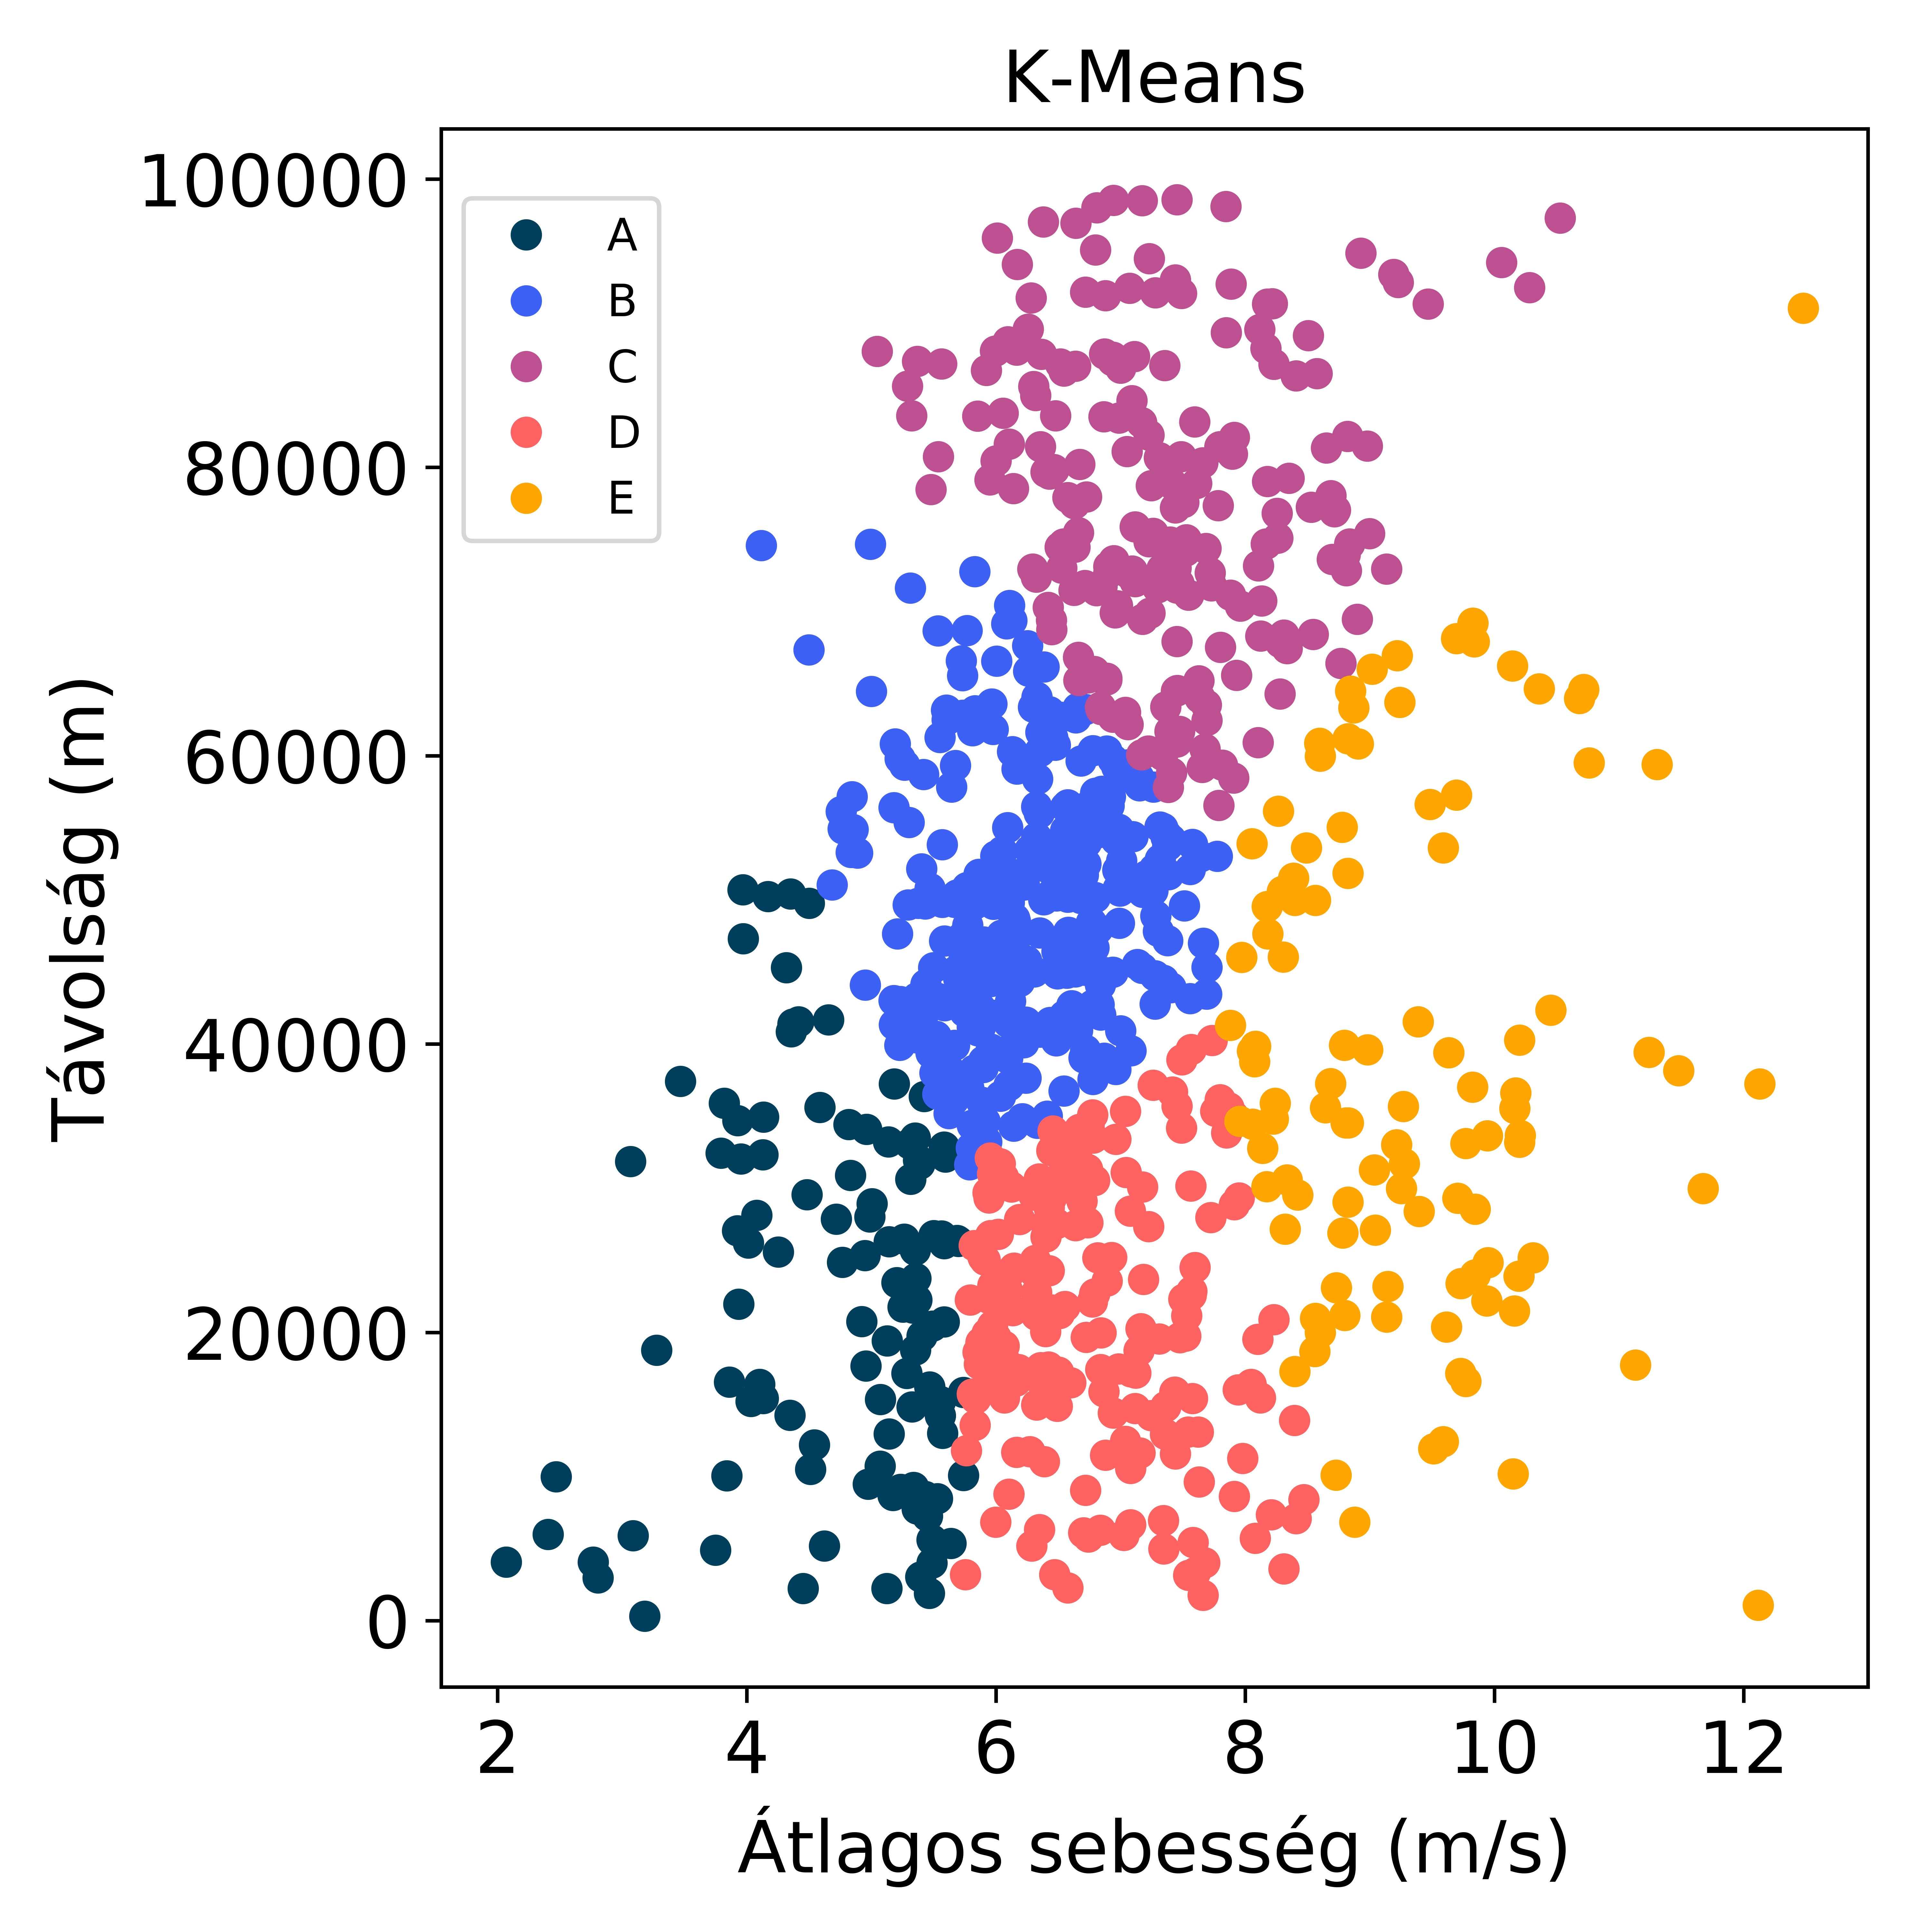
\includegraphics[width=\textwidth,keepaspectratio]{kepek/clustering/age_group_0_kmeans_results.png}
		\caption{K-Means}
		\label{subfig:clusteringAgeGroupNullKmeans}
	\end{subfigure}%
	\begin{subfigure}{.5\linewidth}
		\centering
		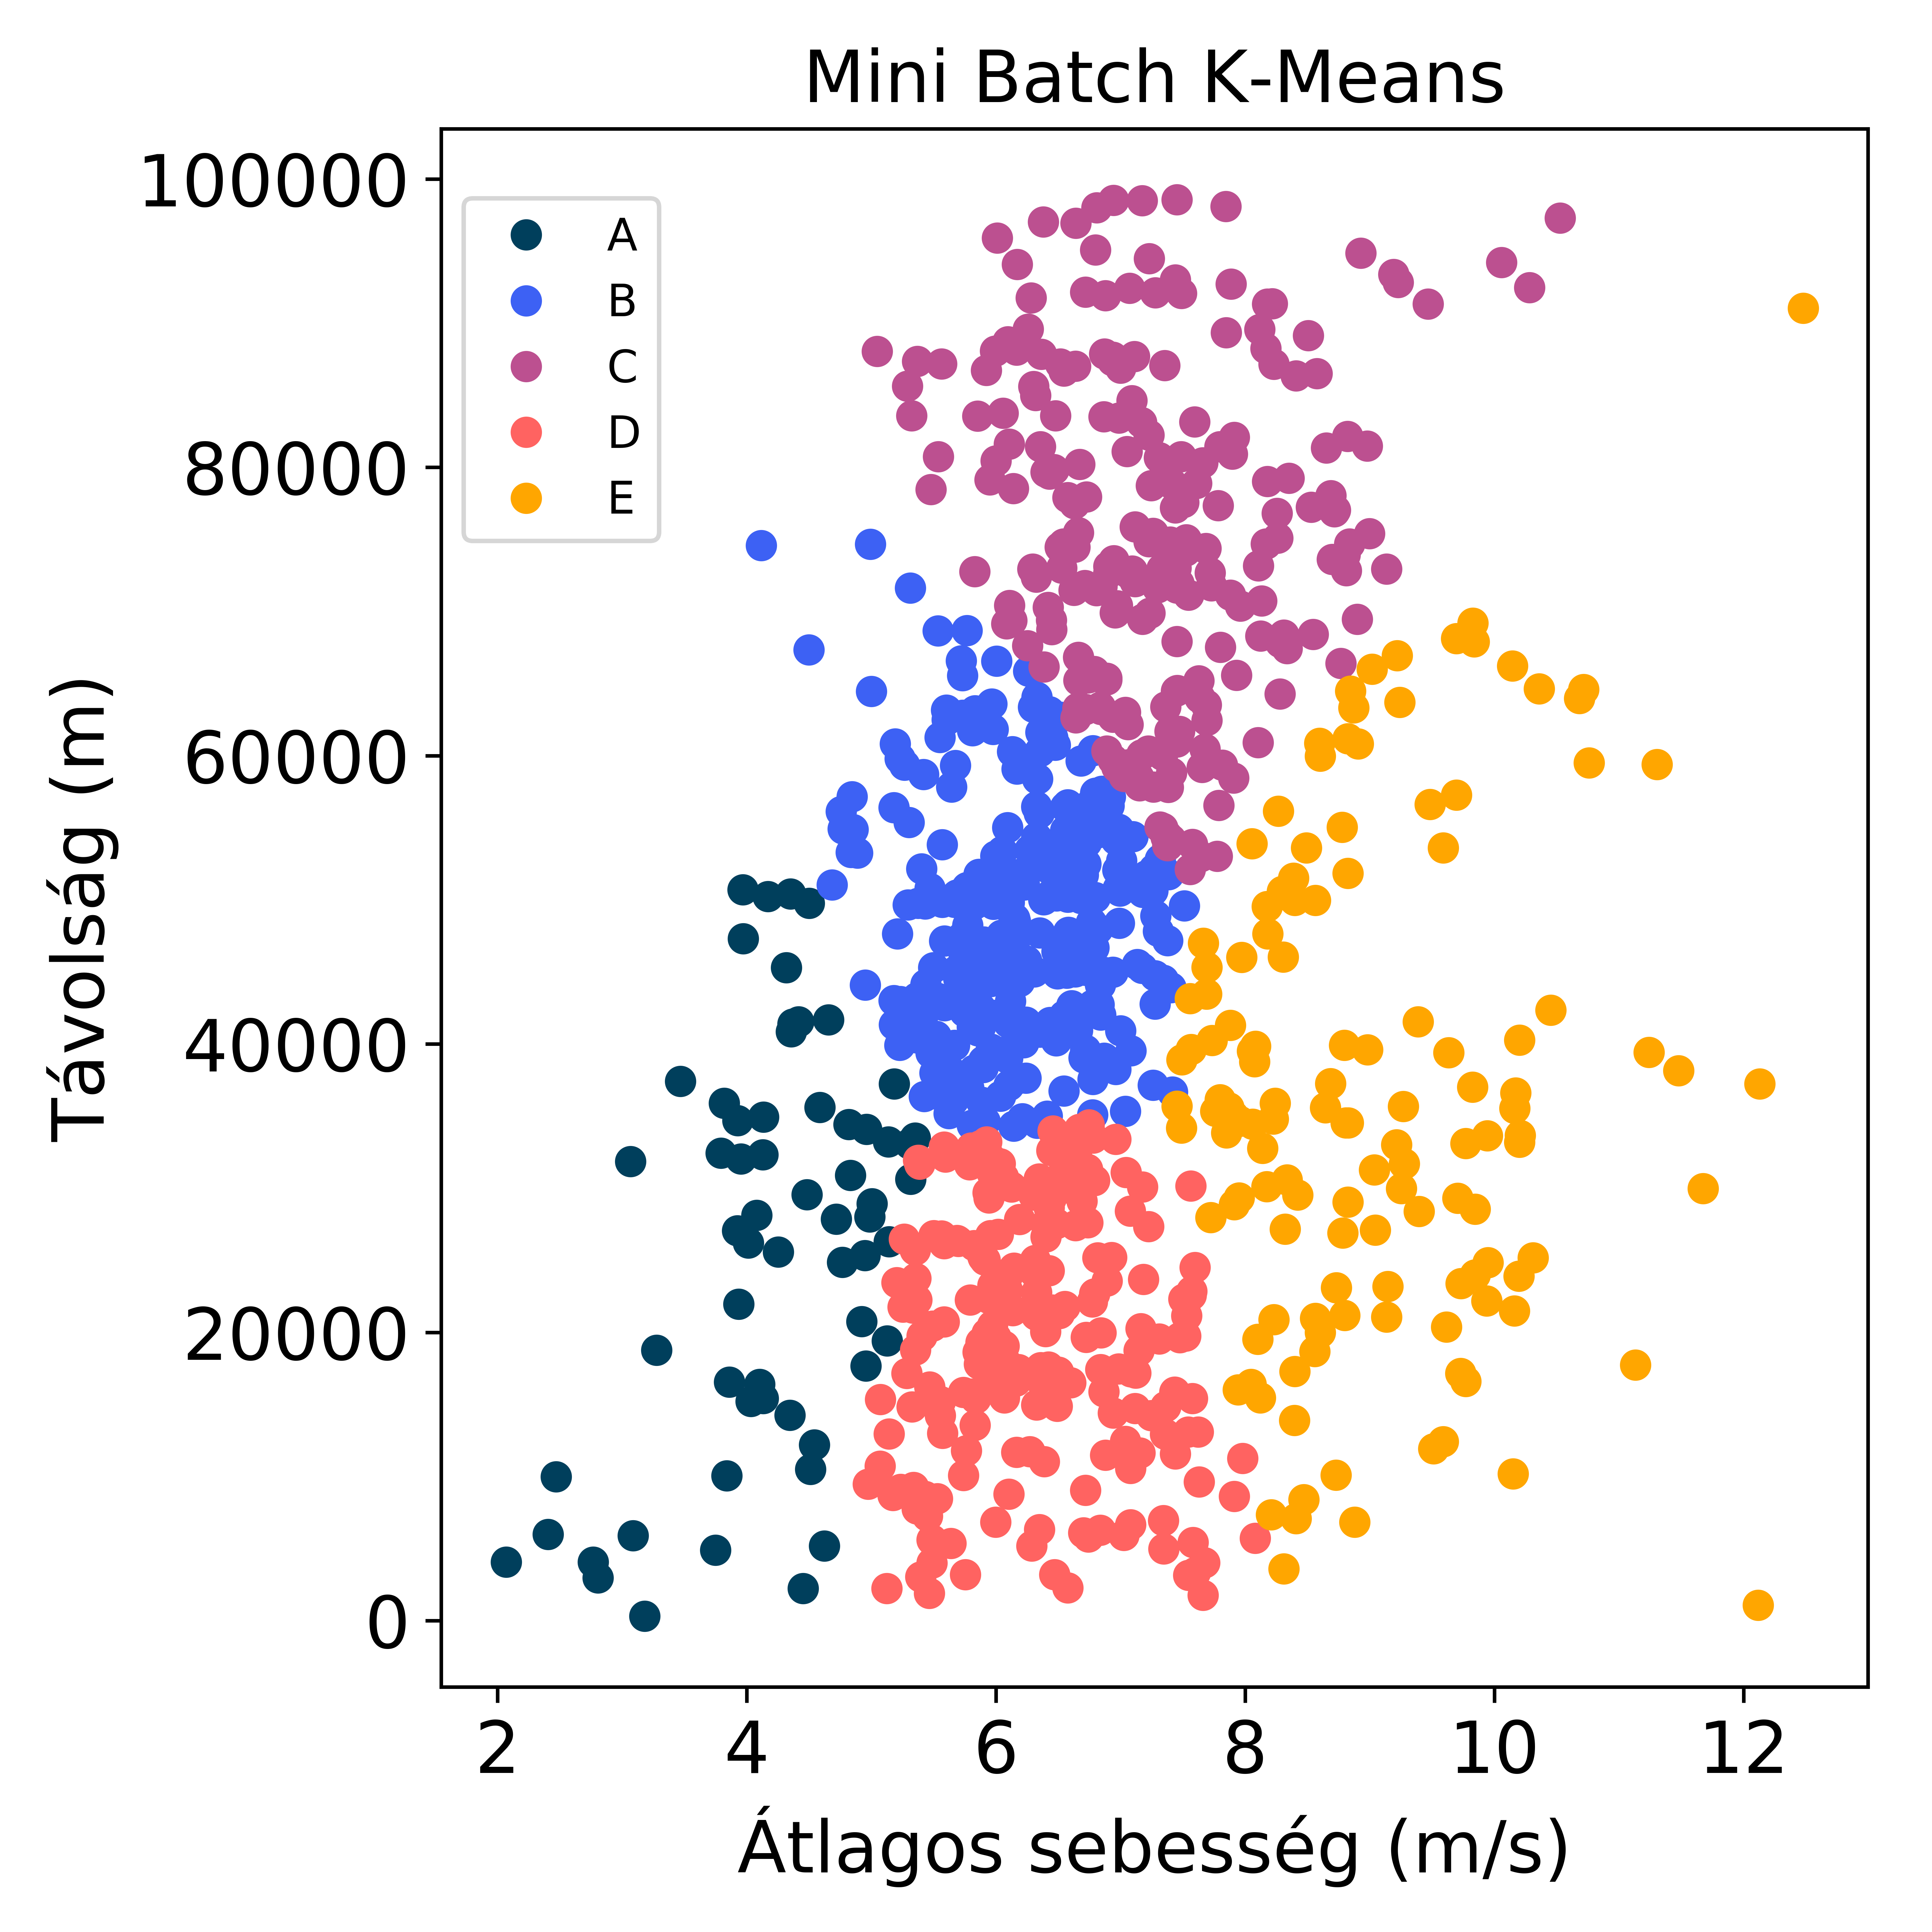
\includegraphics[width=\textwidth,keepaspectratio]{kepek/clustering/age_group_0_minibatch_results.png}
		\caption{Mini Batch K-Means}
		\label{subfig:clusteringAgeGroupNullMiniBatch}
	\end{subfigure}\\[1ex]
	\begin{subfigure}{.5\linewidth}
		\centering
		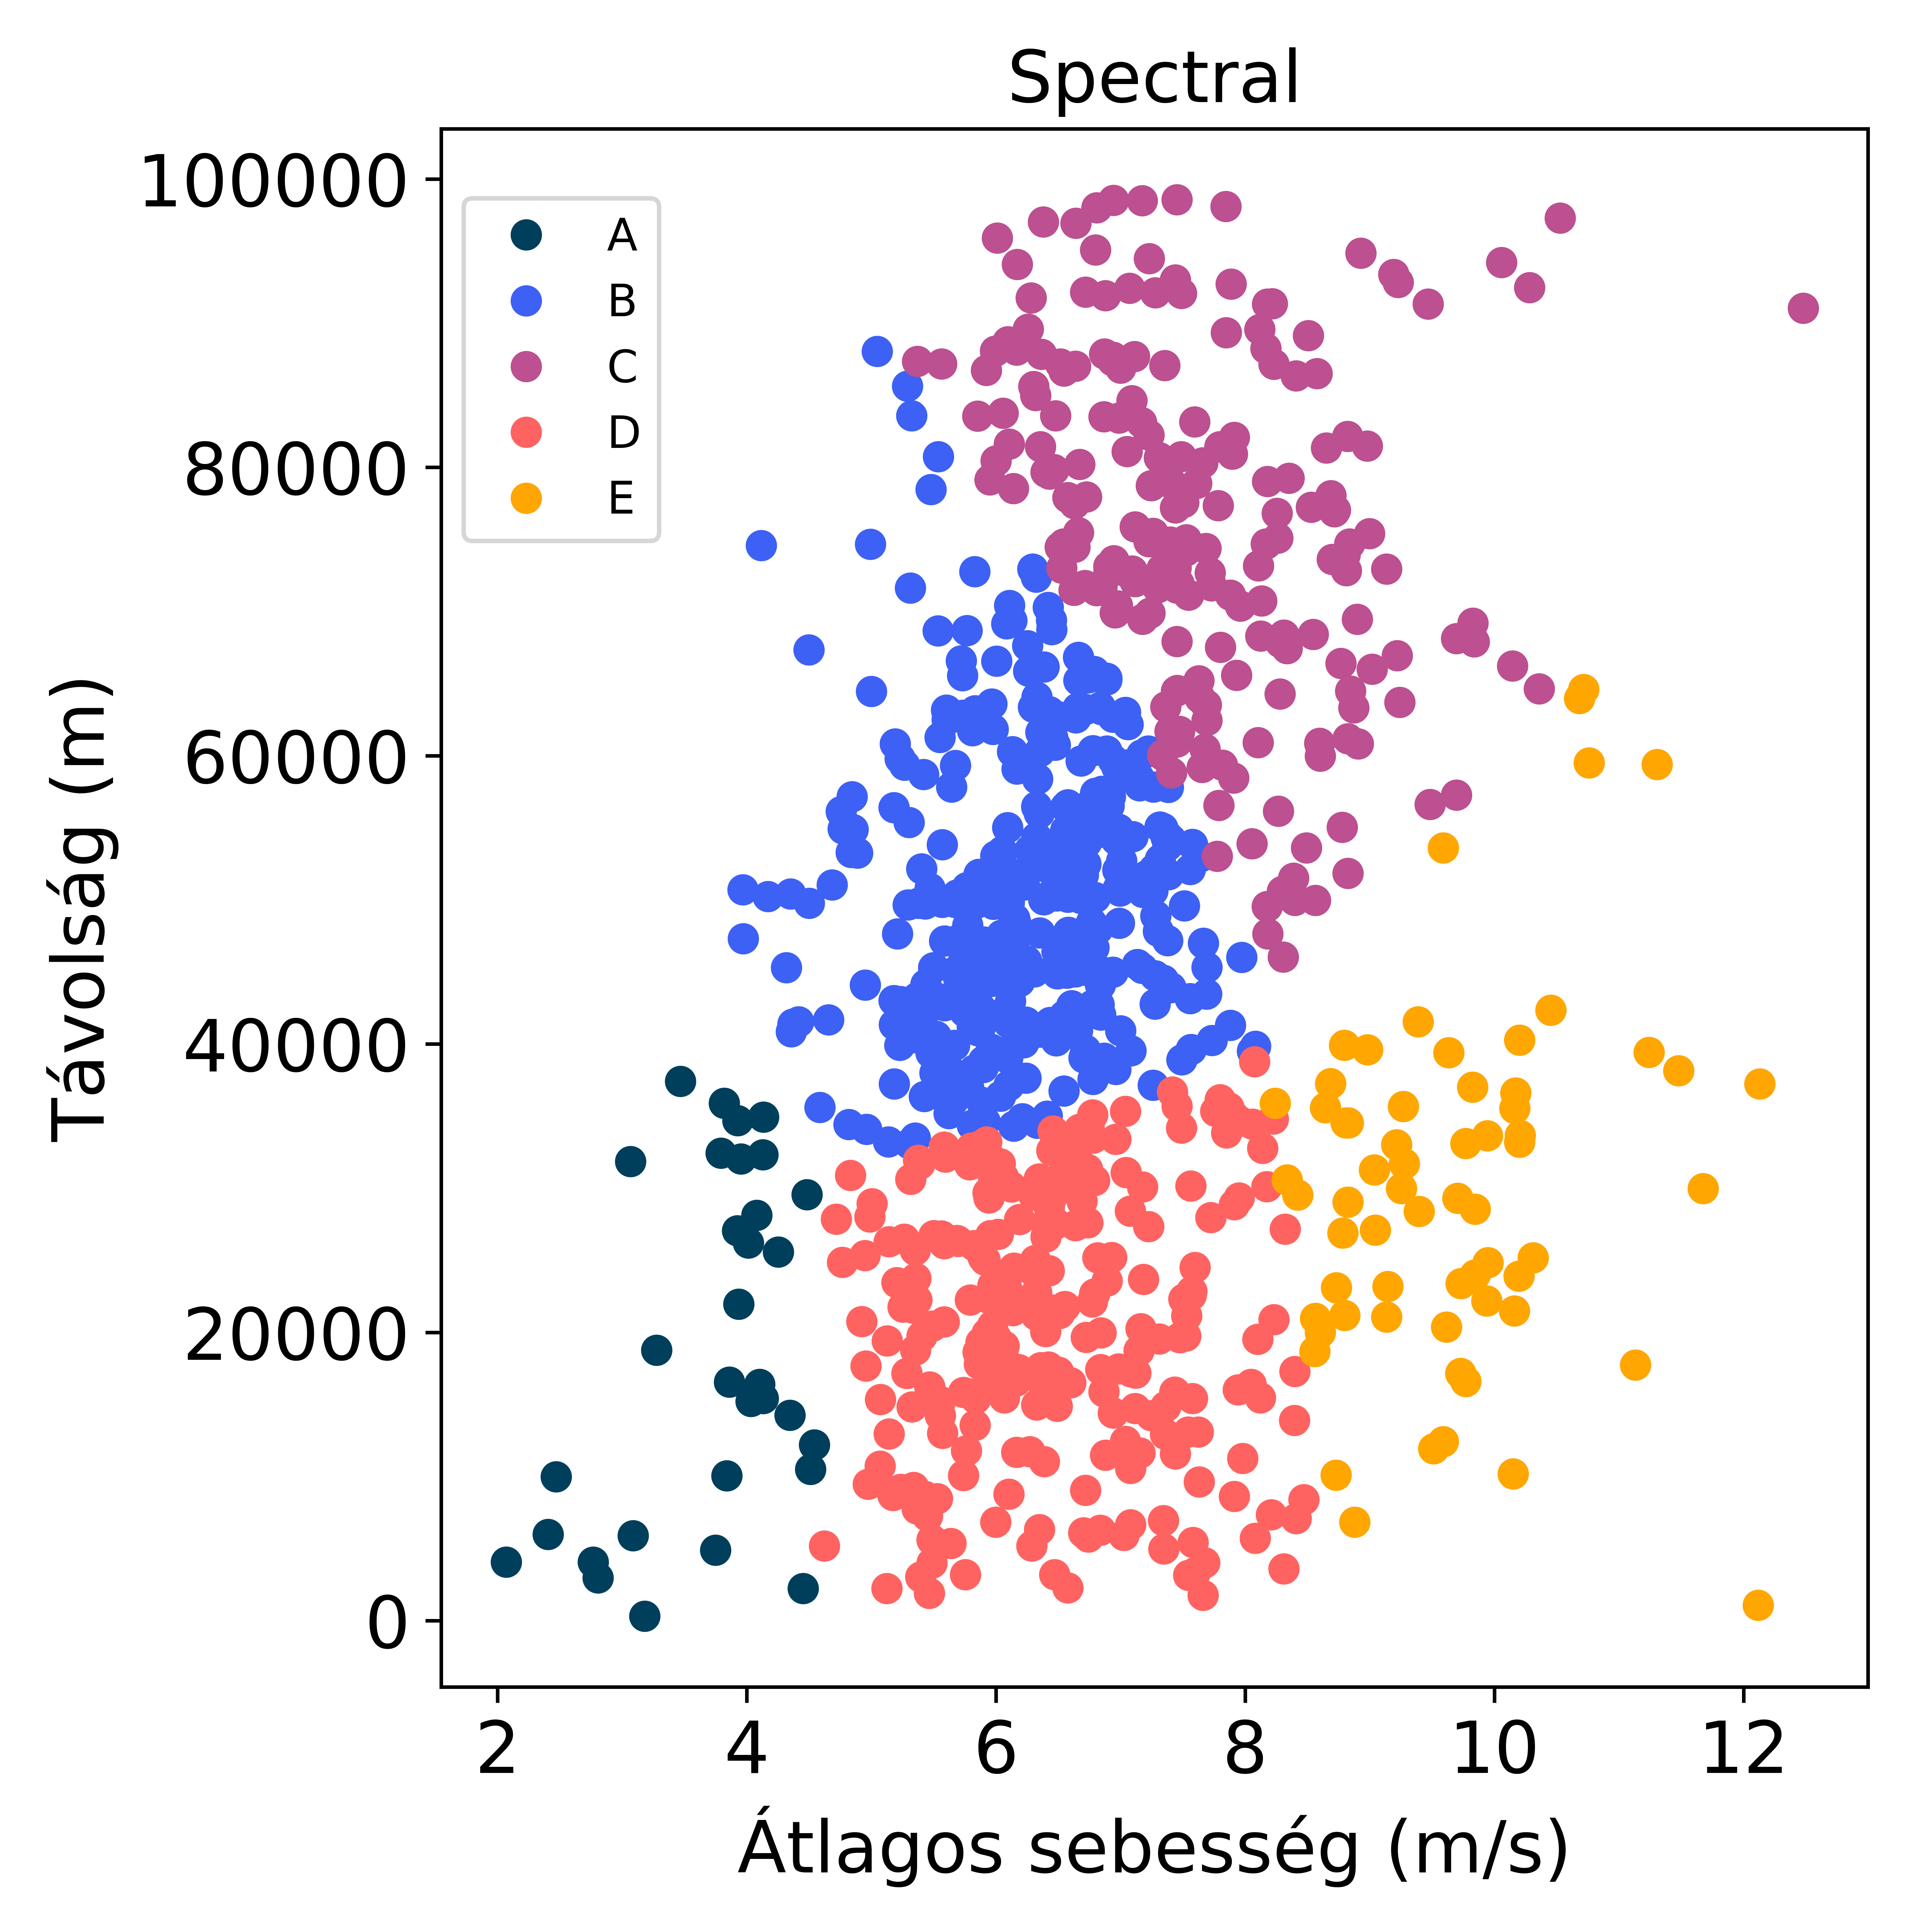
\includegraphics[width=\textwidth,keepaspectratio]{kepek/clustering/age_group_0_spectral_results.png}
		\caption{Spectral}
		\label{subfig:clusteringAgeGroupNullSpectral}
	\end{subfigure}
	\caption{Klaszterezési eredmények a 0. korcsoport adatain}
	\label{fig:clusteringAgeGroupNull}
\end{figure}

A K-Means és a Mini Batch K-Means legnagyobb eltérése az A és B-D klaszterek határán figyelhető meg: a Mini Batch esetén a B-D klaszterek kisebb átlagos sebességű adatokat is tartalmaznak, a klaszter határok közelebb esnek az y tengelyhez. Így az A klaszterbe tartozó adatok mennyisége lényegesen csökken. Továbbá a B és D klaszterek közös határa megközelíti a vízszintest: a K-Means esetén a D klaszterbe tartozó nagy távolságú adatok a Mini Batch módszer esetén átkerülnek a B klaszterbe. A Spectral módszer esetén nagyobbak az eltérések: a B és D klasztereknek lényegesen nagyobb a területük, így az A-ba nagyon kevés útvonal esik. A C és E klaszterek határa lentebb kerül a két K-Means eredményhez képest, a nagy távolságú adatpontok a C klaszterhez fognak tartozni.

Edzés tervezés szempontjából mindhárom klaszter kialakítás felhasználható, megközelítően azonos eredményekkel. A K-Means esetén a klaszter méretek közelebb esnek egymáshoz mint a másik 2 módszerrel, így a javasolt edzést minden klaszter esetén megfelelő mennyiségű adat támasztja alá, azonban a Spectral algoritmus lényegesen jobban körbehatárolható csoportokat alakított ki.

\begin{figure}[!h]
	\centering
	\begin{subfigure}{.5\linewidth}
		\centering
		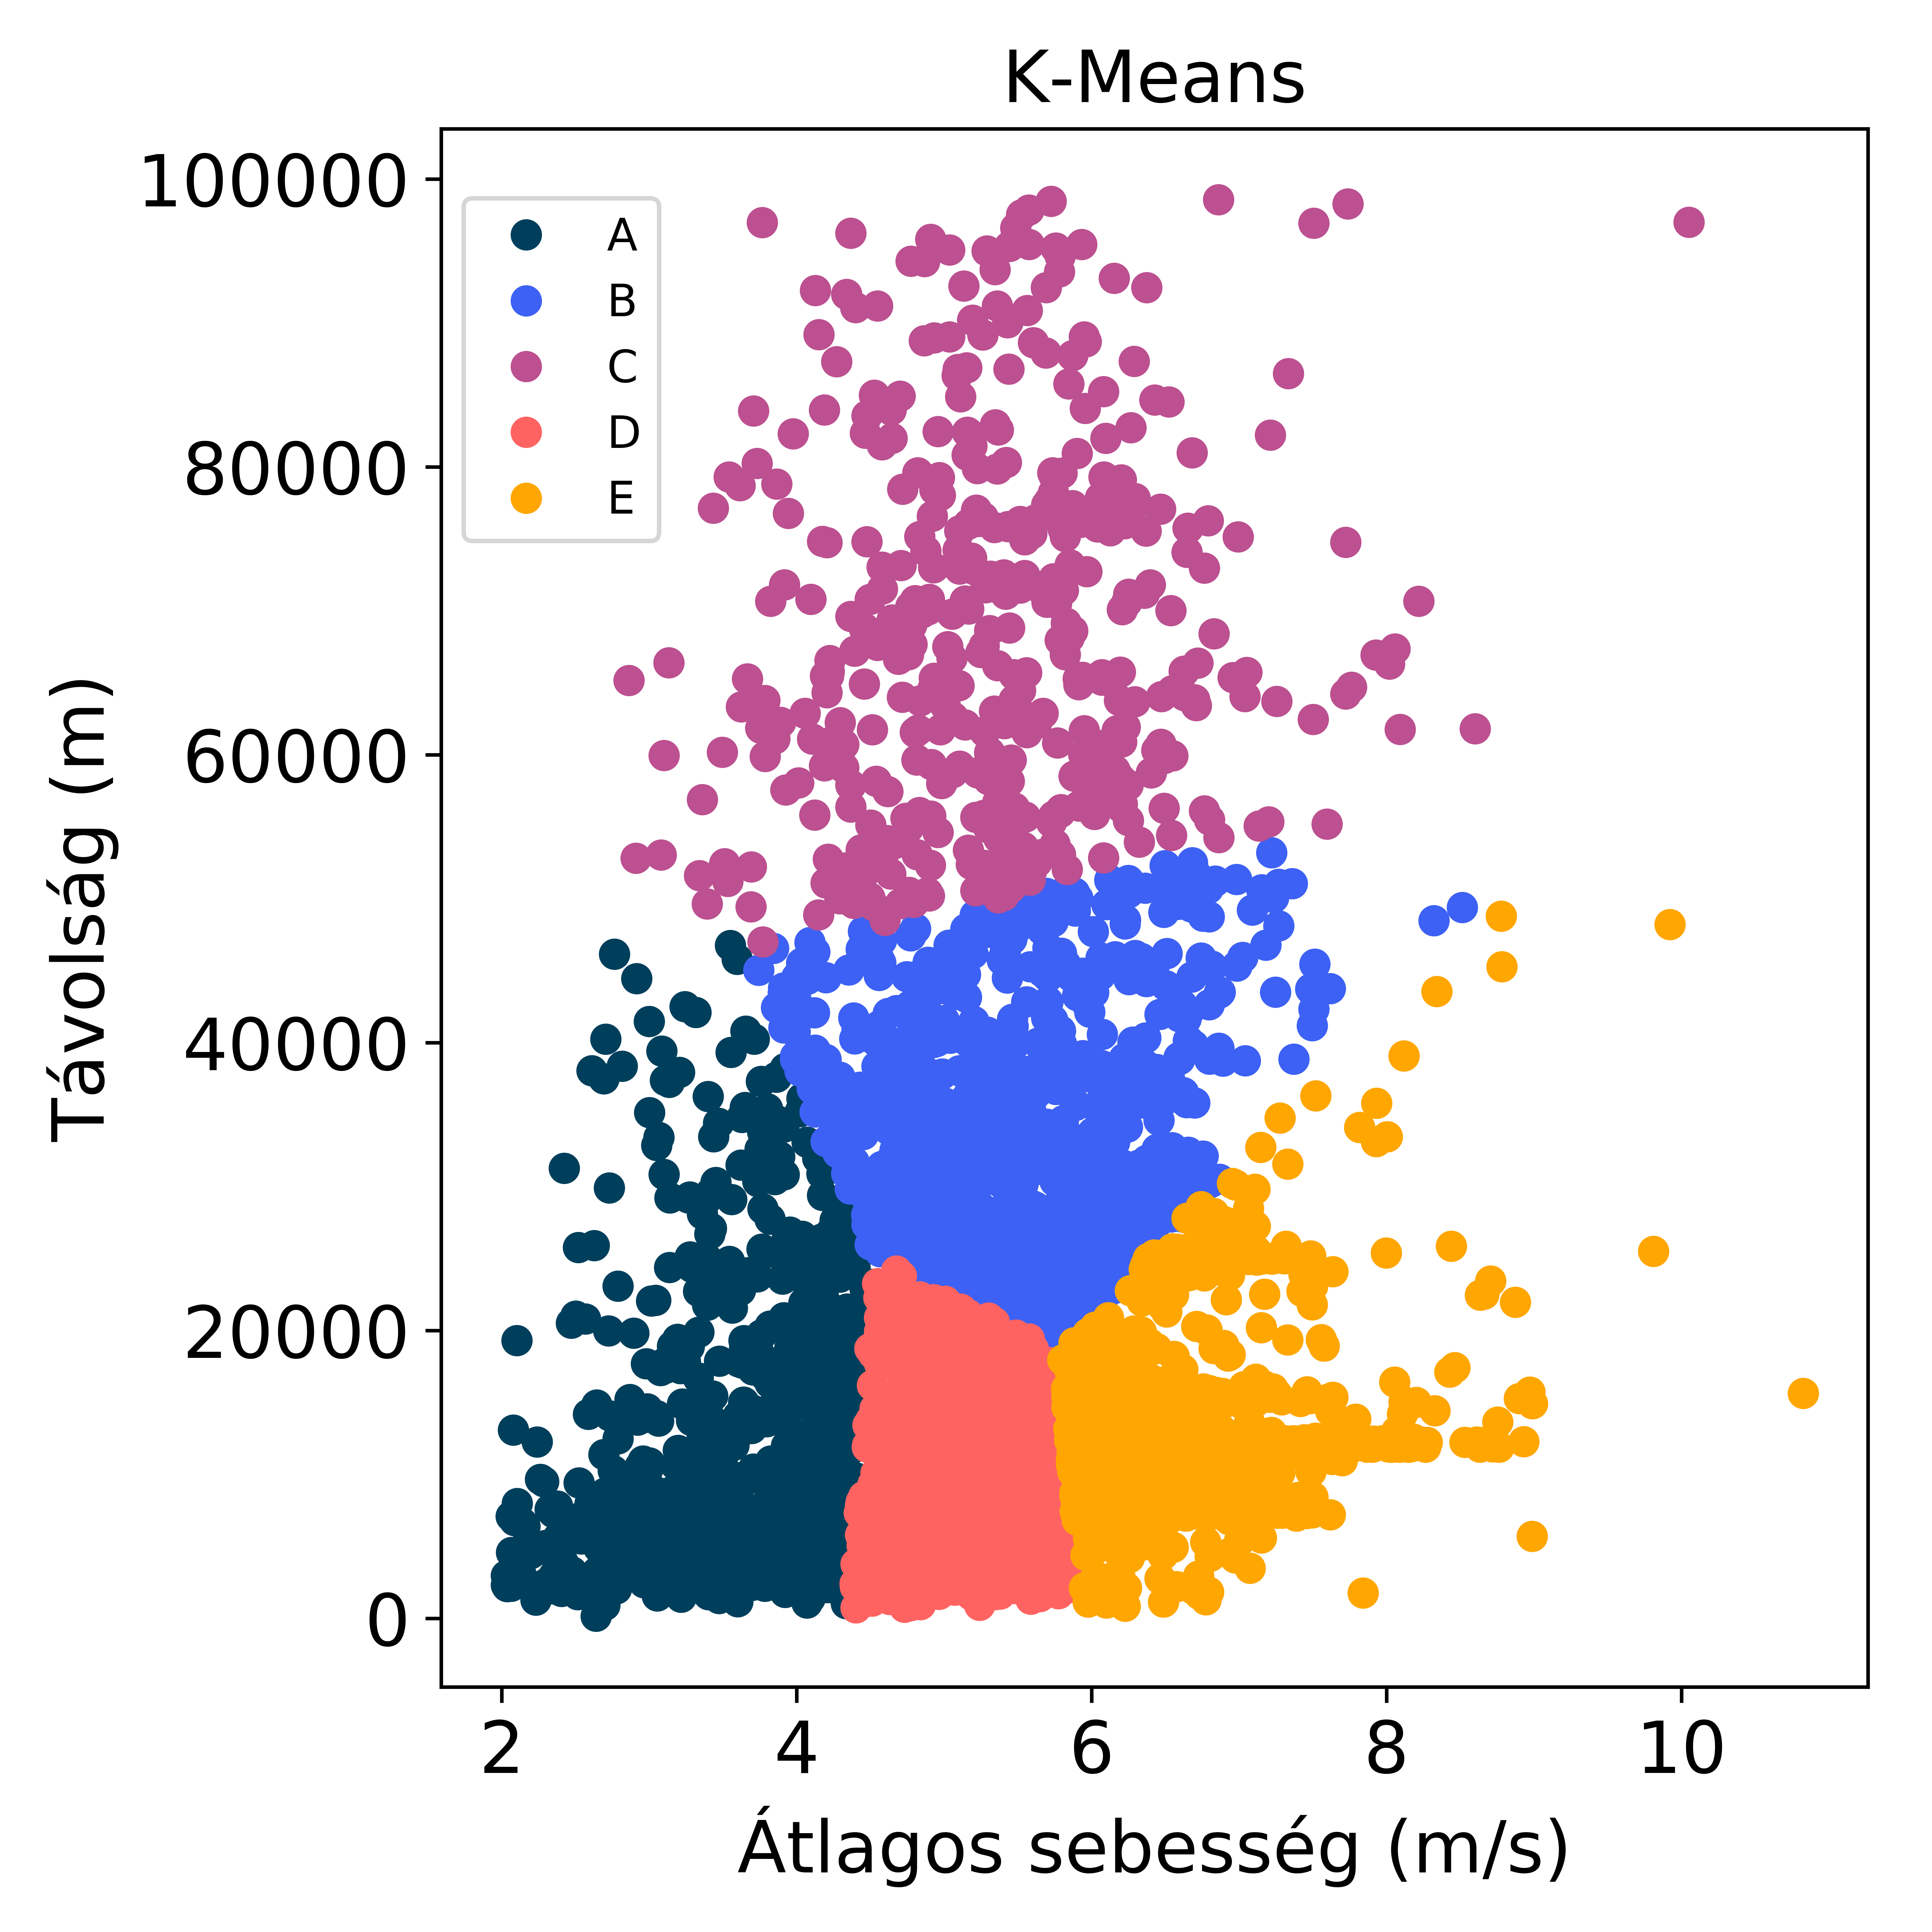
\includegraphics[width=\textwidth,keepaspectratio]{kepek/clustering/age_group_1_kmeans_results.png}
		\caption{K-Means}
		\label{subfig:clusteringAgeGroupOneKmeans}
	\end{subfigure}%
	\begin{subfigure}{.5\linewidth}
		\centering
		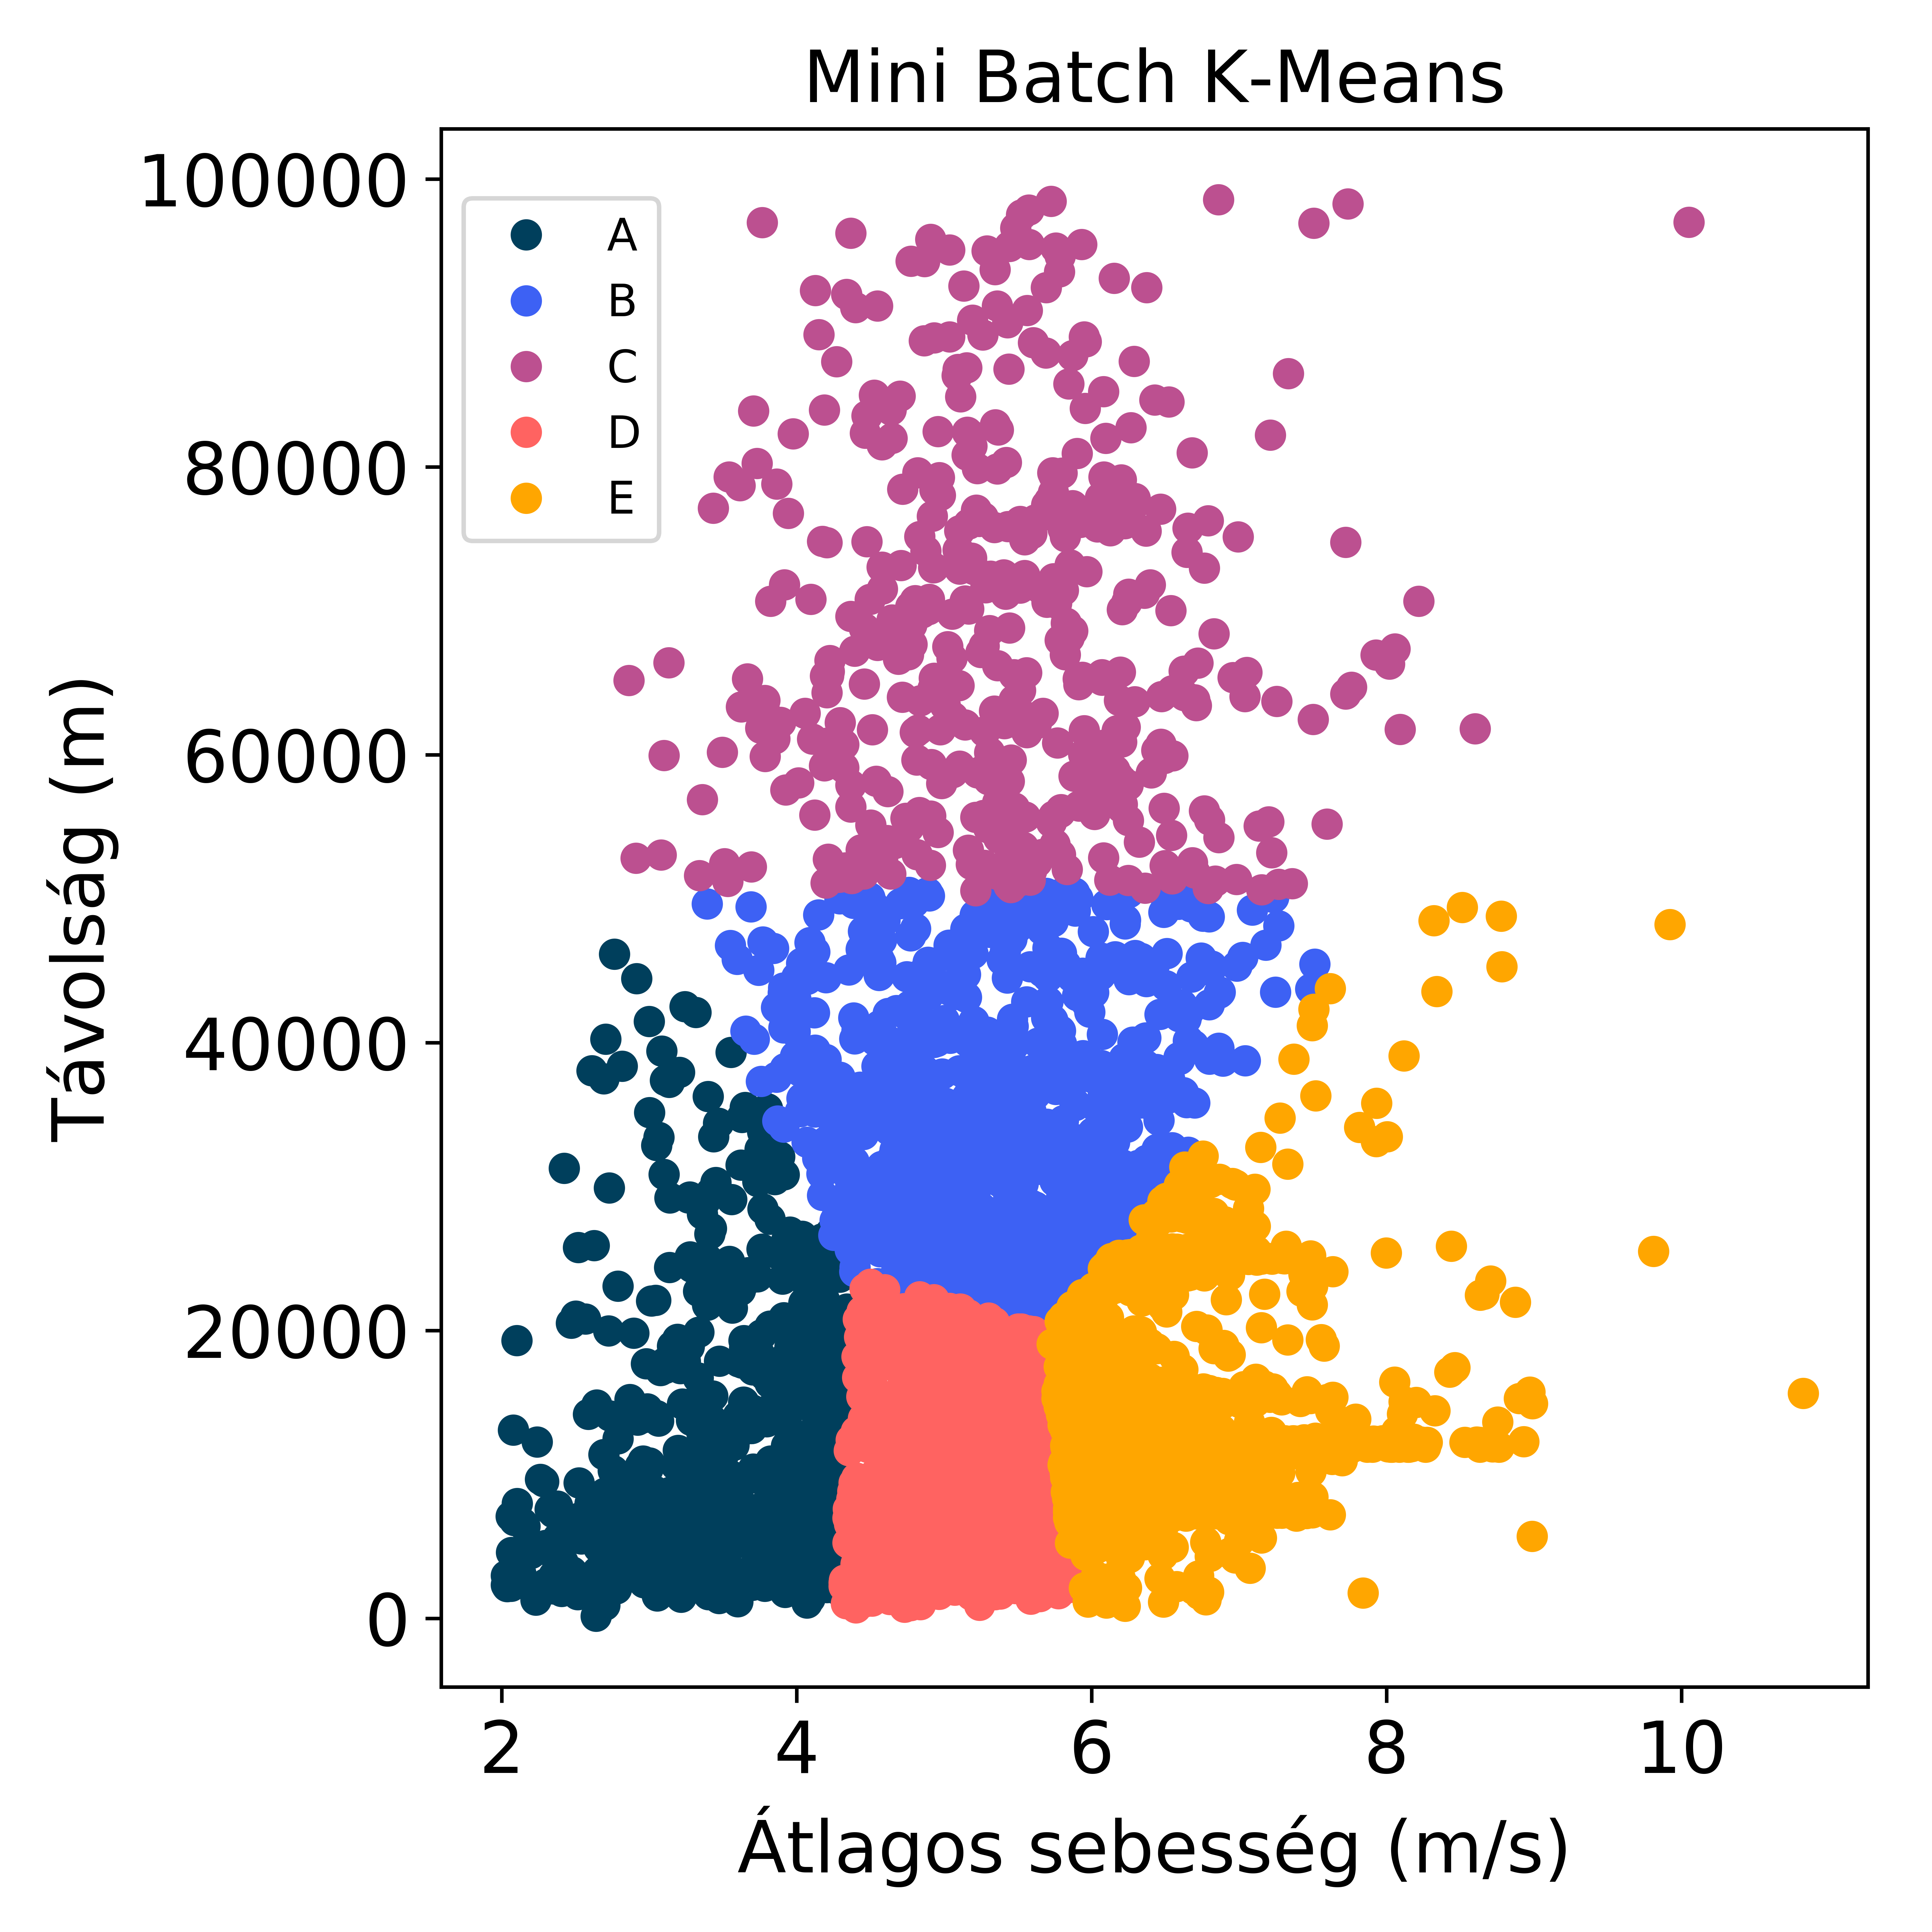
\includegraphics[width=\textwidth,keepaspectratio]{kepek/clustering/age_group_1_minibatch_results.png}
		\caption{Mini Batch K-Means}
		\label{subfig:clusteringAgeGroupOneMiniBatch}
	\end{subfigure}\\[1ex]
	\begin{subfigure}{.5\linewidth}
		\centering
		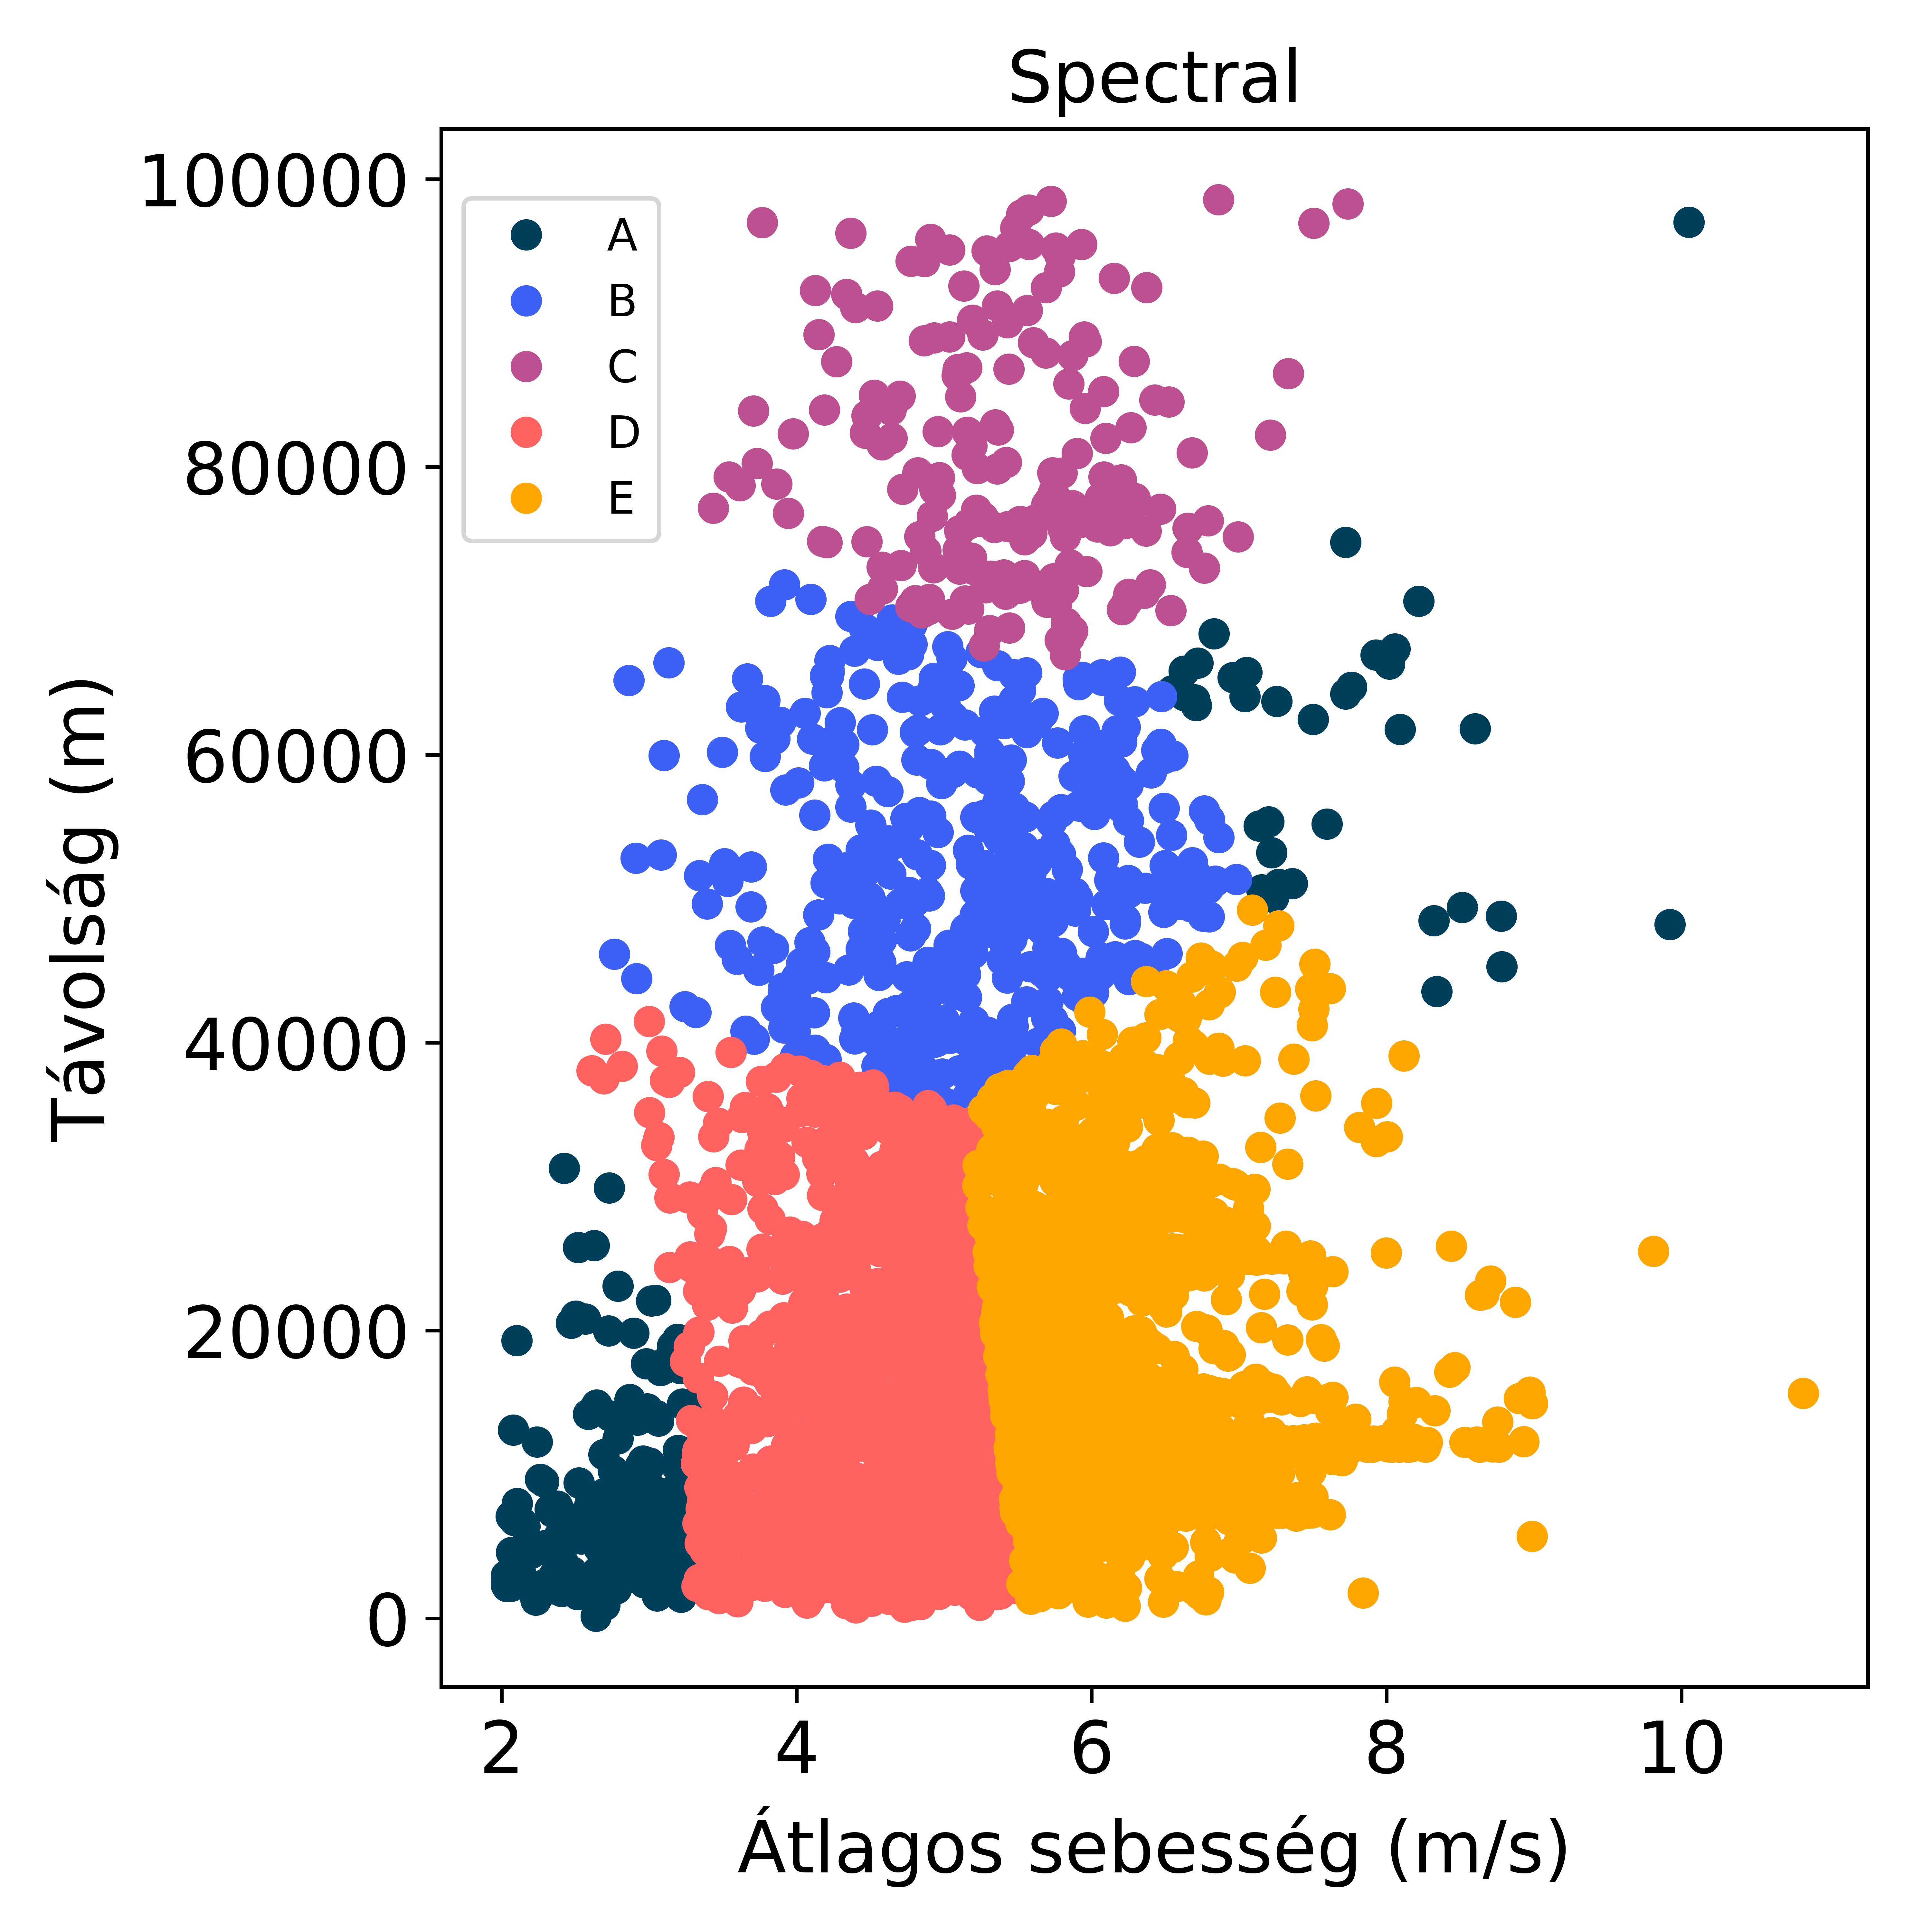
\includegraphics[width=\textwidth,keepaspectratio]{kepek/clustering/age_group_1_spectral_results.png}
		\caption{Spectral}
		\label{subfig:clusteringAgeGroupOneSpectral}
	\end{subfigure}
	\caption{Klaszterezési eredmények a 1. korcsoport adatain}
	\label{fig:clusteringAgeGroupOne}
\end{figure}

\SubSection{1. korcsoport}

A részhalmaz összesen 7219 útvonalat tartalmaz. A különböző klaszterezési eljárások eredményei a \myref{fig:clusteringAgeGroupOne} ábrán láthatóak. A kialakított klaszterek elhelyezkedése a két K-Means esetén nagy vonalakban megegyezik, ezeket általánosan az alábbi módon lehetne jellemezni:
%\noindent \textbf{Klaszterek jellemzése:}
\begin{itemize}
	\item A : normális és nagy távolság - normális és extra magas átlagsebesség
	\item B : nagy távolság - normális átlagsebesség
	\item C : extrém nagy távolság - magas és extrém magas átlagsebesség
	\item D : normális távolság - magas átlagsebesség
	\item E : normális és nagy távolság - extrém magas átlagsebesség
\end{itemize}
Ezzel szemben a \myref{subfig:clusteringAgeGroupOneSpectral} ábrán látható Spectral klaszterezési eredmények nagy mértékben különbözőek, érdekes módon az A klaszter két részre szakad. Ez annak az eredménye lehet hogy a Spectral eljárás a klaszterek kialakítása során dimenzió redukálást végez, és a csökkentett dimenziószám alapján keresi az kapcsolódó adatpontokat. Ez az eredmény edzés tervezéshez nem kifejezetten használható, a kialakult klasztereket nem lehet könnyen körbehatárolni.



\SubSection{2. korcsoport}

\begin{figure}[!h]
	\centering
	\begin{subfigure}{.5\linewidth}
		\centering
		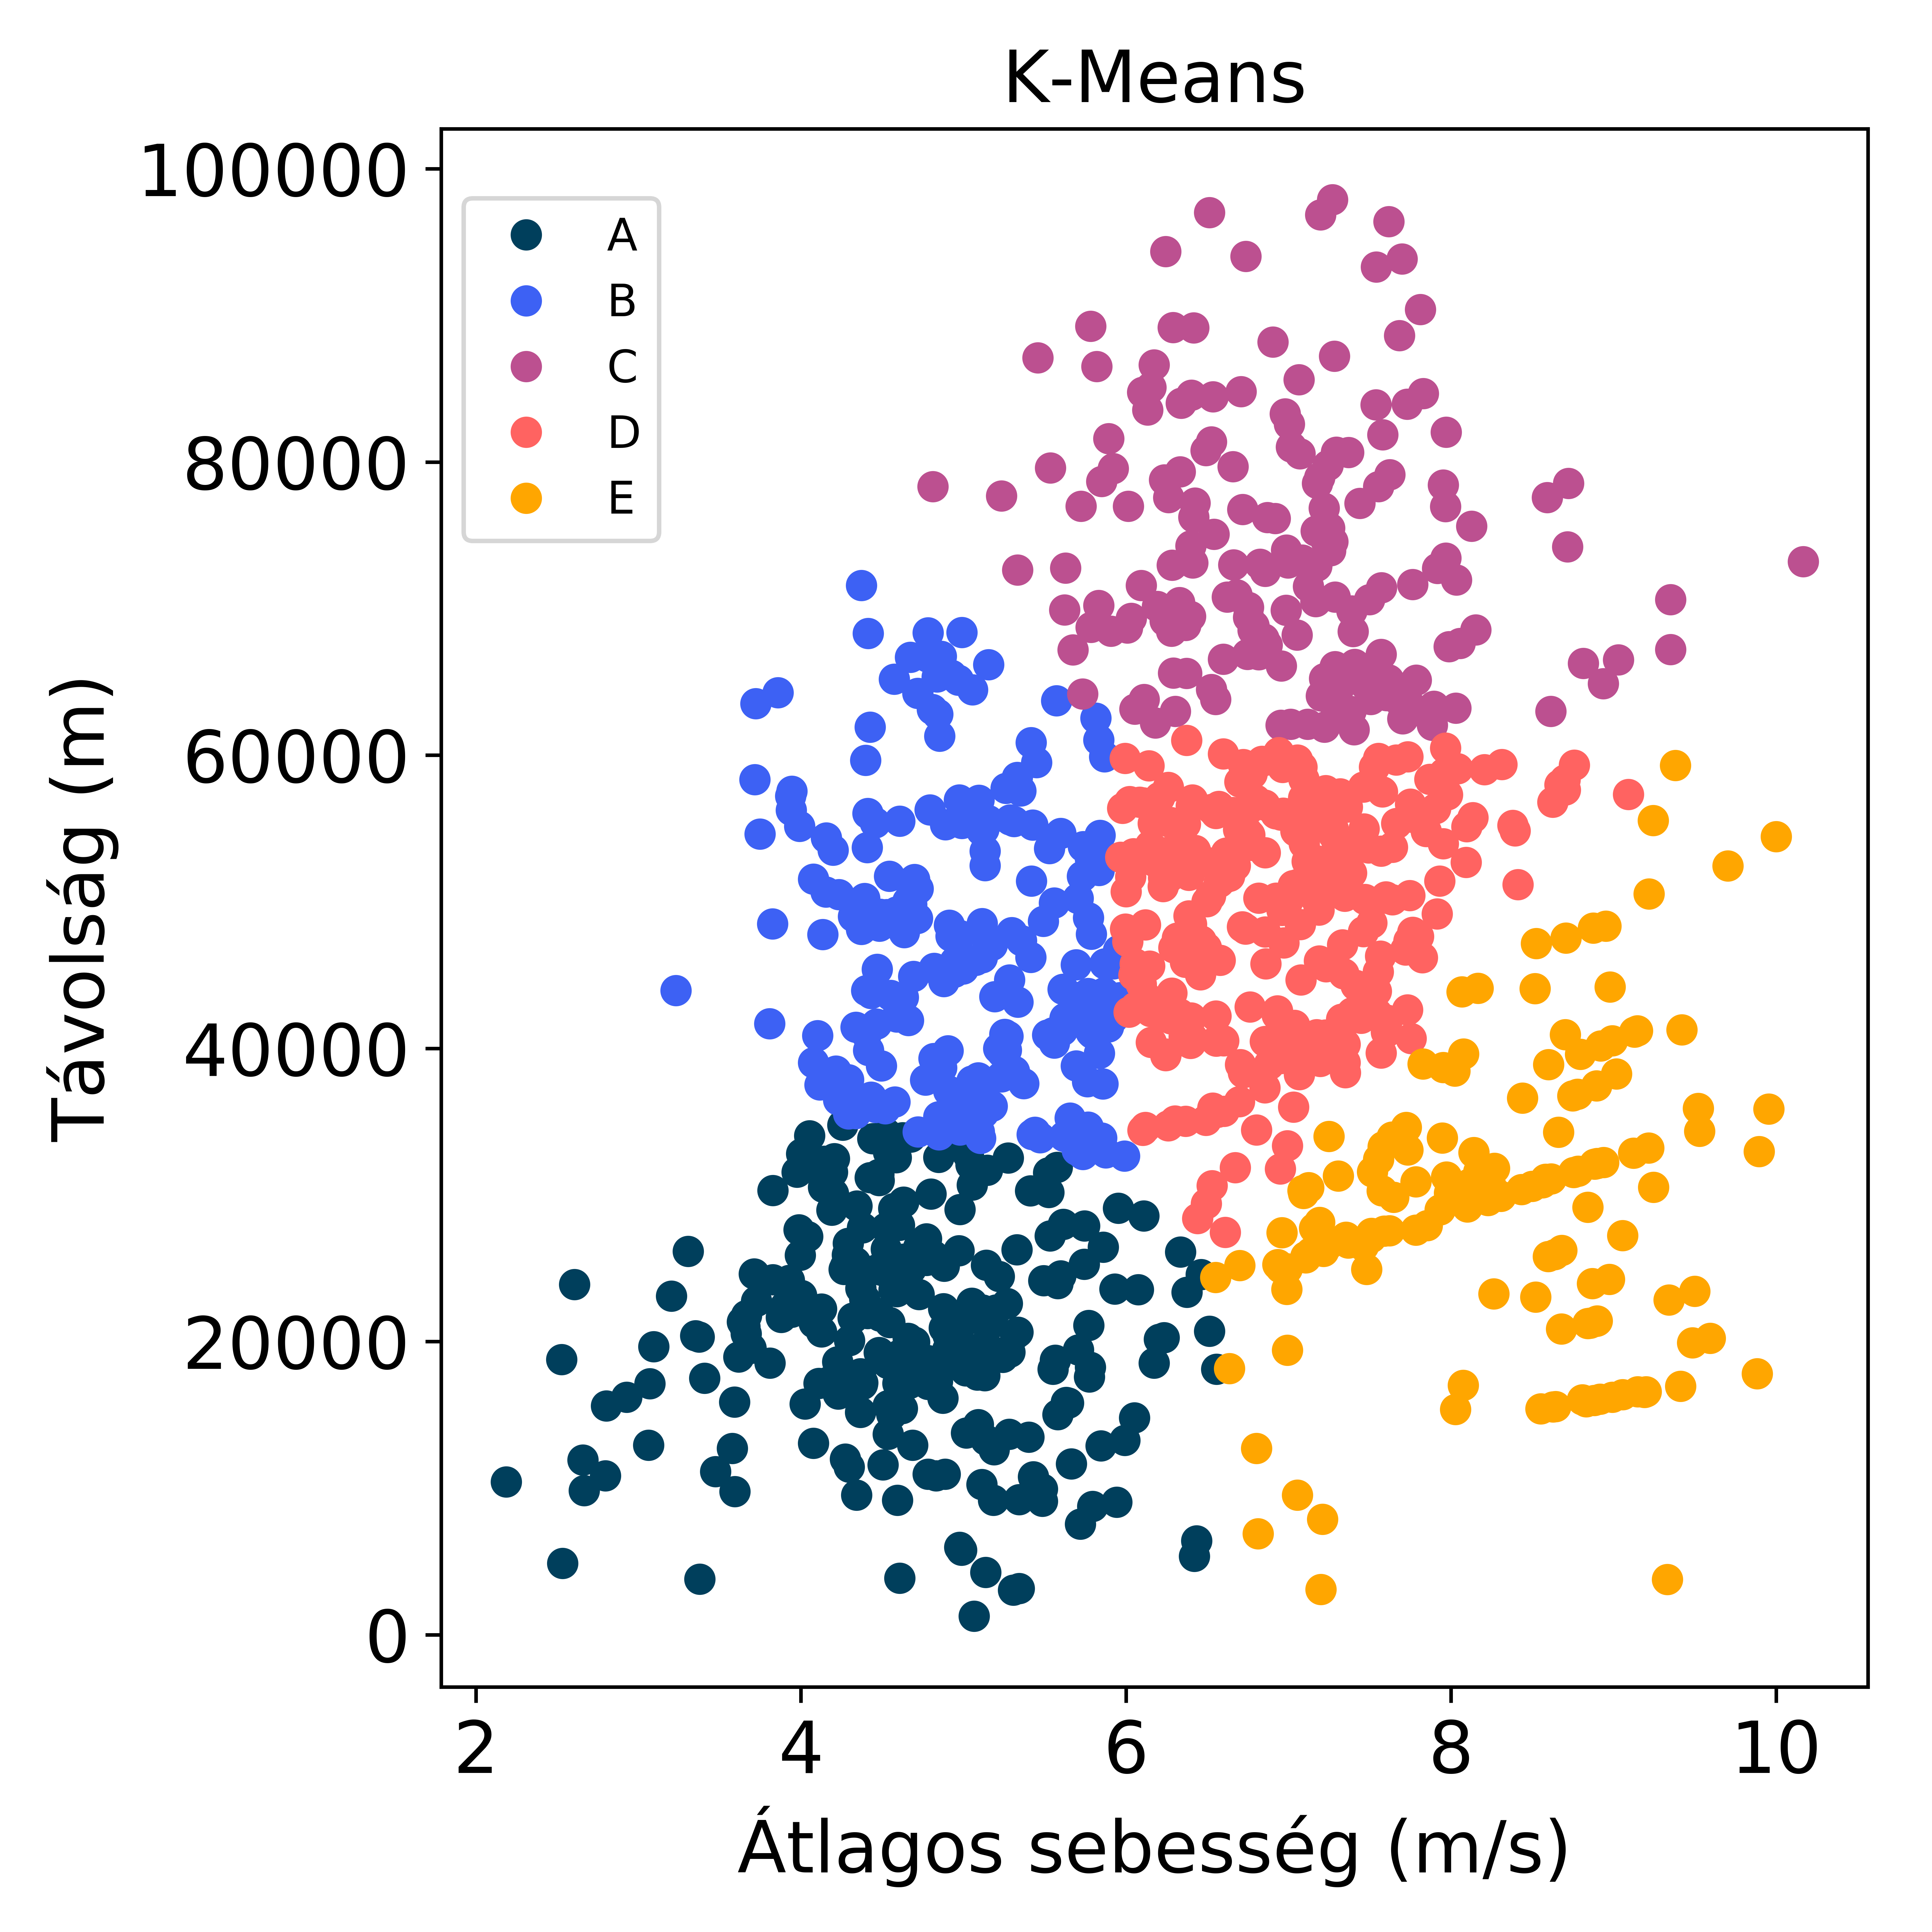
\includegraphics[width=\textwidth,keepaspectratio]{kepek/clustering/age_group_2_kmeans_results.png}
		\caption{K-Means}
		\label{subfig:clusteringAgeGroupTwoKmeans}
	\end{subfigure}%
	\begin{subfigure}{.5\linewidth}
		\centering
		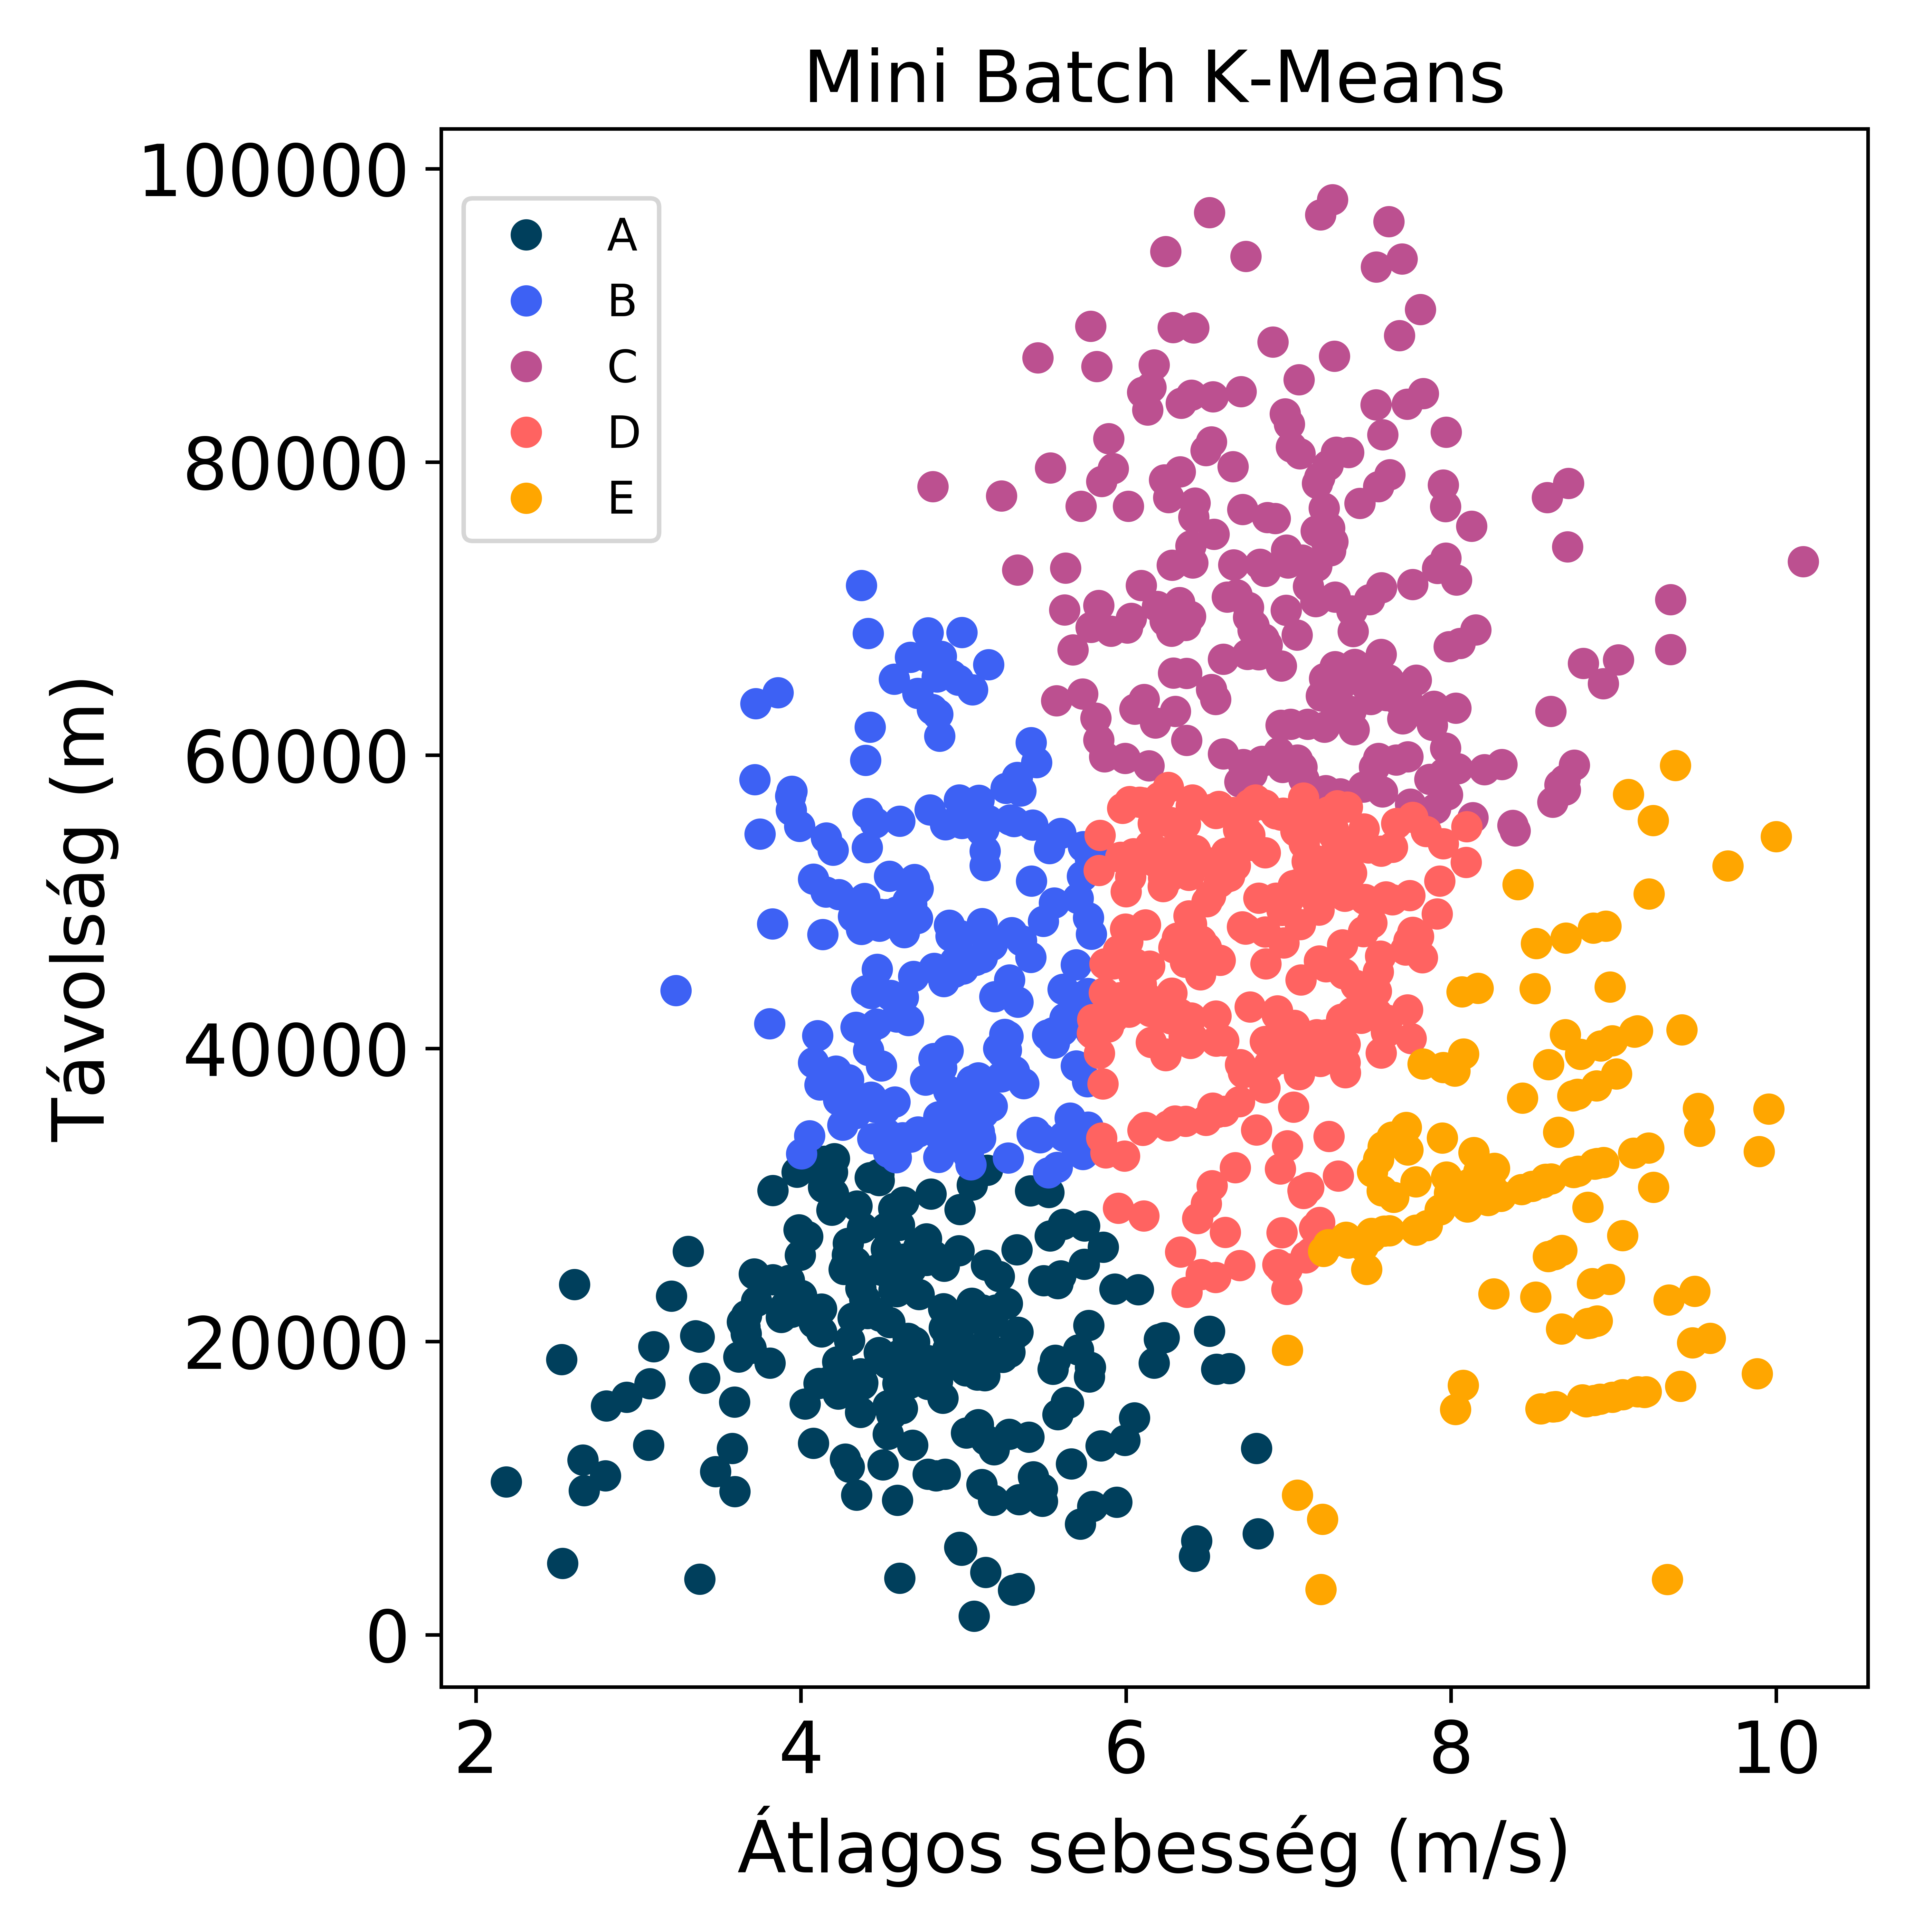
\includegraphics[width=\textwidth,keepaspectratio]{kepek/clustering/age_group_2_minibatch_results.png}
		\caption{Mini Batch K-Means}
		\label{subfig:clusteringAgeGroupTwoMiniBatch}
	\end{subfigure}\\[1ex]
	\begin{subfigure}{.5\linewidth}
		\centering
		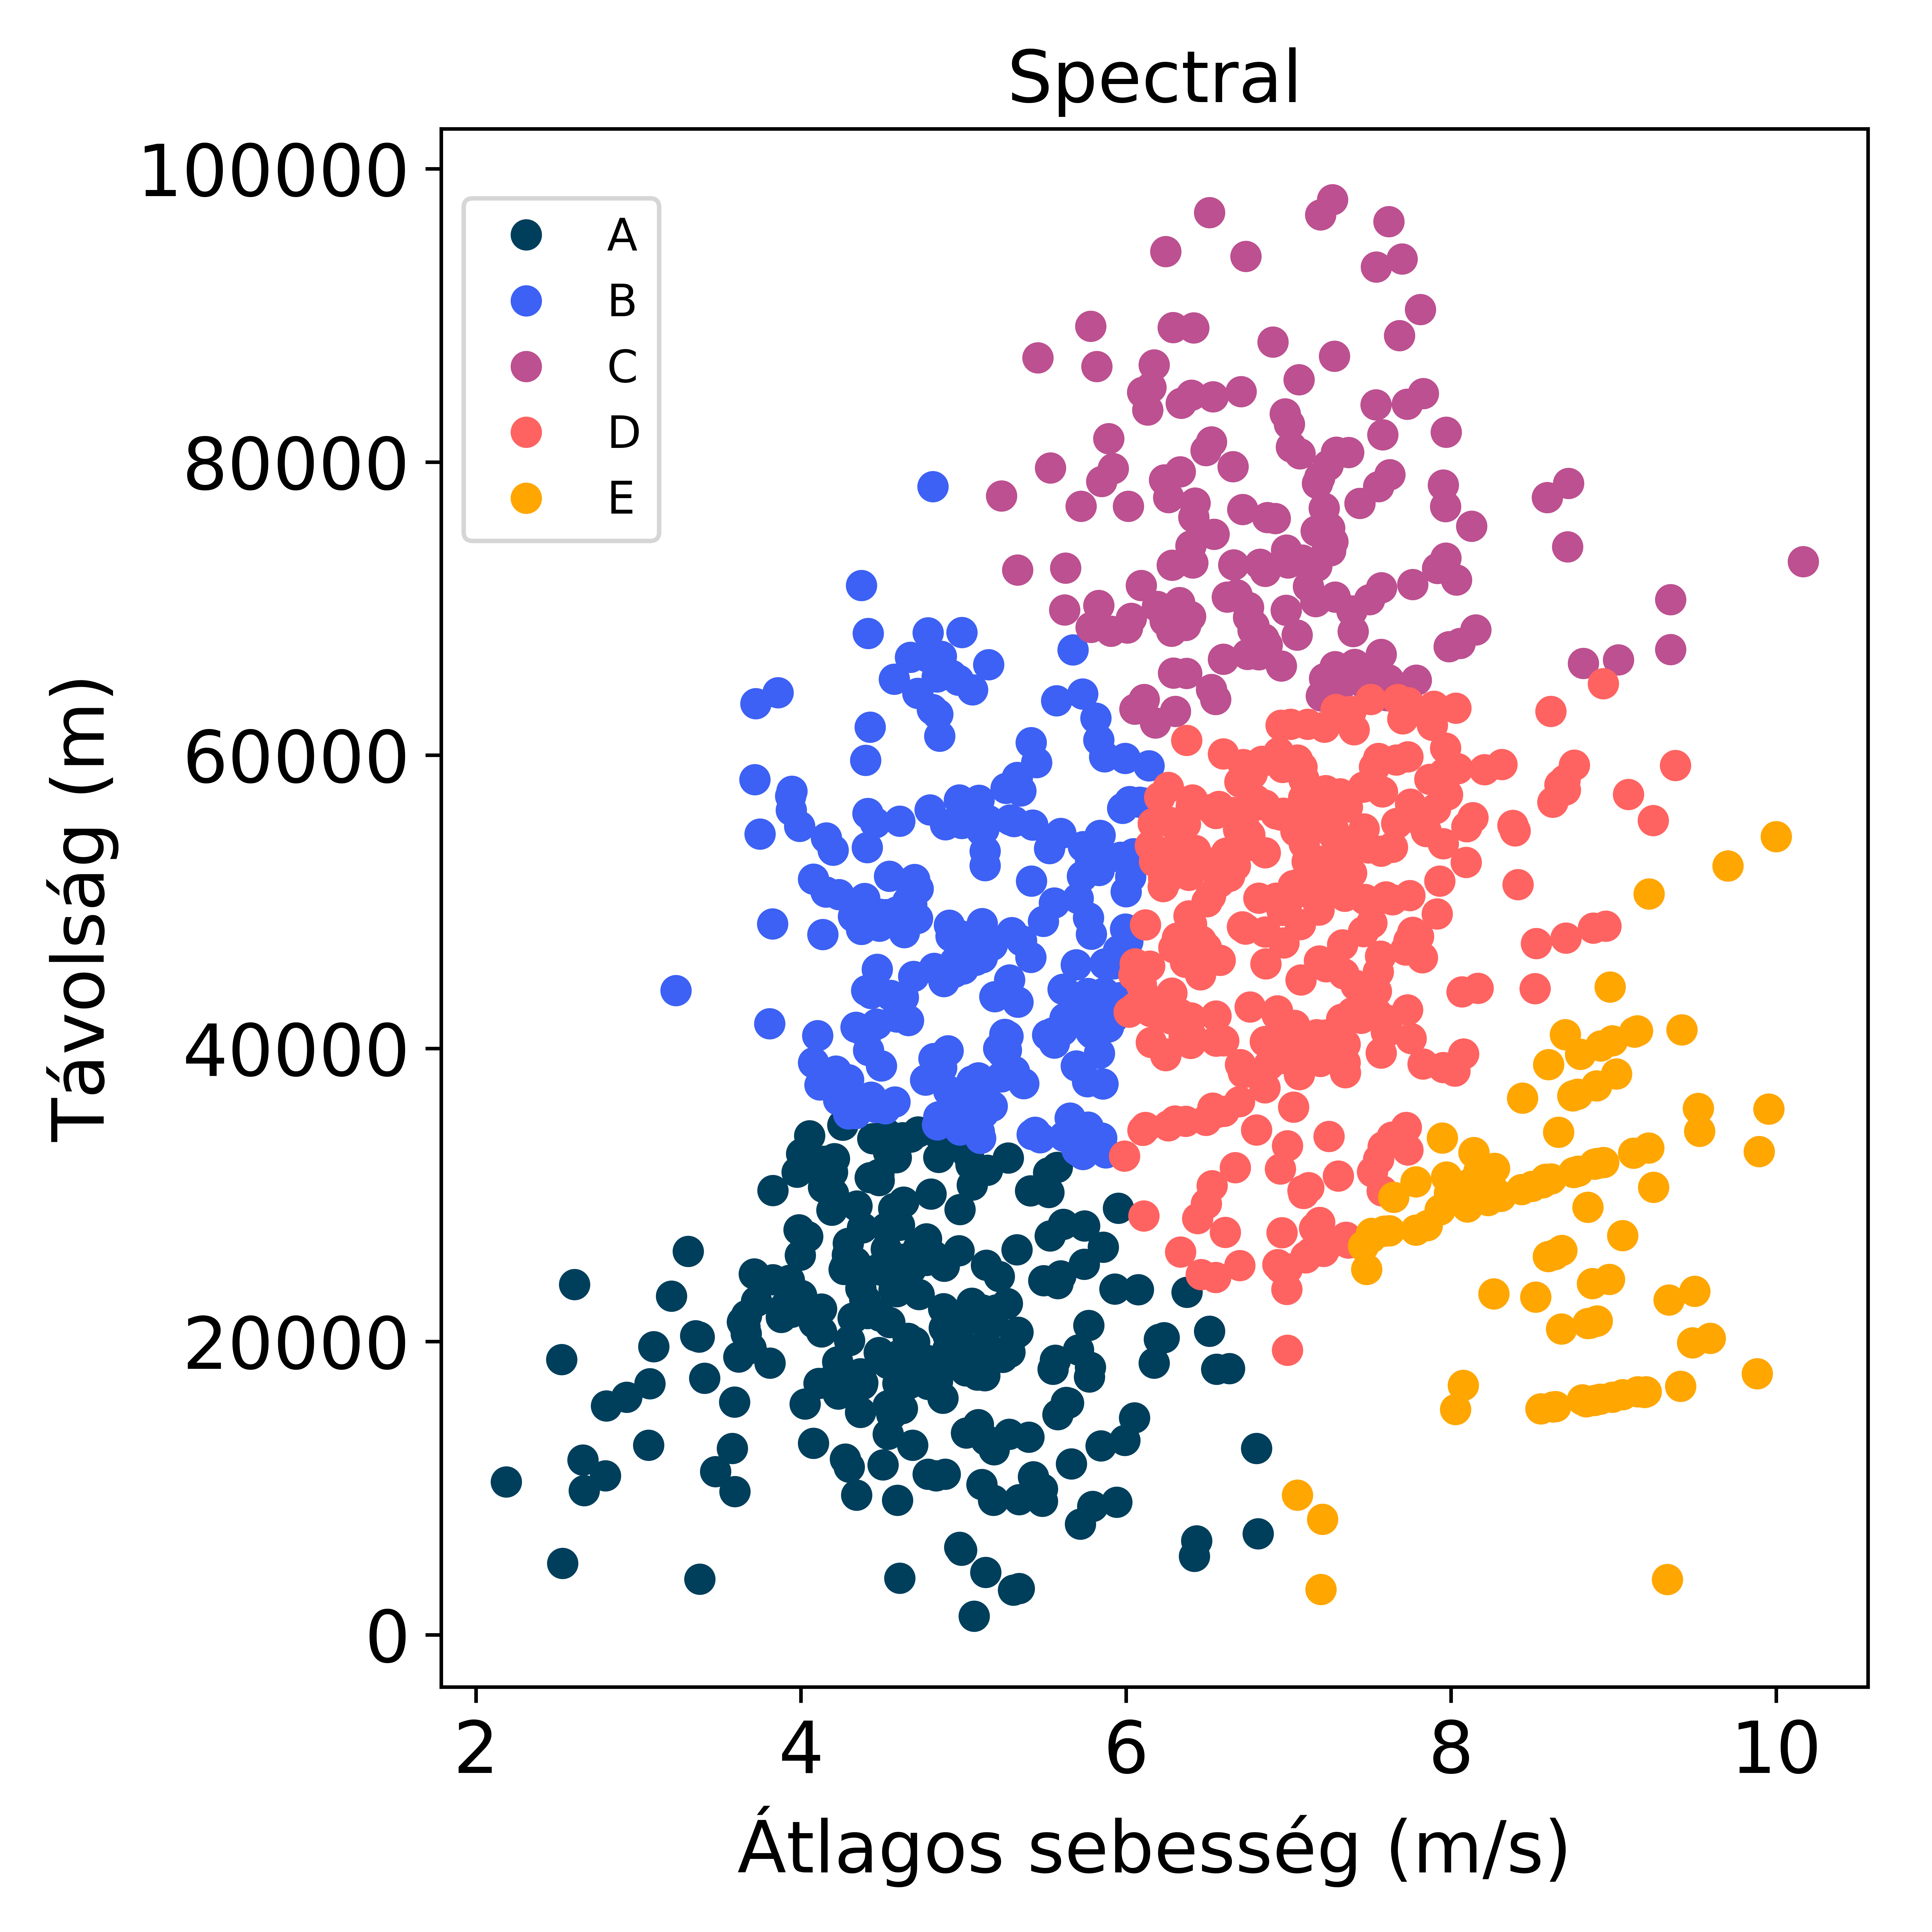
\includegraphics[width=\textwidth,keepaspectratio]{kepek/clustering/age_group_2_spectral_results.png}
		\caption{Spectral}
		\label{subfig:clusteringAgeGroupTwoSpectral}
	\end{subfigure}
	\caption{Klaszterezési eredmények a 2. korcsoport adatain}
	\label{fig:clusteringAgeGroupTwo}
\end{figure}

A részhalmaz összesen 1050 útvonalat tartalmaz. A különböző klaszterezési eljárások eredményei a \myref{fig:clusteringAgeGroupTwo} ábrán láthatóak. A kialakított klaszterek kis mértékben térnek el egymástól, a következő képen lehet jellemezni őket:
\begin{itemize}
	\item A : normális távolság - normális átlagsebesség
	\item B : nagy távolság - normális átlagsebesség
	\item C : extrém nagy távolság - magas és extrém magas átlagsebesség
	\item D : nagy távolság - magas átlagsebesség
	\item E : normális távolság -  extrém magas átlagsebesség
\end{itemize}

A K-Means és a Mini Batch módszerek eltérése főleg a D klaszter esetében figyelhető meg: a K-Means eredményeihez képest a felső határ lentebb hajlik, a nagy távolságú és magas sebességű pontok átkerülnek a C klaszterbe, valamint ezzel egyidejűleg az E klaszterből néhány kis távolságú pont a D klaszterbe kerül.

A K-Means variációk és a Spectral klaszterezés különbsége ezen az adathalmazon szintén a D klaszter kiemelésével figyelhető meg a legegyszerűbben. A D klaszter gyakorlatilag minden irányba kitágul, a szomszédos csoportok határoló pontjai átkerülnek hozzá, ez alól kivételt csak a B C D klaszterek találkozása képez.

Az eredményül kapott klaszterek mindegyike felhasználható edzés javaslat készítésére, természetesen kicsit eltérő eredményekkel.

\SubSection{Összefoglalás}
A három korcsoport alapján készült klaszterek eltérései jól láthatóak a \myref{fig:clusteringAgeGroupNull}, \myref{fig:clusteringAgeGroupOne}, és a \myref{fig:clusteringAgeGroupTwo} ábrán. Felhasználásukkal minden korcsoportra egyedi edzés javaslat készíthető, figyelembe véve hogy a felhasználó az egyes klaszterek jellemzése alapján milyen jellegű és nehézségű edzést szeretne végezni. Az edzés javaslatok készítésére a \myref{prog:getTrainingSuggestion} program részlet szolgál, ennek néhány eredménye az alábbiakban látható. Mind a három korcsoportra 3 edzés javaslat készült az C, D és E típusú klaszterek alapján, minden esetben C - normál, D - könnyű és E - nehéz fokozattal.

\begin{figure}[!h]
	\centering
	\begin{subfigure}{.5\linewidth}
		\centering
		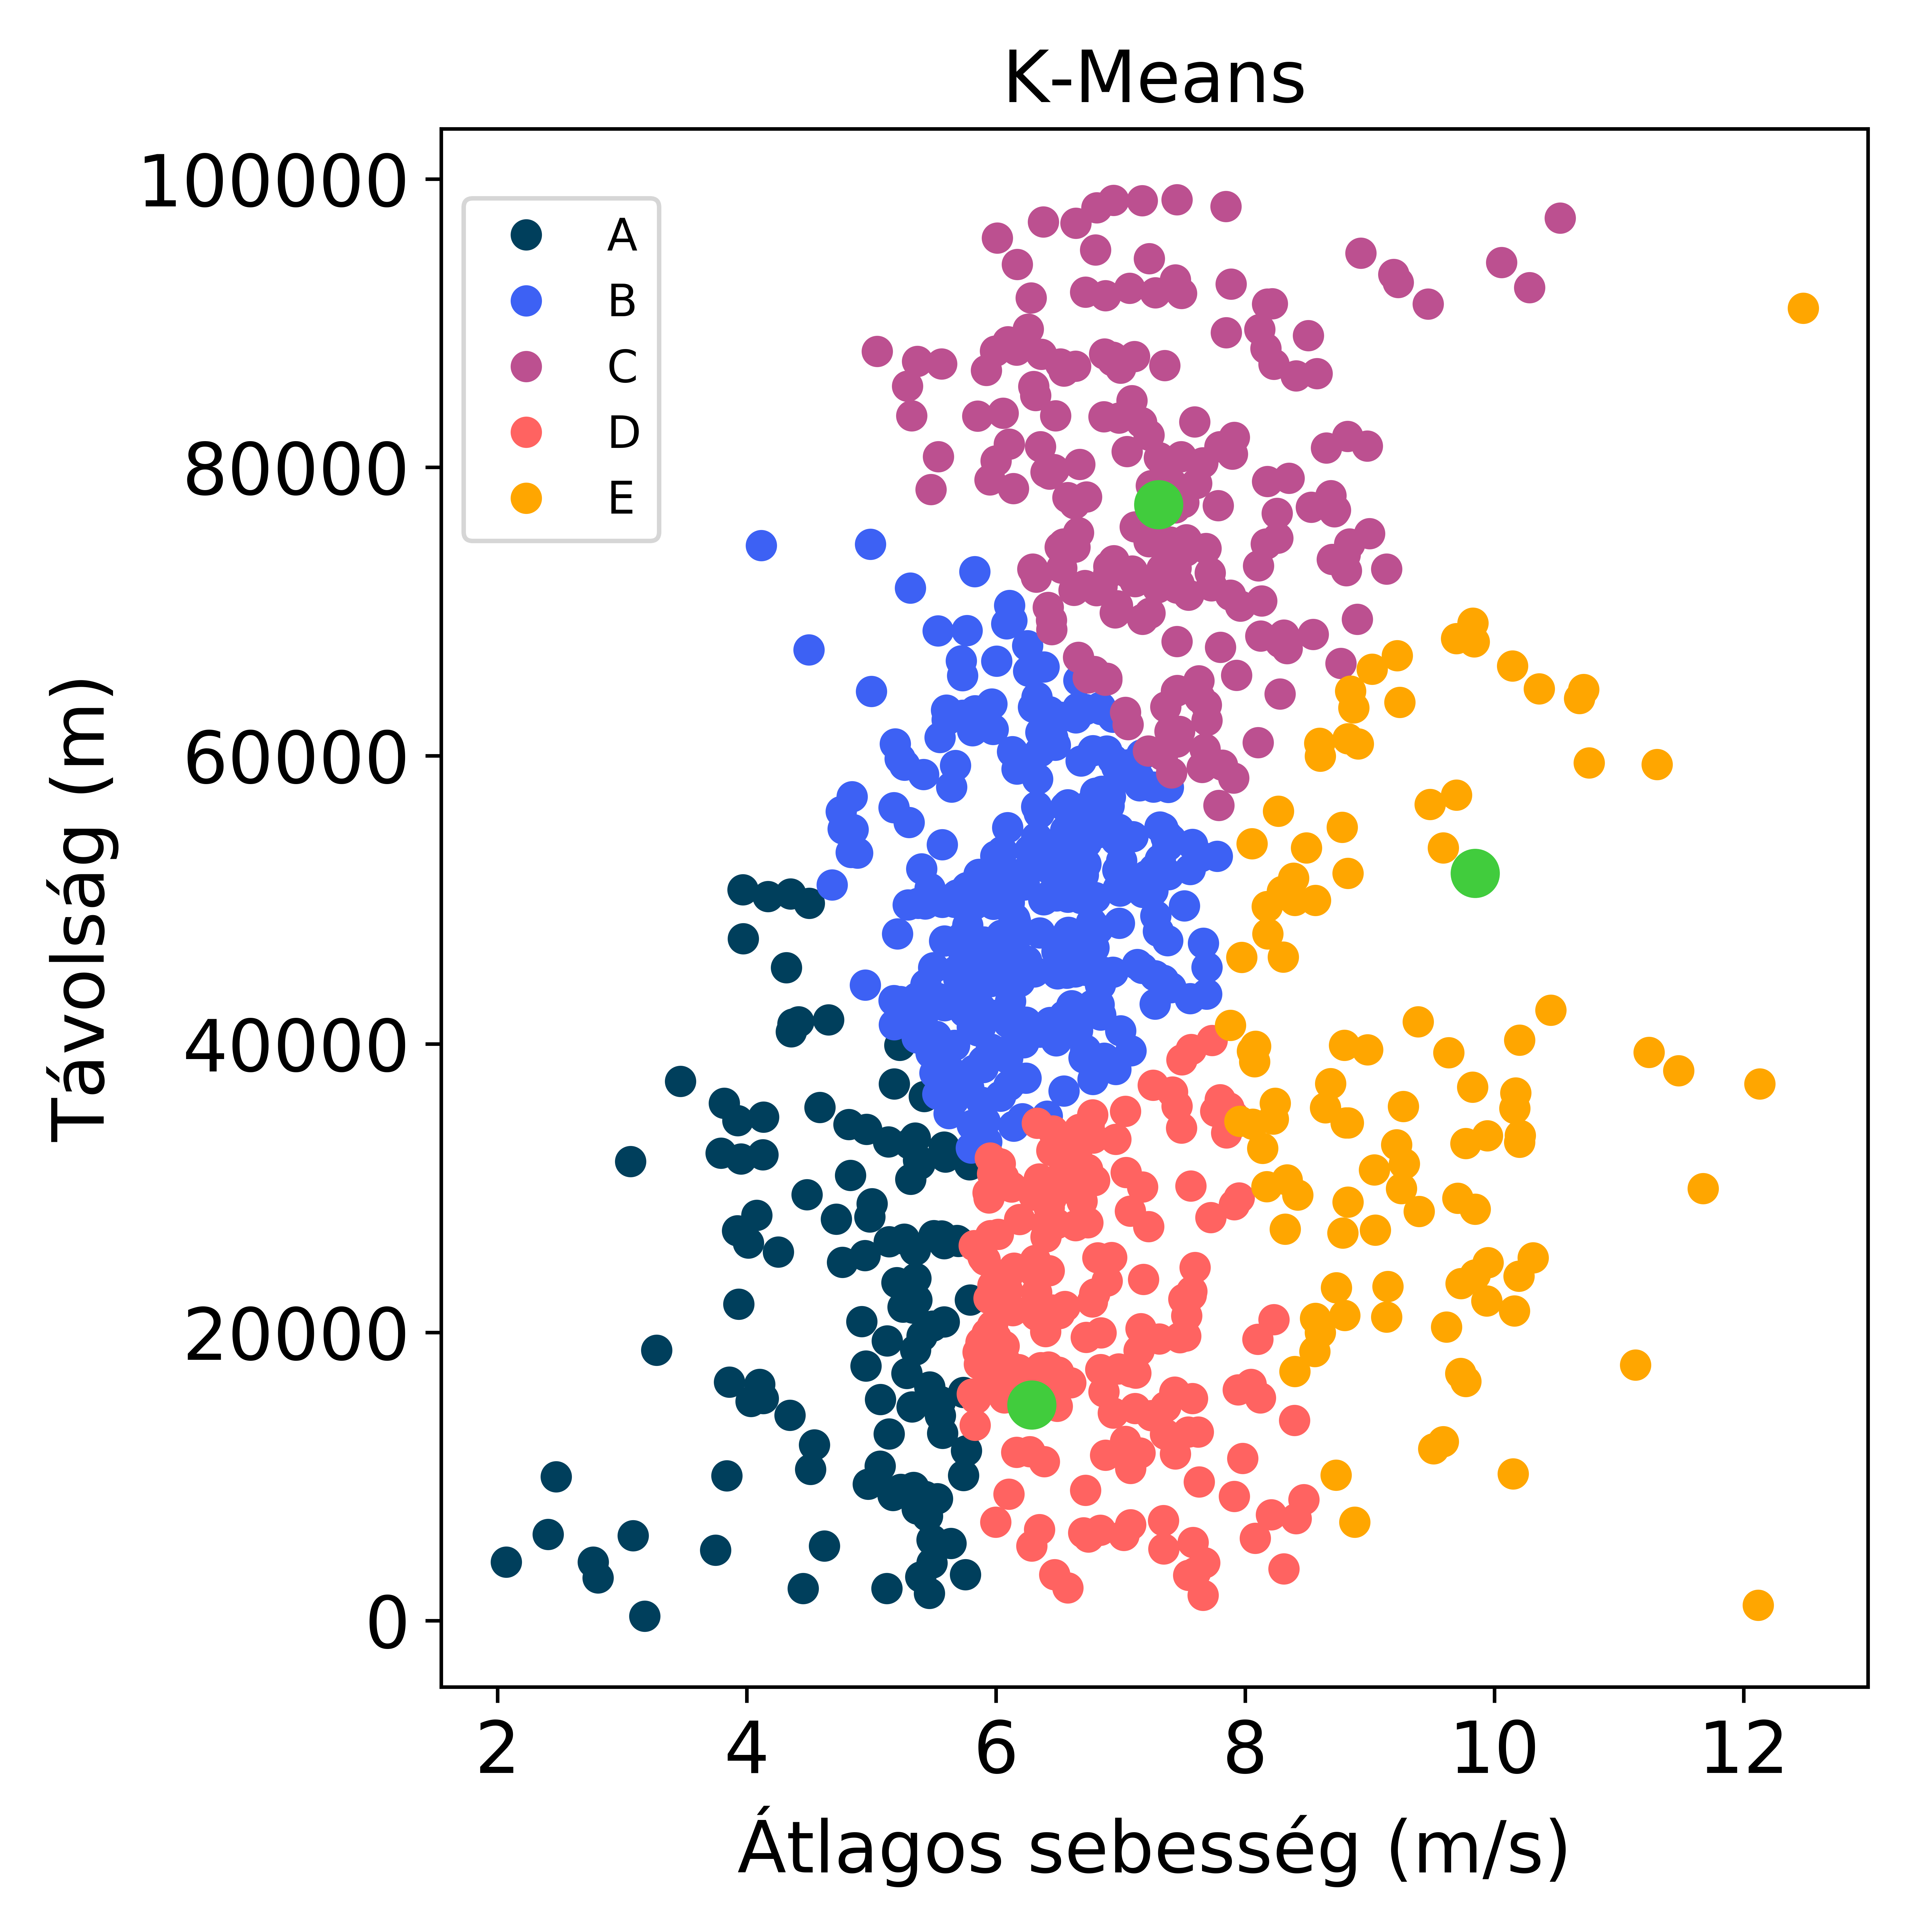
\includegraphics[width=\textwidth,keepaspectratio]{kepek/clustering/age_group_0_training_suggestions.png}
		\caption{ 0. korcsoport}
		\label{subfig:ageNullTraining}
	\end{subfigure}%
	\begin{subfigure}{.5\linewidth}
		\centering
		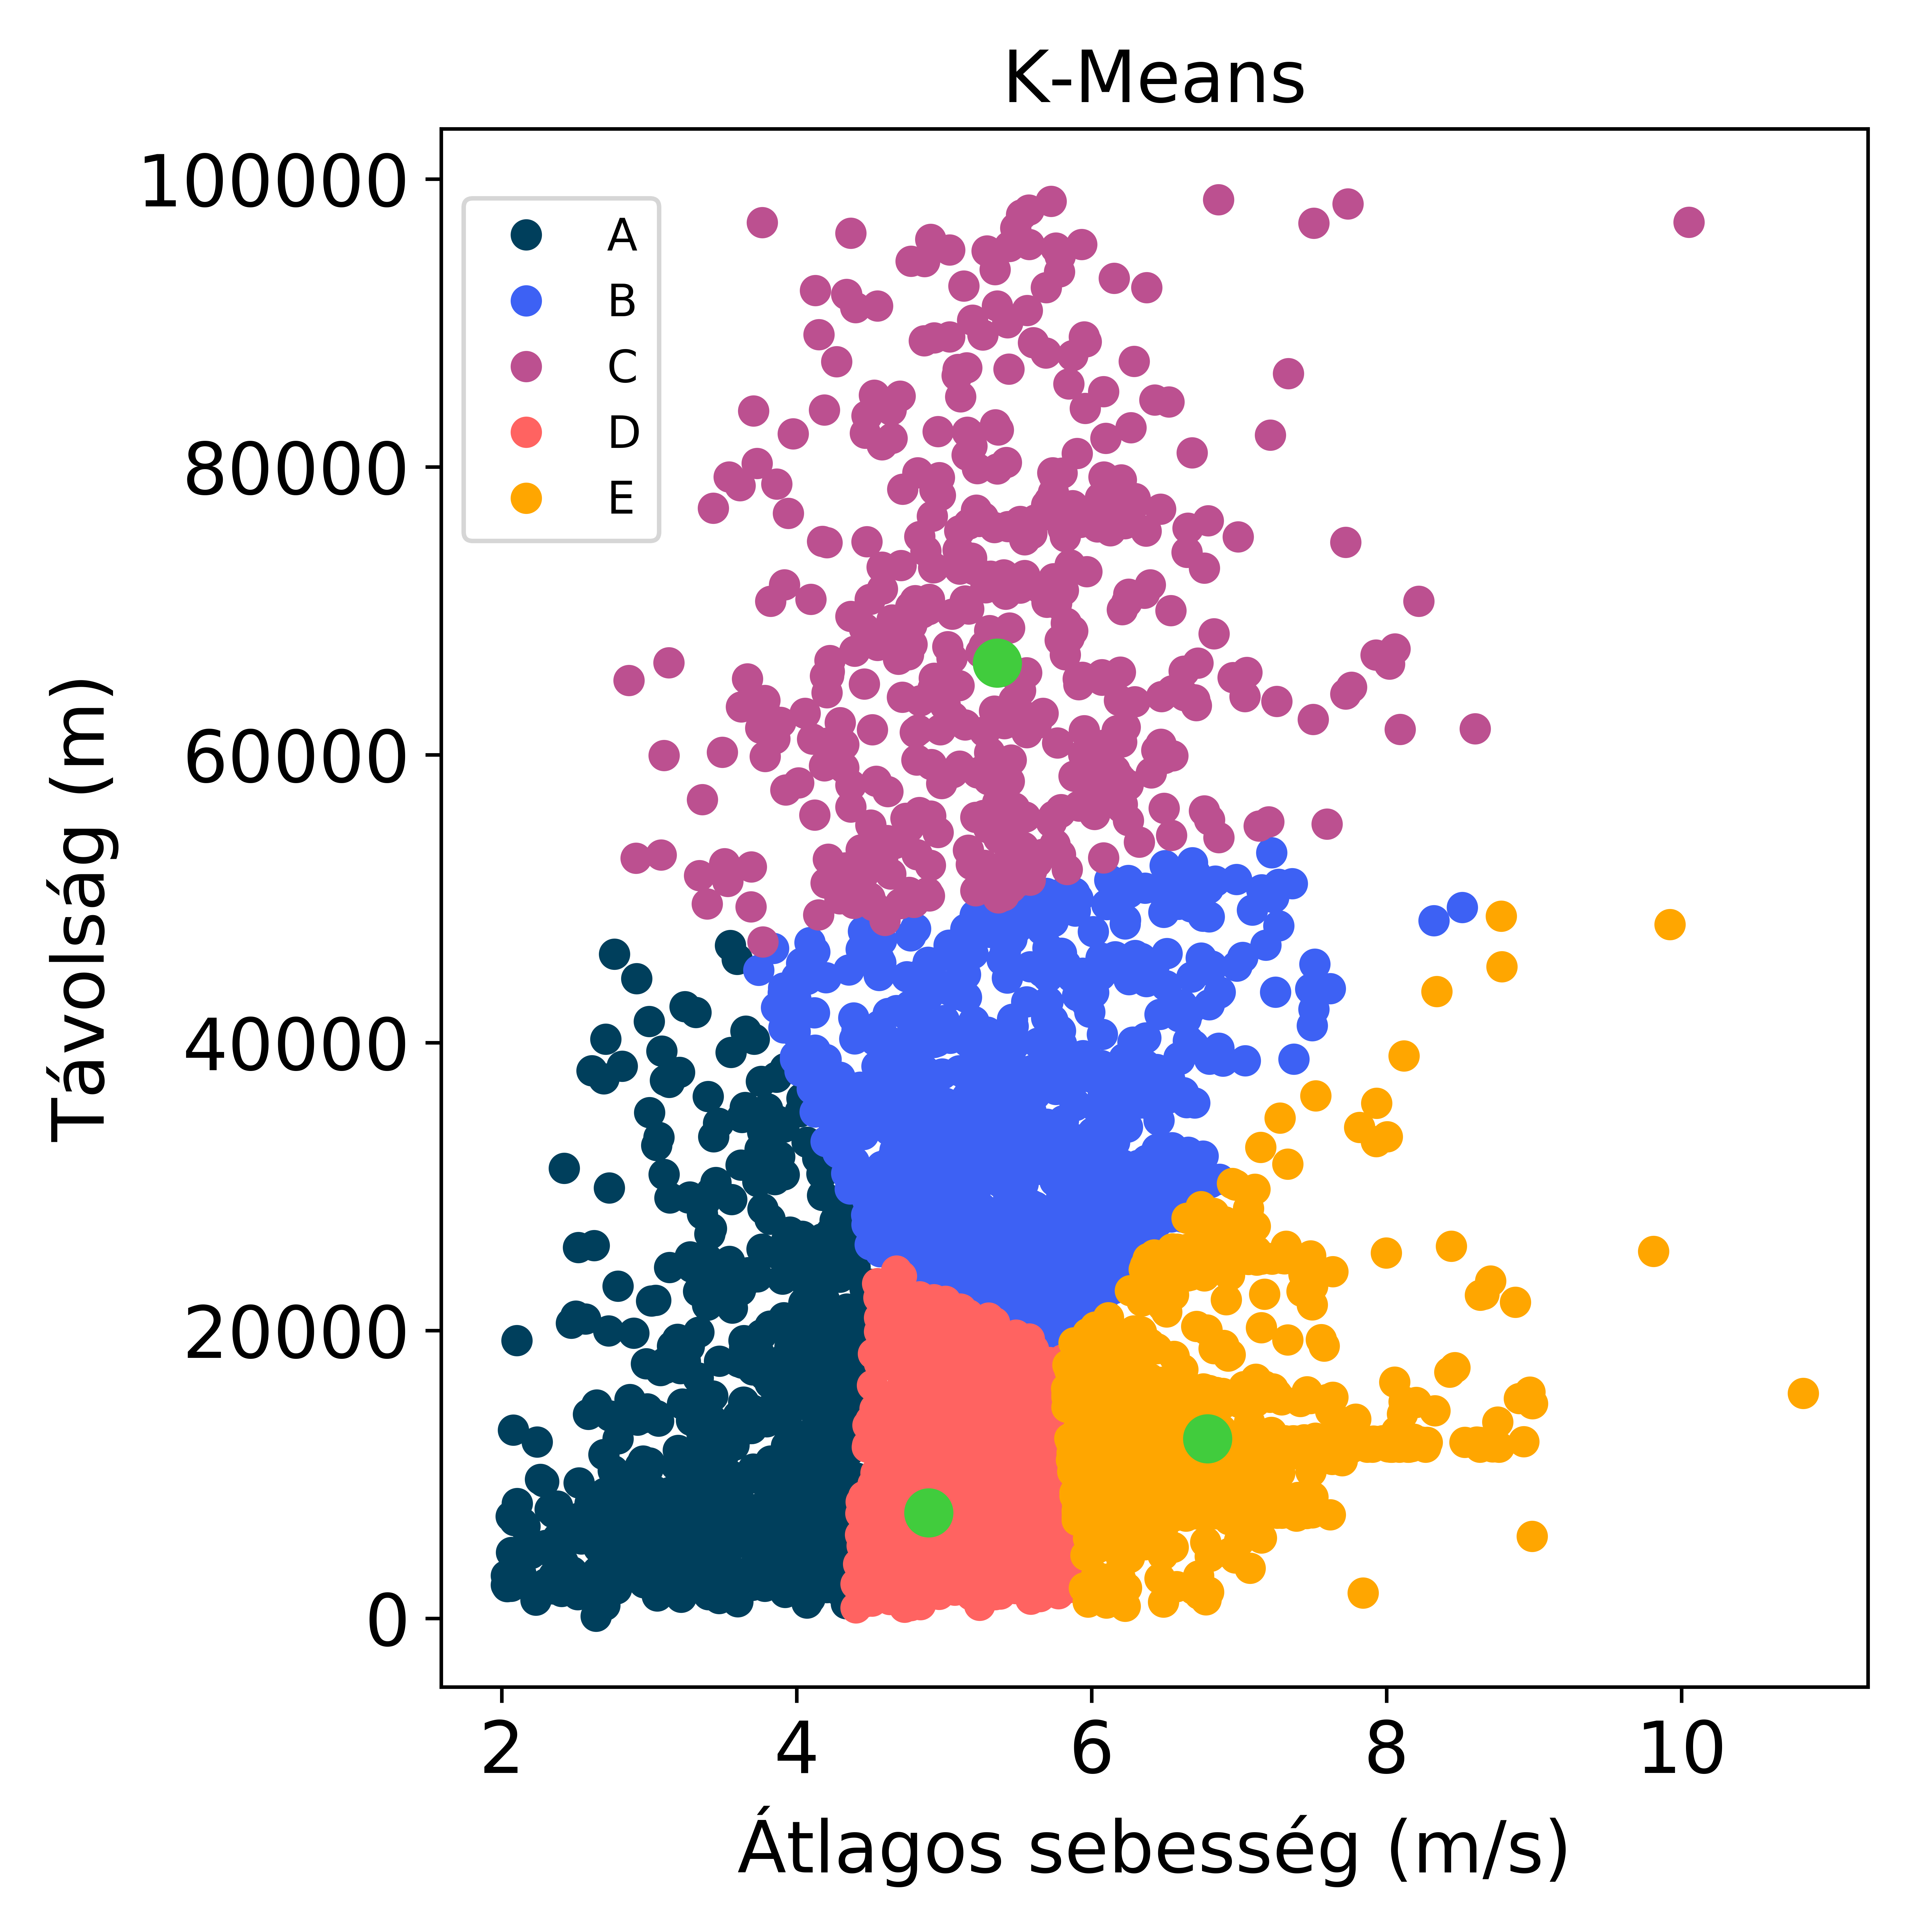
\includegraphics[width=\textwidth,keepaspectratio]{kepek/clustering/age_group_1_training_suggestions.png}
		\caption{1. korcsoport}
		\label{subfig:ageOneTraining}
	\end{subfigure}\\[1ex]
	\begin{subfigure}{.5\linewidth}
		\centering
		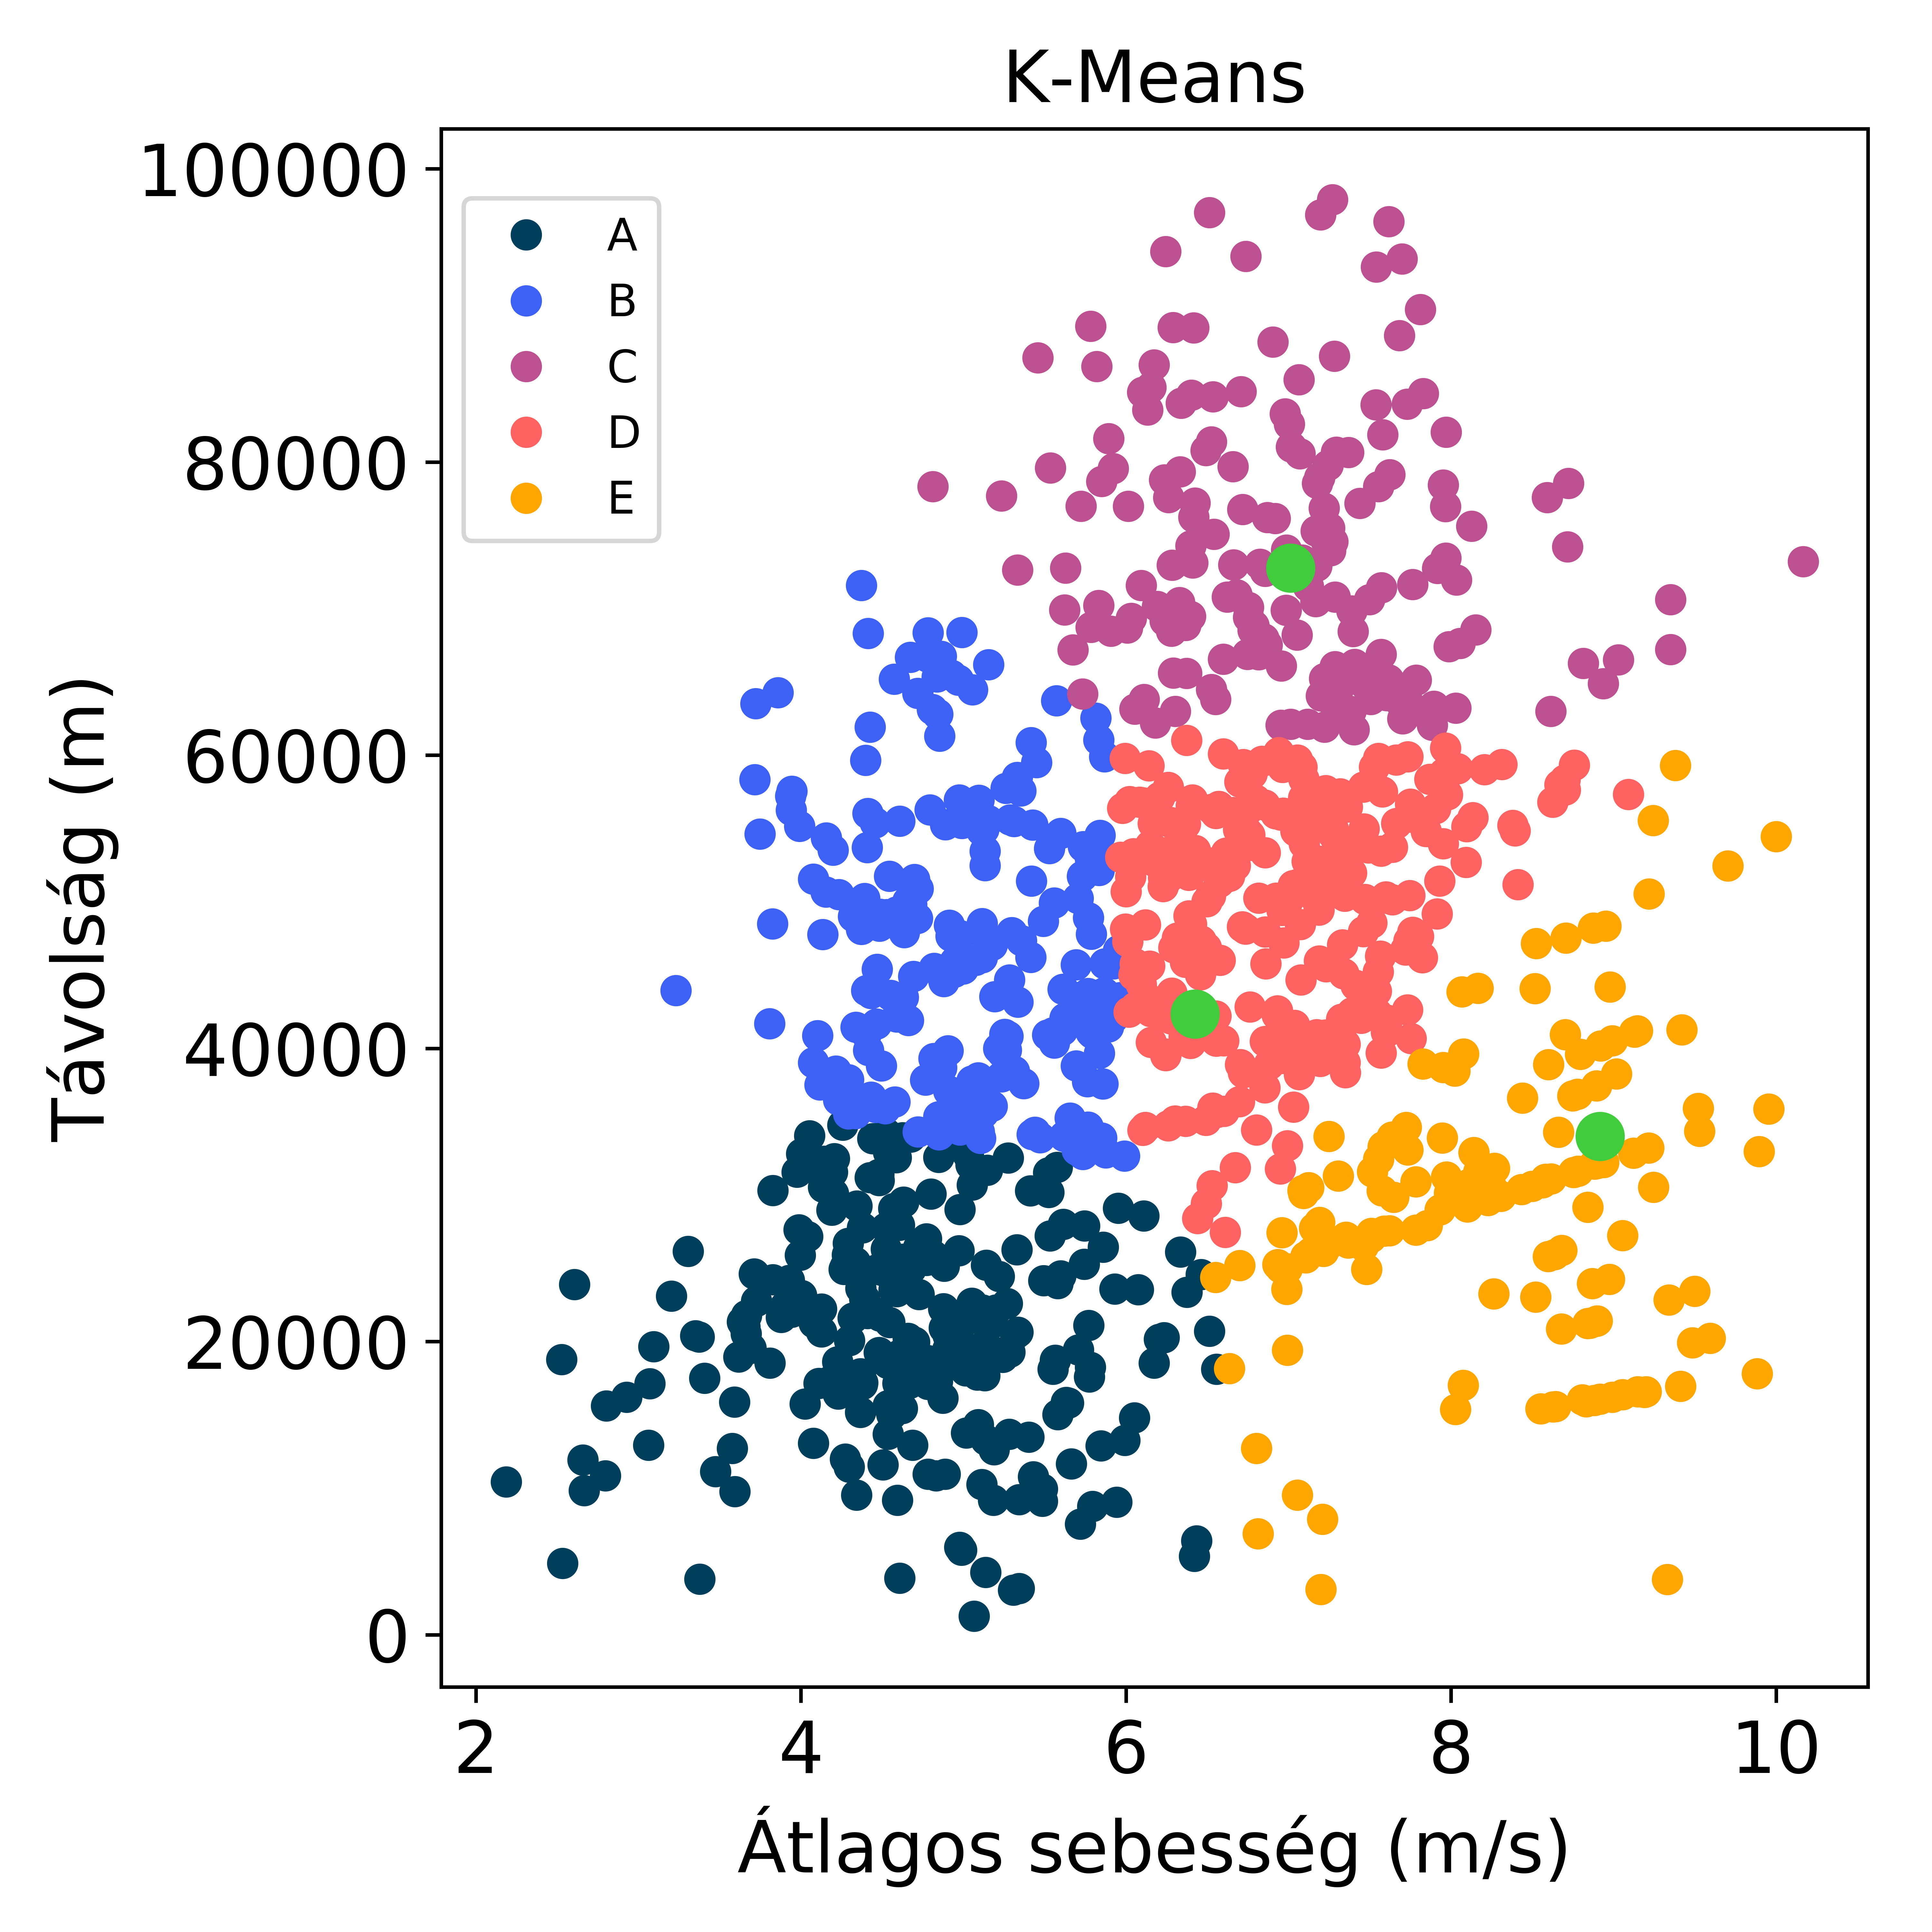
\includegraphics[width=\textwidth,keepaspectratio]{kepek/clustering/age_group_2_training_suggestions.png}
		\caption{2. korcsoport}
		\label{subfig:ageTwoTraining}
	\end{subfigure}
	\caption{Edzés javaslatok a K-Means klaszterezés eredményei alapján}
	\label{fig:traningSuggestions}
\end{figure}

\noindent A 0. korcsoportra készült edzés javaslatok a \myref{subfig:ageNullTraining} ábrán láthatóak. 3 javaslat készült, a C, D és E klaszterek alapján, különböző nehézségi fokozatokkal. 
\begin{itemize}
	\item C klaszter: extrém nagy távolságú, magas és extrém magas átlagsebességű útvonalak, a módszer egy normál fokozatú edzésre tett javaslatot. A javasolt edzés paraméterei:
	\begin{itemize}
		\item távolság: 77410.3 méter (77.4 km)
		\item átlagos sebesség: 7.3 m/s (26.28 km/h)
		\item mozgási idő: 2 óra és 57 perc
	\end{itemize}
	\item D klaszter: normális távolságú, magas átlagsebességű útvonalak, a módszer egy könnyű fokozatú edzésre tett javaslatot. A javasolt edzés paraméterei:
	\begin{itemize}
		\item távolság: 14982.8 méter (14.98 km)
		\item átlagos sebesség: 6.3 m/s (22.68 km/h)
		\item mozgási idő: 40 perc
	\end{itemize}
	\item E klaszter: normális és nagy távolságú, extrém magas átlagsebességű útvonalak, a módszer egy nehéz fokozatú edzésre tett javaslatot. A javasolt edzés paraméterei:
	\begin{itemize}
		\item távolság: 51853.1 méter (51.85 km)
		\item átlagos sebesség: 9.8 m/s (35.28 km/h)
		\item mozgási idő: 1 óra és 28 perc
	\end{itemize}
\end{itemize}

\noindent A 1. korcsoportra készült edzés javaslatok a \myref{subfig:ageOneTraining} ábrán láthatóak. 3 javaslat készült, a C, D és E klaszterek alapján, különböző nehézségi fokozatokkal. 
\begin{itemize}
	\item C klaszter: extrém nagy távolságú, magas és extrém magas átlagsebességű útvonalak, a módszer egy normál fokozatú edzésre tett javaslatot. A javasolt edzés paraméterei:
	\begin{itemize}
		\item távolság: 66389.3 méter (66.39 km)
		\item átlagos sebesség: 5.3 m/s (19.08 km/h)
		\item mozgási idő: 3 óra és 26 perc
	\end{itemize}
	\item D klaszter: normális távolságú, magas átlagsebességű útvonalak, a módszer egy könnyű fokozatú edzésre tett javaslatot. A javasolt edzés paraméterei:
	\begin{itemize}
		\item távolság: 7350.95 méter (7.35 km)
		\item átlagos sebesség: 4.9 m/s (17.64 km/h)
		\item mozgási idő: 25 perc
	\end{itemize}
	\item E klaszter: normális és nagy távolságú, extrém magas átlagsebességű útvonalak, a módszer egy nehéz fokozatú edzésre tett javaslatot. A javasolt edzés paraméterei:
	\begin{itemize}
		\item távolság: 12489.7 méter (12.49 km)
		\item átlagos sebesség: 6.8 m/s (24.48 km/h)
		\item mozgási idő: 31 perc
	\end{itemize}
\end{itemize}



\noindent A 2. korcsoportra készült edzés javaslatok a \myref{subfig:ageTwoTraining} ábrán láthatóak. 3 javaslat készült, a C, D és E klaszterek alapján, különböző nehézségi fokozatokkal. 
\begin{itemize}
	\item C klaszter: extrém nagy távolságú, magas és extrém magas átlagsebességű átlagsebességű útvonalak, a módszer egy normál fokozatú edzésre tett javaslatot. A javasolt edzés paraméterei:
	\begin{itemize}
		\item távolság: 72773.5 méter (72.77 km)
		\item átlagos sebesség: 7.0 m/s (25.2 km/h)
		\item mozgási idő: 2 óra és 53 perc
	\end{itemize}
	\item D klaszter: nagy távolságú, magas átlagsebességű útvonalak, a módszer könnyű fokozatú edzésre tett javaslatot. A javasolt edzés paraméterei:
	\begin{itemize}
		\item távolság: 42353.25 méter (42.35 km)
		\item átlagos sebesség: 6.4 m/s (23.0 km/h)
		\item mozgási idő: 1 óra és 50 perc
	\end{itemize}
	\item E klaszter: normális távolság, extrém magas átlagsebességű útvonalak, a módszer egy nehéz fokozatú edzésre tett javaslatot. A javasolt edzés paraméterei:
	\begin{itemize}
		\item távolság: 33997.5 méter (34.0 km)
		\item átlagos sebesség: 8.9 m/s (32.04 km/h)
		\item mozgási idő: 1 óra és 4 perc
	\end{itemize}
\end{itemize}



A kapott edzés javaslatok között jól látható különbség van, az egyes korcsoportokra jellemző útvonalakhoz igazodva egyedi eredményeket adnak. Az edzés tervezés már ezzel az alapvető módszerrel megvalósítva is a felhasználó kora alapján skálázódik, ezzel korcsoportokra szabott, specifikus javaslat tételt téve lehetővé.














% =======================================================

